%%%%%%%%%%%%%%%%%%%%%%%%%%%%%%%%%%%%%%%%%
%  My documentation report
%  Objetive: Explain what I did and how, so someone can continue with the investigation
%
% Important note:
% Chapter heading images should have a 2:1 width:height ratio,
% e.g. 920px width and 460px height.
%
%%%%%%%%%%%%%%%%%%%%%%%%%%%%%%%%%%%%%%%%%


%----------------------------------------------------------------------------------------
%	PACKAGES AND OTHER DOCUMENT CONFIGURATIONS
%----------------------------------------------------------------------------------------

\documentclass[11pt,fleqn]{book} % Default font size and left-justified equations

\usepackage[top=3cm,bottom=3cm,left=3.2cm,right=3.2cm,headsep=10pt,letterpaper]{geometry} % Page margins
\usepackage{tikz-cd}
\usetikzlibrary{arrows.meta,shapes.geometric,shapes.misc,positioning,calc}
\usepackage{xcolor} % Required for specifying colors by name
\definecolor{ocre}{RGB}{52,177,201} % Define the orange color used for highlighting throughout the book

% Font Settings
\usepackage{avant} % Use the Avantgarde font for headings
%\usepackage{times} % Use the Times font for headings
\usepackage{microtype} % Slightly tweak font spacing for aesthetics
\usepackage[utf8]{inputenc} % Required for including letters with accents
\usepackage[T1]{fontenc} % Use 8-bit encoding that has 256 glyphs
\usepackage{amsthm}
\usepackage[most]{tcolorbox}
\usepackage{vwcol}  
\usepackage{multicol}
% Define a new command for the idea callout box
\newtcolorbox{ideabox}[1][]{colback=blue!10!white, colframe=blue!75!black, title=Idea, fonttitle=\bfseries, #1}
% Big Idea callout box
\newtcolorbox{bigidea}[1][]{
  enhanced,
  breakable,
  colback=yellow!10!white,         % background
  colbacktitle=yellow!40!white,   % title background
  colframe=orange!80!black,       % border color
  coltitle=black,                 % title text color
  fonttitle=\bfseries\Large,      % title font
  boxrule=1pt,                    % border thickness
  arc=6pt,                        % rounded corners
  outer arc=2pt,
  left=6pt, right=6pt, top=8pt, bottom=8pt,
  drop shadow=black!50!white,     % shadow
  title=Big Idea,               % default title with icon
  #1
}
\newtcolorbox{conceptbox}[1][]{
  enhanced,
  breakable,
  colback=purple!8!white,        % soft background
  colbacktitle=purple!20!white,  % title background
  colframe=purple!70!black,      % border color
  coltitle=black,                % title text color
  fonttitle=\bfseries\large,     % title font
  boxrule=1pt,                   % border thickness
  arc=6pt,                       % rounded corners
  outer arc=2pt,
  left=6pt, right=6pt, top=8pt, bottom=8pt,
  drop shadow=black!40!white,    % subtle shadow
  title=Where in the Universe?,  % default title
  #1
}

% Bibliography
% Bibliography
\usepackage[numbers,sort&compress]{natbib}


%----------------------------------------------------------------------------------------
%	VARIOUS REQUIRED PACKAGES
%----------------------------------------------------------------------------------------

\usepackage{titlesec} % Allows customization of titles

\usepackage{graphicx} % Required for including pictures
\graphicspath{{Pictures/}} % Specifies the directory where pictures are stored
% \graphicspath{{Plots/}}
\usepackage{lipsum} % Inserts dummy text

\usepackage{tikz} % Required for drawing custom shapes

\usepackage[english]{babel} % English language/hyphenation

\usepackage{enumitem} % Customize lists
\setlist{nolistsep} % Reduce spacing between bullet points and numbered lists

\usepackage{booktabs} % Required for nicer horizontal rules in tables

\usepackage{eso-pic} % Required for specifying an image background in the title page

%----------------------------------------------------------------------------------------
%	MAIN TABLE OF CONTENTS
%----------------------------------------------------------------------------------------

\usepackage{titletoc} % Required for manipulating the table of contents

\contentsmargin{0cm} % Removes the default margin
% Chapter text styling
\titlecontents{chapter}[1.25cm] % Indentation
{\addvspace{15pt}\large\sffamily\bfseries} % Spacing and font options for chapters
{\color{ocre!60}\contentslabel[\Large\thecontentslabel]{1.25cm}\color{ocre}} % Chapter number
{}  
{\color{ocre!60}\normalsize\sffamily\bfseries\;\titlerule*[.5pc]{.}\;\thecontentspage} % Page number
% Section text styling
\titlecontents{section}[1.25cm] % Indentation
{\addvspace{5pt}\sffamily\bfseries} % Spacing and font options for sections
{\contentslabel[\thecontentslabel]{1.25cm}} % Section number
{}
{\sffamily\hfill\color{black}\thecontentspage} % Page number
[]
% Subsection text styling
\titlecontents{subsection}[1.25cm] % Indentation
{\addvspace{1pt}\sffamily\small} % Spacing and font options for subsections
{\contentslabel[\thecontentslabel]{1.25cm}} % Subsection number
{}
{\sffamily\;\titlerule*[.5pc]{.}\;\thecontentspage} % Page number
[] 

%----------------------------------------------------------------------------------------
%	MINI TABLE OF CONTENTS IN CHAPTER HEADS
%----------------------------------------------------------------------------------------

% Section text styling
\titlecontents{lsection}[0em] % Indendating
{\footnotesize\sffamily} % Font settings
{}
{}
{}

% Subsection text styling
\titlecontents{lsubsection}[.5em] % Indentation
{\normalfont\footnotesize\sffamily} % Font settings
{}
{}
{}
 
%----------------------------------------------------------------------------------------
%	PAGE HEADERS
%----------------------------------------------------------------------------------------

\usepackage{fancyhdr} % Required for header and footer configuration

\pagestyle{fancy}
\renewcommand{\chaptermark}[1]{\markboth{\sffamily\normalsize\bfseries\chaptername\ \thechapter.\ #1}{}} % Chapter text font settings
\renewcommand{\sectionmark}[1]{\markright{\sffamily\normalsize\thesection\hspace{5pt}#1}{}} % Section text font settings
\fancyhf{} \fancyhead[LE,RO]{\sffamily\normalsize\thepage} % Font setting for the page number in the header
\fancyhead[LO]{\rightmark} % Print the nearest section name on the left side of odd pages
\fancyhead[RE]{\leftmark} % Print the current chapter name on the right side of even pages
\renewcommand{\headrulewidth}{0.5pt} % Width of the rule under the header
\addtolength{\headheight}{2.5pt} % Increase the spacing around the header slightly
\renewcommand{\footrulewidth}{0pt} % Removes the rule in the footer
\fancypagestyle{plain}{\fancyhead{}\renewcommand{\headrulewidth}{0pt}} % Style for when a plain pagestyle is specified

% Removes the header from odd empty pages at the end of chapters
\makeatletter
\renewcommand{\cleardoublepage}{
\clearpage\ifodd\c@page\else
\hbox{}
\vspace*{\fill}
\thispagestyle{empty}
\newpage
\fi}

%----------------------------------------------------------------------------------------
%	THEOREM STYLES
%----------------------------------------------------------------------------------------

\usepackage{amsmath,amsfonts,amssymb,amsthm} % For math equations, theorems, symbols, etc

\newcommand{\intoo}[2]{\mathopen{]}#1\,;#2\mathclose{[}}
\newcommand{\ud}{\mathop{\mathrm{{}d}}\mathopen{}}
\newcommand{\intff}[2]{\mathopen{[}#1\,;#2\mathclose{]}}
\newtheorem{notation}{Notation}[chapter]

%%%%%%%%%%%%%%%%%%%%%%%%%%%%%%%%%%%%%%%%%%%%%%%%%%%%%%%%%%%%%%%%%%%%%%%%%%%
%%%%%%%%%%%%%%%%%%%% dedicated to boxed/framed environements %%%%%%%%%%%%%%
%%%%%%%%%%%%%%%%%%%%%%%%%%%%%%%%%%%%%%%%%%%%%%%%%%%%%%%%%%%%%%%%%%%%%%%%%%%
\newtheoremstyle{ocrenumbox}% % Theorem style name
{0pt}% Space above
{0pt}% Space below
{\normalfont}% % Body font
{}% Indent amount
{\small\bf\sffamily\color{ocre}}% % Theorem head font
{\;}% Punctuation after theorem head
{0.25em}% Space after theorem head
{\small\sffamily\color{ocre}\thmname{#1}\nobreakspace\thmnumber{\@ifnotempty{#1}{}\@upn{#2}}% Theorem text (e.g. Theorem 2.1)
\thmnote{\nobreakspace\the\thm@notefont\sffamily\bfseries\color{black}---\nobreakspace#3.}} % Optional theorem note
\renewcommand{\qedsymbol}{$\blacksquare$}% Optional qed square

\newtheoremstyle{blacknumex}% Theorem style name
{5pt}% Space above
{5pt}% Space below
{\normalfont}% Body font
{} % Indent amount
{\small\bf\sffamily}% Theorem head font
{\;}% Punctuation after theorem head
{0.25em}% Space after theorem head
{\small\sffamily{\tiny\ensuremath{\blacksquare}}\nobreakspace\thmname{#1}\nobreakspace\thmnumber{\@ifnotempty{#1}{}\@upn{#2}}% Theorem text (e.g. Theorem 2.1)
\thmnote{\nobreakspace\the\thm@notefont\sffamily\bfseries---\nobreakspace#3.}}% Optional theorem note

\newtheoremstyle{blacknumbox} % Theorem style name
{0pt}% Space above
{0pt}% Space below
{\normalfont}% Body font
{}% Indent amount
{\small\bf\sffamily}% Theorem head font
{\;}% Punctuation after theorem head
{0.25em}% Space after theorem head
{\small\sffamily\thmname{#1}\nobreakspace\thmnumber{\@ifnotempty{#1}{}\@upn{#2}}% Theorem text (e.g. Theorem 2.1)
\thmnote{\nobreakspace\the\thm@notefont\sffamily\bfseries---\nobreakspace#3.}}% Optional theorem note

%%%%%%%%%%%%%%%%%%%%%%%%%%%%%%%%%%%%%%%%%%%%%%%%%%%%%%%%%%%%%%%%%%%%%%%%%%%
%%%%%%%%%%%%% dedicated to non-boxed/non-framed environements %%%%%%%%%%%%%
%%%%%%%%%%%%%%%%%%%%%%%%%%%%%%%%%%%%%%%%%%%%%%%%%%%%%%%%%%%%%%%%%%%%%%%%%%%
\newtheoremstyle{ocrenum}% % Theorem style name
{5pt}% Space above
{5pt}% Space below
{\normalfont}% % Body font
{}% Indent amount
{\small\bf\sffamily\color{ocre}}% % Theorem head font
{\;}% Punctuation after theorem head
{0.25em}% Space after theorem head
{\small\sffamily\color{ocre}\thmname{#1}\nobreakspace\thmnumber{\@ifnotempty{#1}{}\@upn{#2}}% Theorem text (e.g. Theorem 2.1)
\thmnote{\nobreakspace\the\thm@notefont\sffamily\bfseries\color{black}---\nobreakspace#3.}} % Optional theorem note
\renewcommand{\qedsymbol}{$\blacksquare$}% Optional qed square
\makeatother

% Defines the theorem text style for each type of theorem to one of the three styles above
\newcounter{dummy} 
\numberwithin{dummy}{section}
\theoremstyle{ocrenumbox}


\newtheorem{theoremeT}[dummy]{Theorem}
\newtheorem{lemma}[dummy]{Lemma}
\newtheorem{observation}[dummy]{Observation}
\newtheorem{proposition}[dummy]{Proposition}
% \newtheorem{definition}[dummy]{Definition}
\newtheorem{claim}[dummy]{Claim}
\newtheorem{fact}[dummy]{Fact}
\newtheorem{assumption}[dummy]{Assumption}

\newtheorem{problem}{Problem}[chapter]
% \newtheorem{exercise}{Exercise}[chapter]
\theoremstyle{blacknumex}
\newtheorem{exampleT}{Example}[chapter]
\theoremstyle{blacknumbox}
\newtheorem{vocabulary}{Vocabulary}[chapter]
\newtheorem{definitionT}{Definition}[section]
\newtheorem{corollaryT}[dummy]{Corollary}
\theoremstyle{ocrenum}

%----------------------------------------------------------------------------------------
%	DEFINITION OF COLORED BOXES
%----------------------------------------------------------------------------------------

\RequirePackage[framemethod=default]{mdframed} % Required for creating the theorem, definition, exercise and corollary boxes

% Theorem box
\newmdenv[skipabove=7pt,
skipbelow=7pt,
backgroundcolor=black!5,
linecolor=ocre,
innerleftmargin=5pt,
innerrightmargin=5pt,
innertopmargin=5pt,
leftmargin=0cm,
rightmargin=0cm,
innerbottommargin=5pt]{tBox}

% Exercise box	  
\newmdenv[skipabove=7pt,
skipbelow=7pt,
rightline=false,
leftline=true,
topline=false,
bottomline=false,
backgroundcolor=ocre!10,
linecolor=ocre,
innerleftmargin=5pt,
innerrightmargin=5pt,
innertopmargin=5pt,
innerbottommargin=5pt,
leftmargin=0cm,
rightmargin=0cm,
linewidth=4pt]{eBox}	

% Definition box
\newmdenv[skipabove=7pt,
skipbelow=7pt,
rightline=false,
leftline=true,
topline=false,
bottomline=false,
linecolor=ocre,
innerleftmargin=5pt,
innerrightmargin=5pt,
innertopmargin=0pt,
leftmargin=0cm,
rightmargin=0cm,
linewidth=4pt,
innerbottommargin=0pt]{dBox}	

% Corollary box
\newmdenv[skipabove=7pt,
skipbelow=7pt,
rightline=false,
leftline=true,
topline=false,
bottomline=false,
linecolor=gray,
backgroundcolor=black!5,
innerleftmargin=5pt,
innerrightmargin=5pt,
innertopmargin=5pt,
leftmargin=0cm,
rightmargin=0cm,
linewidth=4pt,
innerbottommargin=5pt]{cBox}

% Creates an environment for each type of theorem and assigns it a theorem text style from the "Theorem Styles" section above and a colored box from above
\newenvironment{theorem}{\begin{tBox}\begin{theoremeT}}{\end{theoremeT}\end{tBox}}
\newenvironment{exercise}{\begin{eBox}\begin{exerciseT}}{\hfill{\color{ocre}\tiny\ensuremath{\blacksquare}}\end{exerciseT}\end{eBox}}				  
\newenvironment{definition}{\begin{dBox}\begin{definitionT}}{\end{definitionT}\end{dBox}}	
\newenvironment{example}{\begin{exampleT}}{\hfill{\tiny\ensuremath{\blacksquare}}\end{exampleT}}		
\newenvironment{corollary}{\begin{cBox}\begin{corollaryT}}{\end{corollaryT}\end{cBox}}	

%----------------------------------------------------------------------------------------
%	REMARK ENVIRONMENT
%----------------------------------------------------------------------------------------

\newenvironment{remark}{\par\vspace{10pt}\small % Vertical white space above the remark and smaller font size
\begin{list}{}{
\leftmargin=35pt % Indentation on the left
\rightmargin=25pt}\item\ignorespaces % Indentation on the right
\makebox[-2.5pt]{\begin{tikzpicture}[overlay]
\node[draw=ocre!60,line width=1pt,circle,fill=ocre!25,font=\sffamily\bfseries,inner sep=2pt,outer sep=0pt] at (-15pt,0pt){\textcolor{ocre}{R}};\end{tikzpicture}} % Orange R in a circle
\advance\baselineskip -1pt}{\end{list}\vskip5pt} % Tighter line spacing and white space after remark

%----------------------------------------------------------------------------------------
%	SECTION NUMBERING IN THE MARGIN
%----------------------------------------------------------------------------------------

\makeatletter
\renewcommand{\@seccntformat}[1]{\llap{\textcolor{ocre}{\csname the#1\endcsname}\hspace{1em}}}                    
\renewcommand{\section}{\@startsection{section}{1}{\z@}
{-4ex \@plus -1ex \@minus -.4ex}
{1ex \@plus.2ex }
{\normalfont\large\sffamily\bfseries}}
\renewcommand{\subsection}{\@startsection {subsection}{2}{\z@}
{-3ex \@plus -0.1ex \@minus -.4ex}
{0.5ex \@plus.2ex }
{\normalfont\sffamily\bfseries}}
\renewcommand{\subsubsection}{\@startsection {subsubsection}{3}{\z@}
{-2ex \@plus -0.1ex \@minus -.2ex}
{.2ex \@plus.2ex }
{\normalfont\small\sffamily\bfseries}}                        
\renewcommand\paragraph{\@startsection{paragraph}{4}{\z@}
{-2ex \@plus-.2ex \@minus .2ex}
{.1ex}
{\normalfont\small\sffamily\bfseries}}

%----------------------------------------------------------------------------------------
%	HYPERLINKS IN THE DOCUMENTS
%----------------------------------------------------------------------------------------

% For an unclear reason, the package should be loaded now and not later
\usepackage{hyperref}
\hypersetup{hidelinks,backref=true,pagebackref=true,hyperindex=true,colorlinks=false,breaklinks=true,urlcolor= ocre,bookmarks=true,bookmarksopen=false,pdftitle={Title},pdfauthor={Author}}

%----------------------------------------------------------------------------------------
%	CHAPTER HEADINGS
%----------------------------------------------------------------------------------------

% The set-up below should be (sadly) manually adapted to the overall margin page septup controlled by the geometry package loaded in the main.tex document. It is possible to implement below the dimensions used in the goemetry package (top,bottom,left,right)... TO BE DONE

\newcommand{\thechapterimage}{}
\newcommand{\chapterimage}[1]{\renewcommand{\thechapterimage}{#1}}

% Numbered chapters with mini tableofcontents
\def\thechapter{\arabic{chapter}}
\def\@makechapterhead#1{
\thispagestyle{empty}
{\centering \normalfont\sffamily
\ifnum \c@secnumdepth >\m@ne
\if@mainmatter
\startcontents
\begin{tikzpicture}[remember picture,overlay]
\node at (current page.north west)
{\begin{tikzpicture}[remember picture,overlay]
\node[anchor=north west,inner sep=0pt] at (0,0) {\includegraphics[width=\paperwidth]{\thechapterimage}};
%%%%%%%%%%%%%%%%%%%%%%%%%%%%%%%%%%%%%%%%%%%%%%%%%%%%%%%%%%%%%%%%%%%%%%%%%%%%%%%%%%%%%
% Commenting the 3 lines below removes the small contents box in the chapter heading
%\fill[color=ocre!10!white,opacity=.6] (1cm,0) rectangle (8cm,-7cm);
%\node[anchor=north west] at (1.1cm,.35cm) {\parbox[t][8cm][t]{6.5cm}{\huge\bfseries\flushleft \printcontents{l}{1}{\setcounter{tocdepth}{2}}}};
\draw[anchor=west] (5cm,-9cm) node [rounded corners=20pt,fill=ocre!10!white,text opacity=1,draw=ocre,draw opacity=1,line width=1.5pt,fill opacity=.6,inner sep=12pt]{\huge\sffamily\bfseries\textcolor{black}{\thechapter. #1\strut\makebox[22cm]{}}};
%%%%%%%%%%%%%%%%%%%%%%%%%%%%%%%%%%%%%%%%%%%%%%%%%%%%%%%%%%%%%%%%%%%%%%%%%%%%%%%%%%%%%
\end{tikzpicture}};
\end{tikzpicture}}
\par\vspace*{230\p@}
\fi
\fi}

% Unnumbered chapters without mini tableofcontents (could be added though) 
\def\@makeschapterhead#1{
\thispagestyle{empty}
{\centering \normalfont\sffamily
\ifnum \c@secnumdepth >\m@ne
\if@mainmatter
\begin{tikzpicture}[remember picture,overlay]
\node at (current page.north west)
{\begin{tikzpicture}[remember picture,overlay]
\node[anchor=north west,inner sep=0pt] at (0,0) {\includegraphics[width=\paperwidth]{\thechapterimage}};
\draw[anchor=west] (5cm,-9cm) node [rounded corners=20pt,fill=ocre!10!white,fill opacity=.6,inner sep=12pt,text opacity=1,draw=ocre,draw opacity=1,line width=1.5pt]{\huge\sffamily\bfseries\textcolor{black}{#1\strut\makebox[22cm]{}}};
\end{tikzpicture}};
\end{tikzpicture}}
\par\vspace*{230\p@}
\fi
\fi
}
\makeatother

\NewDocumentCommand{\rmk}{+m}{
    {\it \color{blue!50!white}#1}
}
 % Insert the commands.tex file which contains the majority of the structure behind the template

%----------------------------------------------------------------------------------------
%	Definitions of new commands
%----------------------------------------------------------------------------------------

\def\R{\mathbb{R}}
\newcommand{\cvx}{convex}
\begin{document}

%----------------------------------------------------------------------------------------
%	TITLE PAGE
%----------------------------------------------------------------------------------------

\begingroup
\thispagestyle{empty}
\AddToShipoutPicture*{\put(0,0){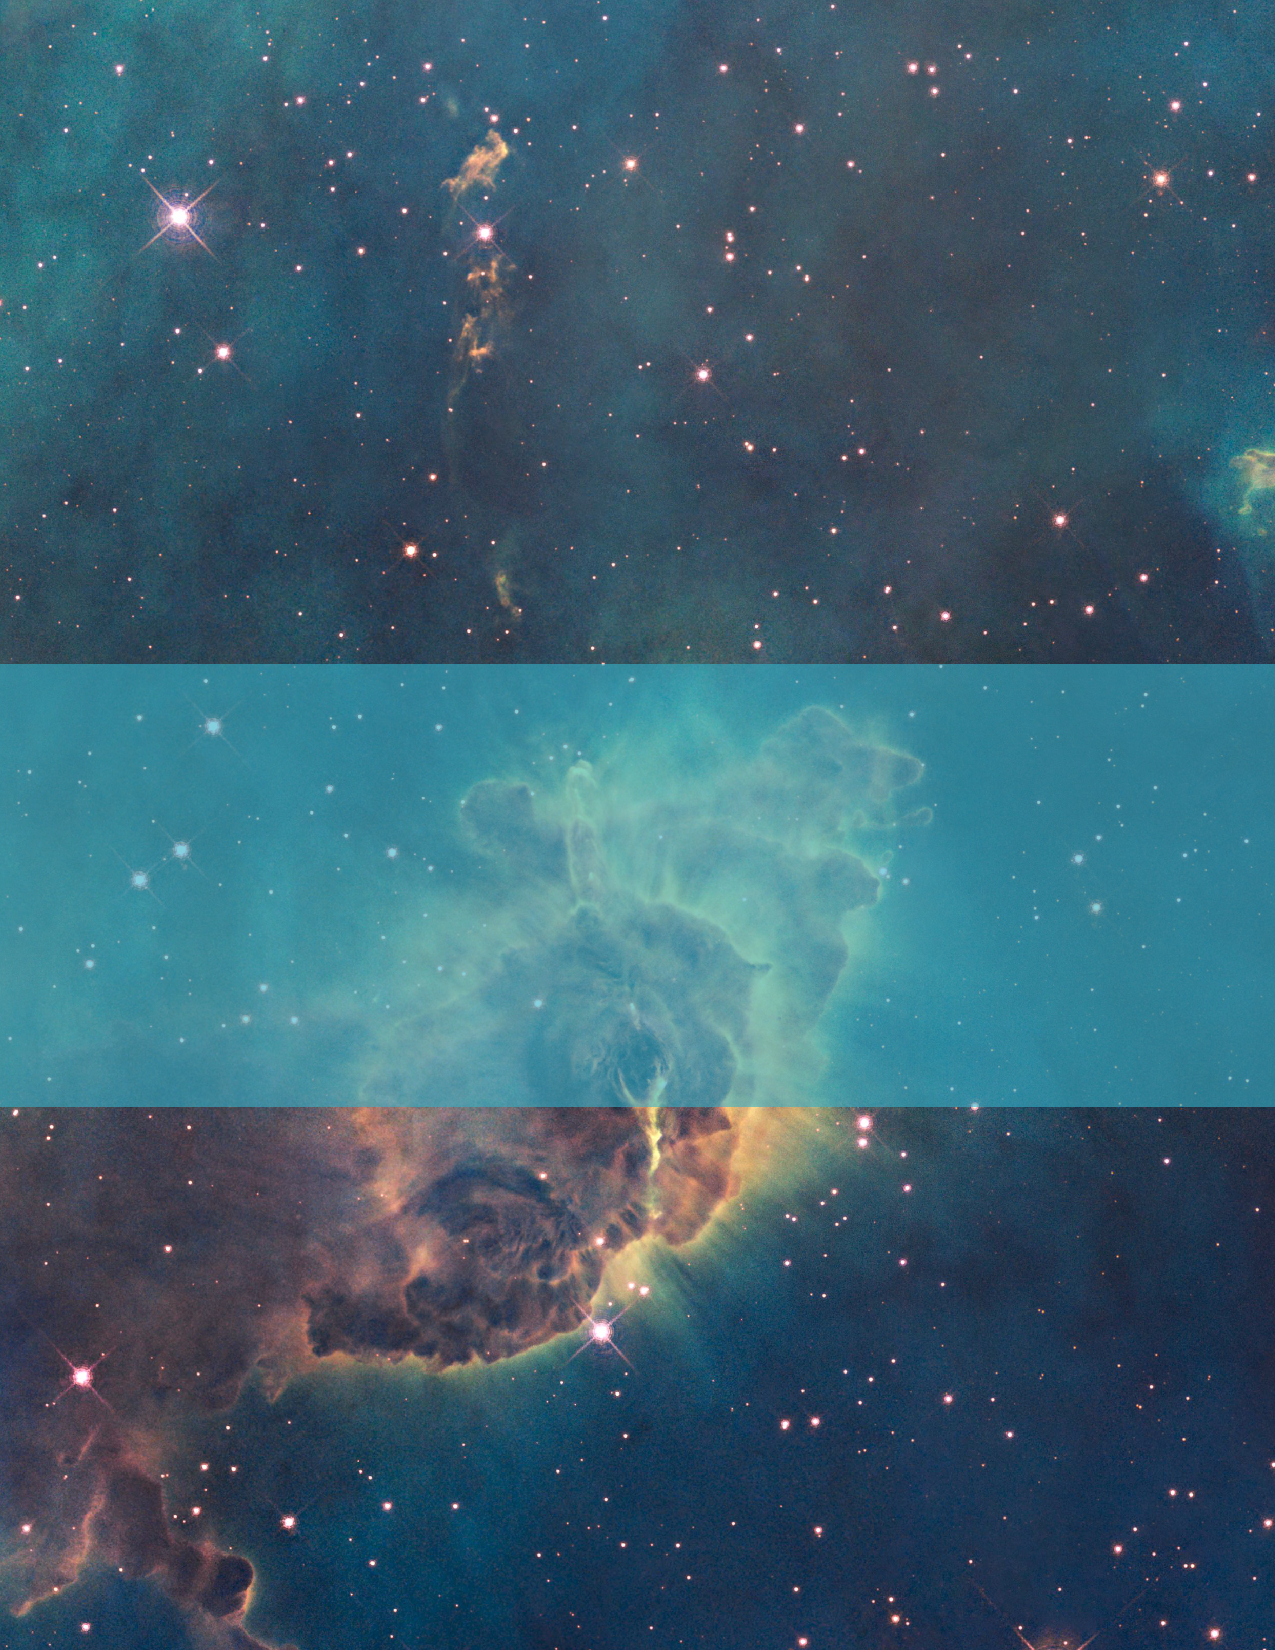
\includegraphics[scale=1.25]{esahubble}}} % Image background
\centering
\vspace*{5cm}
\par\normalfont\fontsize{35}{35}\sffamily\selectfont
{\LARGE High Energy Astrophysics}\par % Book title
\vspace*{1cm}
{\Huge Lecture Notes}\par % Author name
\endgroup

%----------------------------------------------------------------------------------------
%	COPYRIGHT PAGE
%----------------------------------------------------------------------------------------

\newpage
~\vfill
\thispagestyle{empty}

%\noindent Copyright \copyright\ 2014 Andrea Hidalgo\\ % Copyright notice

\noindent \textsc{Eliza Diggins, UC Berkeley}\\

\noindent \textsc{github.com/eliza-diggins}\\ % URL


%----------------------------------------------------------------------------------------
%	TABLE OF CONTENTS
%----------------------------------------------------------------------------------------

\chapterimage{Pictures/high_energy.jpg} % Table of contents heading image

\pagestyle{empty} % No headers

\tableofcontents % Print the table of contents itself

%\cleardoublepage % Forces the first chapter to start on an odd page so it's on the right

\pagestyle{fancy} % Print headers again

%----------------------------------------------------------------------------------------
%	CHAPTER 1
%----------------------------------------------------------------------------------------

\chapterimage{Pictures/high_energy.jpg} % Chapter heading image

\part{Equations And Values}
\clearpage
\newgeometry{left=0.5cm,right=0.5cm,top=0.5cm,bottom=0.8cm}
\thispagestyle{empty}
\fancyhf{}
\renewcommand{\headrulewidth}{0pt}
\begin{center}
{\Large \textbf{Important Constants and Equations}}
\end{center}
\setlength{\abovedisplayskip}{4pt}
\setlength{\belowdisplayskip}{4pt}
\begin{multicols}{2}
\setlength{\columnseprule}{0pt}
\setlength{\columnsep}{0.8cm}

% ----------------------------- %
% CONSTANTS                     %
% ----------------------------- %
\subsection*{Constants}
\footnotesize
\[
\begin{aligned}
  m_p &= 1.67\times10^{-24}\,{\rm g} &
  m_e &= 9.11\times10^{-28}\,{\rm g} \\
  M_\odot &= 1.99\times10^{33}\,{\rm g} &
  R_\odot &= 6.96\times10^{10}\,{\rm cm} \\
  L_\odot &= 3.83\times10^{33}\,{\rm erg\,s^{-1}} \\
  m_p c^2 &= 938\,{\rm MeV} &
  m_e c^2 &= 511\,{\rm keV} \\
  k_B &= 8.62\times10^{-5}\,{\rm eV\,K^{-1}} \\
  \sigma_T &= 6.65\times10^{-25}\,{\rm cm^2} \\
  R_{\rm WD} &\sim 10^9\,{\rm cm} &
  R_{\rm NS} &\sim 10^6\,{\rm cm}
\end{aligned}
\]
\subsection*{Accretion Physics}
\footnotesize
\[
\begin{aligned}
L_{\rm Edd} &= \frac{4\pi G M m_p c}{\sigma_T}
= 1.3\times10^{38}\!\left(\frac{M}{M_\odot}\right)\!{\rm erg\,s^{-1}},\\
L_{\rm acc} &= \frac{GM\dot M}{R} = \eta c^2 \dot{M} = 9\times 10^{36} \;\eta\;\dot{m}_{16}\; {\rm erg\;s^{-1}}\\
&= 5.6\times10^{46}\;\eta \left(\frac{\dot{M}}{1\;{\rm M_\odot\;yr^{-1}}}\right) \;{\rm erg\;s^{-1}}\\
\dot M_{\rm Edd} &= \frac{L_{\rm Edd}}{\eta c^2}
= 1.4\times10^{17}\,\eta^{-1}
\!\left(\frac{M}{M_\odot}\right)\;{\rm g\,s^{-1}}\\
&= 2.2 \times 10^{-9} \eta^{-1} \left(\frac{M}{\rm M_\odot}\right)\; {\rm M_\odot \; yr^{-1}}.
\end{aligned}
\]
\subsubsection*{Bondi Accretion}
\footnotesize
\[
\begin{aligned}
    R_{\rm B} &= \frac{2GM}{c_s^2} = \frac{2GM}{\gamma kT} m_p\mu\\
    &\approx 17.74 \left(\frac{M}{M_\odot}\right) \left(\frac{c_s}{10\;{\rm km\;s^{-1}}}\right)^{-2}\;{\rm AU}.\\
    \dot{M}_{\rm B} &= \pi G^2M^2 \frac{\rho_0}{c_{s,0}^3}\left[\frac{2}{5-3\gamma}\right]^{(5-3\gamma)/2(\gamma-1)}\approx 4\pi G^2M^2 \rho_0c_{s,0}^{-3}\\
    &\approx 3.7\times10^{11} \left(\frac{M}{M_\odot}\right)^2 \left(\frac{c_{s,0}}{10\;{\rm km\;s^{-1}}}\right)^{-3} \left(\frac{\rho_0}{m_p\;{\rm cm^{-3}}}\right) {\rm g\;s^{-1}}
\end{aligned}
\]


\vfill\null\columnbreak

\end{multicols}


\restoregeometry


\part{Fundamentals}

\chapter{Introduction}
High energy astrophysics is, to first order, the study of violent / extreme processes which produce high energy light (X-ray and $\gamma$-ray). In the modern view, this includes things like gravitational radiation, high energy particles, etc. In general, high energy phenomena need to bring together two relevant processes: \textbf{energy generation} and \textbf{energy dissipation}. Generally, high energy processes are driven by a conversion to kinetic energy and then a secondary dissipation into thermal energy.

\section{What Makes High Energy Different}

There are a number of things that distinguish the high energy regime of astrophysics from lower energy regimes. A few relevant ones are
\vspace{0.5cm}
\begin{enumerate}
    \item High energy photons are $\sim 1\; \rm{MeV}$, so for the same energy budget, you can expect to get \textbf{only a fraction as many photons}.
    \item The high energy sky is \textbf{quite}, there are relatively few environments in which you can generate high energy photons. These tend to be point sources,
    although exceptions do exist.
    \item These photons often require some specialized techniques to be stopped.
\end{enumerate}

We also get emission from a large number of different sources, all of which have very different physics and scale very differently:

\begin{table}[htp!]
\centering
\renewcommand{\arraystretch}{1.3}
\begin{tabular}{|p{3cm}|p{3cm}|p{8cm}|}
\hline
\textbf{Energy Range} & \textbf{Thermal Equivalent} & \textbf{Processes Probed} \\
\hline
$E < 10\;\mathrm{keV}$ 
& $T < 10^{8}\;\mathrm{K}$ 
& 
\begin{itemize}
  \item K, L shell line emission ($T \lesssim 5\times 10^{7}\,$K), e.g. iron K$\alpha$ line at 6.4 keV  
  \item Bremsstrahlung (galaxy clusters, SNRs, AGN coronae)  
  \item Blackbody emission
\end{itemize} \\
\hline
$10\;\mathrm{keV} - 10\;\mathrm{MeV}$ 
& typically all atoms fully ionized, electrons stripped 
& 
\begin{itemize}
  \item Isomeric transitions from metastable nuclei  
  \item $\gamma$-ray lines that are nucleosynthetic signatures (e.g. $^{60}$Co $\rightarrow$ $^{60}$Ni + $e^-$ + $\bar{\nu}_e$ + $\gamma$, $E_\gamma \approx 1.1\;\mathrm{MeV}$; SN remnants)  
  \item Radioactive decay: excited nucleus $\rightarrow$ ground state + $\gamma$-ray
\end{itemize} \\
\hline
$E \sim 511\;\mathrm{keV} = m_e c^2$ 
& $T \sim 10^{9}\;\mathrm{K},\; \Gamma \sim 1$ 
& 
\begin{itemize}
  \item $e^+ e^-$ annihilation lines: $e^+ + e^- \rightarrow \gamma + \gamma$
\end{itemize} \\
\hline
$140\;\mathrm{MeV} - 10\;\mathrm{GeV}$ 
& $T \sim 10^{12}\;\mathrm{K},\; \Gamma \sim 1000$ (up to $10^{6}$) 
& 
\begin{itemize}
  \item Pion mass scale (strong force $\rightarrow$ hadrons)  
  \item Baryons ($uud$, $udd$; 3 quarks)  
  \item Mesons ($u\bar{d}$, etc.; 2 quarks, includes pions)
\end{itemize} \\
\hline
$E > 10\;\mathrm{GeV}$ 
& $\Gamma > 10^{6}$ 
& 
\begin{itemize}
  \item Non-thermal processes:  
  \begin{itemize}
    \item Inverse Compton scattering  
    \item Particle acceleration
  \end{itemize}
\end{itemize} \\
\hline
\end{tabular}
\caption{Physics probed at different photon energies.}
\end{table}


\section{Where Does the Energy Come From}

There are 3 major processes which produce the energy that drives high energy phenomena:
\vspace{0.5cm}
\begin{enumerate}
    \item \textbf{Gravitational Energy:}  
    In high-energy astrophysics, gravitation is the dominant source of kinetic energy. Material falling in a gravitational potential well is accelerated to high velocities; this energy is then thermalized and radiated.  

    For a uniform-density sphere, the total gravitational binding energy is
    \[
        U = -\frac{3}{5}\frac{GM^2}{R}.
    \]
    The characteristic \textit{specific energy} (energy per unit mass) is therefore
    \[
        \tilde{u} \sim \frac{GM}{R}.
    \]
    In cgs units, this scales as
    \[
        \tilde{u} \approx 1.9 \times 10^{15}
        \left(\frac{M}{M_\odot}\right)
        \left(\frac{R}{R_\odot}\right)^{-1}
        \;\mathrm{\frac{erg}{g}}.
    \]
    \begin{remark}
        One thing to keep in mind is that of these three, gravitation is the only one that is decidedly variable. For instance, in a stellar system, we have around $10^{15}\;{\rm erg \;g^{-1}}$, but in a highly compact system $(GM/R \sim 1)$, we have instead $10^{21}\;{\rm erg\;g^{-1}}$.
    \end{remark}
    \item \textbf{Nuclear Energy:}  
    Nuclear fusion reactions in stellar cores release $\sim 1\;\mathrm{MeV}$ per baryon, corresponding to a specific energy of order
    \[
        \tilde{u}_{\rm nuc} \sim 10^{18}\;\mathrm{\frac{erg}{g}}.
    \]

    \item \textbf{Chemical Energy:}  
    Chemical reactions typically release energy on the $\sim 1\;\mathrm{eV}$ per baryon scale, giving a specific energy of order
    \[
        \tilde{u}_{\rm chem} \sim 10^{13}\;\mathrm{\frac{erg}{g}}.
    \]
\end{enumerate}

\section{How is the Energy Dissipated?}

Regardless of the initial source, high energy phenomena leave us with many particles moving at extreme velocities. To produce the observable high-energy radiation, this kinetic energy must be \textbf{thermalized} or otherwise converted into photon emission. There are three major dissipation channels:

\begin{itemize}
    \item \textbf{Shocks:}  
    When supersonic flows collide, they form shock fronts. Shocks provide an efficient way to convert bulk kinetic energy into random particle motion. In astrophysics, strong shocks are ubiquitous --- e.g.\ supernova remnants, accretion flows, and jets --- and they often accelerate particles to non-thermal distributions (Fermi acceleration).

    \item \textbf{Viscous Dissipation:}  
    Even in the absence of strong shocks, turbulent or shearing flows can gradually convert bulk kinetic energy into thermal energy through viscosity. In astrophysical plasmas the ``viscosity'' is often anomalous, mediated by small-scale instabilities and wave–particle interactions (rather than molecular collisions). This mechanism is critical in accretion disks.

    \item \textbf{Magnetic Fields:}  
    Magnetized plasmas store and redistribute energy through magnetic tension and reconnection. Magnetic reconnection events rapidly convert magnetic energy into particle kinetic energy and heat, often producing non-thermal particle populations (e.g.\ solar flares, pulsar magnetospheres). Synchrotron and inverse-Compton processes then radiate this energy efficiently.
\end{itemize}

\chapter{Radiative Processes}
In this chapter, we will review some of the critical elements of radiative transfer and radiative processes. These can be found more thoroughly treated in \textit{Rybicki \& Lightman} among others.

\section{Intensity and Other Definitions}

To begin, we need to clarify some definitions that are commonly used. We begin with \textbf{specific intensity}:
\vspace{0.5cm}
\begin{definition}[Specific Intensity]
The \textbf{specific intensity} $I_\nu(\mathbf{x}, \hat{\mathbf{n}}, t)$
is the energy transported by radiation per unit area, per unit time, per
unit frequency, per unit solid angle:
\[
    I_\nu \;\; \left[ \frac{\mathrm{erg}}
                          {\mathrm{s}\,\mathrm{cm}^2\,
                           \mathrm{Hz}\,\mathrm{sr}} \right].
\]
Formally,
\[
    dE = I_\nu \cos\theta \; dA \; dt \; d\nu \; d\Omega,
\]
where $\theta$ is the angle between $\hat{\mathbf{n}}$ (the propagation
direction) and the surface normal $dA$. \rmk{You can also write this with a dot product and $d{\bf A}$.}
\end{definition}
\vspace{0.5cm}
We are also quite interested in various \textbf{moments} of $I_\nu$ in order to generate other useful quantities:
\vspace{0.25cm}
\begin{definition}[Mean Intensity]
The \textbf{mean intensity} is the angle average of the specific
intensity:
\[
    J_\nu = \frac{1}{4\pi}\int I_\nu(\hat{\mathbf{n}})\, d\Omega,
    \qquad
    J_\nu \;\; \left[ \frac{\mathrm{erg}}
                          {\mathrm{s}\,\mathrm{cm}^2\,
                           \mathrm{Hz}\,\mathrm{sr}} \right].
\]
This quantity is isotropic by construction. It effectively counts the number of photons arriving at a point in space regardless of the direction.
\end{definition}
\vspace{0.25cm}
The \textbf{flux} is another common quantity, which ends up being the \textbf{first moment} of the specific intensity. Whereas intensity tells us how much energy we get from a particular direction, \textbf{flux tells us the total energy transfer from all directions}. Formally, we define the \textbf{flux vector} as
\vspace{0.25cm}
\begin{definition}[Flux]
    For a radiation field with specific intensity $I_\nu({\bf x},t, \hat{\bf n})$, the \textbf{flux vector} is 
\begin{equation}
        \boxed{
    {\bf F}_\nu = \int_{4\pi} I_\nu({\bf x},t,\hat{\bf n}) \hat{\bf n} \; d\Omega.
    }
\end{equation}
    If we then consider the quantity of energy passing through a surface $d{\bf A}$ in a unit time,
    \[
    dE_{\perp} = \int_{4\pi} d\Omega \; I_\nu (\hat{\bf n} \cdot d{\bf A}) = {\bf F}_\nu \cdot d{\bf A} = F_\nu \cos\theta dA.
    \]
\end{definition}

The first of these definitions encodes the direction of energy transfer, while the second describes how energy transfer occurs through a specific surface.
\par
We also distinguish between $\nu$-specific quantities and quantities integrated over $\nu$.
\vspace{0.25cm}
\begin{definition}[Bolometric vs. Monochromatic]
A \textbf{monochromatic} quantity is specified at a fixed frequency
$\nu$; for example, $I_\nu$ or $F_\nu$.  
A \textbf{bolometric} quantity is integrated over frequency:
\[
    I = \int_0^\infty I_\nu \, d\nu,
    \qquad
    F = \int_0^\infty F_\nu \, d\nu.
\]
Bolometric quantities therefore have units without the ``per Hz'' factor.
\end{definition}

\begin{definition}[Luminosity]
The \textbf{monochromatic luminosity} $L_\nu$ is the total power emitted
by a source per unit frequency:
\[
    L_\nu = \int_{\partial V} F_\nu \, dA,
    \qquad
    L_\nu \;\; \left[ \frac{\mathrm{erg}}
                          {\mathrm{s}\,\mathrm{Hz}} \right].
\]
The \textbf{bolometric luminosity} is
\[
    L = \int_0^\infty L_\nu \, d\nu
      = \int_{\partial V} F \, dA,
    \qquad
    L \;\; \left[ \frac{\mathrm{erg}}{\mathrm{s}} \right].
\]
\end{definition}
\par
The final integral over $I_\nu$ worth mentioning is the \textbf{energy density of radiation}:
Imagine that you hold a metal shield up to the sky in direction $\hat{\bf n}$. In some $dt$, a cone of photons will hit that shield. That cone of photons will have infinitesimal volume $c \; \cos \theta \;dAdt$. \rmk{the $\cos$ comes in because different cones see different cross sections.} Now, we know that the resulting energy that arrives at the shield is
\[
\delta E = I_\nu({\bf x},\hat{\bf n}) (\hat{\bf n} \cdot d{\bf A}) d\Omega d\nu dt.
\]
Within that region, there was
\[
u_\nu dV d\Omega d\nu
\]
energy, so setting these equal to one another,
\[
u_\nu(\hat{\bf n}) = \frac{1}{c} I_\nu({\bf x},\hat{\bf n}).
\]
If we integrate over all directions, we have
\begin{equation}
    \boxed{
    u_\nu = \frac{1}{c}\int_{4 \pi} I_\nu \;d\Omega = \frac{4\pi}{c} J_\nu,
    }
\end{equation}
where $J_\nu$ is the \textbf{average intensity}.


\section{Radiative Transfer}

Consider two disks a distance $dx$ apart with areas $dA_i$. Now, we are interested in the energy transfer of rays which pass through both screens. Consider first screen 1. A ray passing through screen one must be directed such that it points in the right direction to hit screen two, which has angular area $dA_2/dx^2$. Thus, the energy transfered along those rays is
\[
dE = I_{\nu,1} \;dA_1 dt d\Omega d\nu = I_{\nu,1} \frac{dA_1 dA_2}{dx^2} dt d\nu.
\]
Likewise, at screen 2, only those photons which passed through angular area $dA_1/dx^2$ could have passed through both, so
\[
dE = I_{\nu,2} \; dA_2 dt d\Omega d\nu \implies I_{\nu,1} = I_{\nu,2}.
\]
Thus, \textbf{intensity is conserved along rays}.
\par
There is however a caveat to this:

\begin{itemize}
    \item Light can be \textbf{scattered into a ray},
    \item Light can also be \textbf{emitted / absorbed} into a ray.
\end{itemize}

As such, there are some scenarios in which intensity along a ray is not constant.

\subsection{Emission}

Let's determine some of the nomenclature for emission mechanics. We define the \textbf{spontaneous emission coefficient} such that
\vspace{0.5cm}
\begin{definition}[Spontaneous Emission Coefficient]
\label{def:spont_emission_coef}
The \textbf{spontaneous emission coefficient} is the energy injected / emitted per unit time, per unit solid angle, and per unit volume. Thus
\[
dE = j(t,\hat{\bf n})\; dV d\Omega dt.
\]
\rmk{Note that this means the coefficient is a function of direction. This is the case for (say) Larmor radiation, which is not isotropic.}
\par
This can likewise be defined in terms of a \textbf{monochromatic emission coefficient} $j_\nu$, which is just the emission per unit frequency as well. Likewise, for \textbf{isotropic emission}, 
\[
dE = \int_{4\pi} d\Omega\; j_\nu dV dt = 4\pi j_\nu \; dV dt.
\]
Thus,
\[
P_\nu = \frac{j_\nu}{4\pi}
\]
is the \textbf{monochromatic power per unit volume.}
\end{definition}
\vspace{0.5cm}
We also often define another useful quantity which occurs in the context of \textbf{isotropic emission}:
\begin{definition}[Emissivity]
\
    The \textbf{emissivity} is the energy emitted per unit frequency, per unit mass, per unit time. It is thus \textbf{angle integrated}. Formally,
    \[
    dE = \epsilon_\nu \rho \; dV dt d\nu \frac{d\Omega}{4\pi}.
    \]
\end{definition}
\vspace{0.5cm}
By comparison to $j_\nu$, we see that 
\[
j_\nu = \frac{\epsilon_\nu \rho}{4\pi}.
\]
\paragraph{Added Intensity}
Having worked out all the definitions above, we want to know what the change in $dI_\nu$ is for a particular path $ds$. For an isotropic emitter,
\begin{equation}
\label{eq:emit_coeff}
    \boxed{
dI_\nu = j_\nu ds.
}
\end{equation}

\subsection{Absorption}
Unlike emission, where we are generally more interested in energy generation that we are in intensity specifically, for absorption, we simply \textit{define} absorption on the basis of decreasing intensity. Formally,
\vspace{0.5cm}
\begin{definition}[Absorption Coefficient]
The \textbf{absorption coefficient} is defined such that
\begin{equation}
\label{eq:absorb_coef}
\boxed{
    dI_\nu = -\alpha_\nu I_\nu ds.
    }
\end{equation}
Thus, it is the loss per unit intensity per unit length. 
\end{definition}
\vspace{0.5cm}
Now, it is generally good practice to connect $\alpha$ to a theoretical statement about the absorbers in question. Consider that a ray passes through an ambient space with a number density $n$ of absorbing particles, each of which has effective area $\sigma$. In a cylindrical region with area $dA$ and length $ds$, there are clearly $n \;dAds$ absorbers along the line of sight. Assuming that they are small enough that overlaps are unlikely, this would obscure some $n \sigma_\nu \; dAds$ of the available aperature. Now, \textbf{those particles absorb energy}:
\[
- dE = I_\nu \; dA_{\rm absorption}\;dt\;d\Omega\;d\nu = I_\nu (n \sigma_\nu dA dS) dt d\Omega d\nu.
\]
The intensity will also change because 
\[
-\Delta dE = - \Delta dI_\nu dA d\Omega dt d\nu = I_\nu (n\sigma_\nu dAds) dtd\omega d\nu.
\]
Cancelling terms, we find
\[
dI_\nu = -n\sigma_\nu I_\nu ds,
\]
so
\[
\boxed{
\alpha=n\sigma_\nu = \rho \kappa_\nu,
}
\]
where $\kappa$ is the \textbf{opacity.}
\begin{remark}
    One needs to be careful that this is valid since we require $\sigma_\nu^{1/2} \ll n^{-1/3}$ in order to not have issues with overlap and we also assume random distribution. This is \textbf{almost always the case}. Additionally, some things like stimulated emission are actually treated as part of the absorption since they are proportional to the intensity nonetheless.
\end{remark}
\subsection{The Equations of Radiative Transfer}

If we combine equations~\ref{eq:absorb_coef} and \ref{eq:emit_coeff}, we find the \textbf{classical radiative transfer equation}:
\begin{equation}
    \label{eq:radiative_transfer}
    \frac{dI_\nu}{ds} = -\alpha_\nu I_\nu + j_\nu.
\end{equation}
There are two special cases to consider before generating a fully formalized solution to the above equation:

\subsubsection*{Emission Only}
If the scenario without any absorption, we have $\alpha = 0$, so
\[
\boxed{
\frac{dI_\nu}{ds} = j_\nu \implies I_\nu = I_{\nu0} + \int_0^s j_\nu(\xi) \;d\xi.
}
\]
\rmk{So the increase in brightness is just the integral of the emission coefficient along the LOS.}
\subsubsection*{Absorption Only}
This one is a little trickier. We have
\[
\frac{dI_\nu}{ds} = -\alpha I_\nu.
\]
Formally, we have
\[
I_\nu(s) = I_\nu(0) \exp\left[-\int_0^s \alpha_\nu(\xi)\;d\xi\right].
\]
We may; however, make this solution somewhat simpler by introducing a \textit{dimensionless length scale}. We therefore introduce $d\tau = \alpha ds$ which then means that
\[
d\log I_\nu = -d\tau \implies I_\nu(\tau) = I_\nu(0) e^{-\tau},
\]
where we have implicitly set $\tau$ to be zero at our starting point. Formally,
\begin{equation}
    \label{eq:optical_depth}
    \boxed{
    \tau_\nu(s) = \int_0^s d\xi\; \alpha_\nu(\xi).
    }
\end{equation}
Now, if $I_\nu \propto \exp(-\tau)$, then we see that for $\tau \ll 1$, we have very little drop off and (for this particular sight line), the medium is \textbf{transparent}. Likewise, if $\tau \gg 1$, then it is \textbf{optically-thick} or \textbf{opaque.}

\subsubsection*{The Formal Solution}
Let's return to
\[
\frac{dI_\nu}{ds} = -\alpha_\nu I_\nu + j_\nu.
\]
in the $\tau$ coordinate system,
\[
\frac{1}{\alpha_\nu} \frac{dI_\nu}{ds} = \frac{dI_\nu}{d\tau} = -I_\nu + S_\nu,
\]
where $S_\nu = j_\nu/\alpha_\nu$ is the \textbf{source term}. Now, this may be solved by an integrating factor, so
\[
\left(\frac{dI_\nu}{d\tau} + I_\nu\right)e^\tau = \frac{d}{d\tau} \left(e^\tau I_\nu\right) = e^\tau S_\nu.
\]
As such,
\[
e^\tau I_\nu = I_\nu(0) +\int_0^\tau d\xi \;S_\nu(\xi) e^\xi, 
\]
so
\[
\boxed{
I_\nu(\tau) = I_{\nu,0}e^{-\tau} + \int_0^\tau d\xi \; S_\nu(\xi) e^{\xi-\tau}.
}
\]
\subsection{The Mean Free Path}

In a medium with \textbf{no sources}, the equation above suggests that
\[
I_\nu(\tau) = I_{\nu,0} e^{-\tau}.
\]
Since the intensity encodes the number of photons effectively passing through a region, we see that
\[
P_{\rm collision} = \frac{I_\nu}{I_{\nu,0}} = e^{-\tau}.
\]
We can then ask what the average distance before collision will be. Clearly,
\[
\left<\tau\right> = \int_0^\infty \tau e^{-\tau} d\tau = 1 \implies \left<\ell\right> = (1/\alpha_\nu) = 1/(n\sigma_\nu).
\]
This quantity is then the \textbf{mean free path} of the photons between collisions.

\subsection{Radiation Force}
We have already discussed the advent of radiation pressure in a photon gas. We also need to acknowledge that when photons are absorbed in a particular ray, they will experience a force. Recall that the energy flux vector is
\[
{\bf F}_\nu = \int I_\nu \hat{\bf n} \;d\Omega.
\]
Thus,
\[
\frac{d{\bf F}_\nu}{d\tau} = \int \frac{\partial I_\nu}{\partial \tau} \hat{\bf n}\; d\Omega = - \int I_\nu \hat{\bf n} \;d\Omega = -{\bf F}_\nu. 
\]
\rmk{This makes NO SENSE except when you realize $d\tau = \alpha ds$, so if there is no absorption, your parameter doesn't even progress.} We can also write this as 
\[
\frac{d{\bf F}_\nu}{ds} = -\alpha {\bf F_\nu} \implies \frac{d{\bf p}_\nu}{ds} = -\frac{\alpha}{c} {\bf F}_\nu.
\]
Now, this is the \textbf{momentum}, but it is per unit area and per unit path length. But that's just \textbf{momentum density}. We can therefore identify the \textbf{force per unit mass} to be
\[
{\bf f} = \frac{1}{c} \int \kappa_\nu {\bf F}_\nu \;d\nu.
\]

\section{Thermal Radiation}

In this section we study the properties of emission from \textbf{thermally equilibrated material}. 

\subsection{Kirchhoff's Law}

Our first step is to understand how the notion of \textbf{local thermal equilibrium} (LTE) constrains the interaction of matter with radiation. This will lead us to two results collectively known as \textbf{Kirchhoff's Law}. 

\begin{center}
    Imagine a chamber filled with a \textbf{photon gas} in thermal equilibrium at temperature $T$. Now place this chamber in contact with another chamber, also at temperature $T$, but whose walls are made of material that can absorb and emit radiation.
\end{center}

If, at some frequency $\nu$, the two chambers had different intensities $I_{\nu,1} \neq I_{\nu,2}$, there would be a net transfer of photons at that frequency. This would imply a net flow of energy between two systems at the same temperature, in violation of the second law of thermodynamics. Therefore, microscopic absorption and emission must balance in such a way that the radiation field is not disturbed. 

\begin{theorem}[Kirchhoff's Law \#1]
For material in local thermal equilibrium at temperature $T$, the ratio of the emission coefficient to the absorption coefficient is universal and equals the Planck function:
\[
\frac{j_\nu}{\alpha_\nu} = B_\nu(T),
\]
Equivalently, the source function
\[
S_\nu \;\equiv\; \frac{j_\nu}{\alpha_\nu}
\]
is equal to the blackbody intensity at temperature $T$.
\end{theorem}

\begin{remark}
There is an important distinction between \emph{blackbody radiation} and \emph{thermal emission}. 
\begin{itemize}
    \item In a closed cavity where both matter and radiation are in \textbf{global equilibrium}, the radiation field itself must be Planckian:
    \[
    I_\nu = B_\nu(T), \qquad S_\nu = B_\nu(T).
    \]
    This is the defining property of blackbody radiation. 

    \item In contrast, in many astrophysical systems (e.g. stellar atmospheres), the material may be in LTE while the radiation field is not. In this case we still have
    \[
    S_\nu = B_\nu(T),
    \]
    but the actual intensity $I_\nu$ is determined by solving the radiative transfer equation with this source function and the boundary conditions. In general,
    \[
    I_\nu \neq B_\nu(T).
    \]
\end{itemize}
Thus, Kirchhoff's law fixes the form of the \emph{source function}, but only in global equilibrium does the radiation field itself become blackbody.
\end{remark}
\subsection{The Planck Distribution}
We may now endeavor to understand this $B_\nu(T)$ that we have such need of. This will lead us to the \textbf{plank distribution}, which is derived from statistical mechanics. The \textbf{photon gas} has the distinctive property that it is composed of a set of effectively non-interacting bosons. As such, each quantum state is \textbf{independently equilibrated}. A state may therefore have energy $\mathcal{E}$ and $N$ particles within it and can exchange both of these quantities with the rest of the environment. This is therefore a \textbf{grand-canonical ensemble}. The partition function is
\[
\mathcal{Z} = \sum_N \exp(N(\mu - \mathcal{E})\beta).
\]
Now, because these are bosons, there is no upper limit on $N$ as we have for fermions, so we can simply sum this as a geometric series.
\[
\mathcal{Z} = \frac{1}{1-\exp\left[(\mu - \mathcal{E})\beta\right]}.
\]
For photons, the chemical potential is $\mu = 0$, and so the mean occupation of a single mode is
\[
\left<N\right> = \frac{1}{1-\exp(h\nu \beta)}
\]
Now, the question becomes how many modes are there in a particular volume? We characterize a mode by ${\bf n} = (n_1,n_2,n_3)$ and recall that
\[
\mathcal{E} = \frac{hc}{2L} |{\bf n}| \implies d\mathcal{E} = \frac{hc}{2L} dn.
\]
If the density of states $g(\nu)$ is known, then 
\[
g(\nu) d \nu = \pi n^2 dn = \frac{8\pi L^3}{h^3c^3} \mathcal{E}^2 d\mathcal{E} = \frac{8\pi L^3}{c^3} \nu^2 d\nu.
\]
Combining this with the occupation probability yields
\begin{equation}
    \label{eq:bb_radiance}
    \boxed{
    B_\nu(T) = I_\nu(T) = \frac{c}{4\pi} u_\nu(T) = \frac{2 h \nu^3}{c^2} \frac{1}{e^{h\nu/k_bT} -1}.
}
\end{equation}
\subsubsection{Properties of the Plank Distribution}

Here we summarize some critical results from the Plank Distribution:
\vspace{0.25cm}
\begin{definition}[Rayleigh-Jeans Law]
For $h\nu \ll k_bT$, 

\begin{equation}
\label{eq:Rayleigh-Jeans}
\boxed{
I_\nu(T) =  \frac{2\nu^2}{c^2} kT.
}
\end{equation}
\end{definition}
\begin{proof}
    For $h\nu \ll k_bT$, $\exp(h\nu/k_bT) \approx 1+ (h\nu/k_bT)$, so we find the above result.
\end{proof}
\begin{remark}
    This is very useful for a couple of reasons. First off, it allows you to recover Planck if you remember how RJ comes about and how the exponential term should look. Secondly, for \textbf{low frequency radiation}, this approximation is almost always legitimate and is linear in $\nu$.
\end{remark}
\vspace{0.25cm}
In the \textbf{high frequency limit}, we have an equivalent result called \textbf{Wein's Law}:
\vspace{0.25cm}
\begin{definition}[Wein's Law]
    For $h\nu \gg k_bT$, we have
    \begin{equation}
        \label{eq:Wein-Law}
            I_\nu(T) = \frac{2h \nu^3}{c^2} \exp\left(\frac{-h\nu}{kT}\right).
    \end{equation}
\end{definition}
\vspace{0.25cm}
We also have the following two useful propositions:
\vspace{0.1cm}
\begin{proposition}[Monotonicity]
Let $T_1$ and $T_2$ be temperatures. $T_1 > T_2$ implies that $I_\nu(T_1) > I_\nu(T_2)$ for all $\nu$.
\end{proposition}
\begin{proof}
    This is done simply by taking the derivative with respect to $T$ and showing that it is always positive.
\end{proof}

\begin{proposition}[Wein's Offset Law]
The \textbf{peak frequency} $\nu_{\rm max}$ is such that
\[
h\nu_{\rm max} = 2.82\; kT.
\]
\end{proposition}

\subsection{Thermodynamics of BB Radiation}
As we have previously discussed, emission and absorption from the barriers of the container can serve to thermalize light into a blackbody spectrum. If we then compress or expand the cavity, we have thermodynamic work from which we can gain great insight. First off
\[
dU = TdS - pdV \implies dS = \frac{1}{T}dU + \frac{p}{T} dV.
\]
We know, however, that $p = u/3$ from arguments made about the photon gas, and we know that $U=u(T) V$, so
\[
dS = \frac{1}{T}\left[u dV + Vdu\right] + \frac{1}{3}\frac{u}{T} dV =\frac{4}{3} \frac{u}{T} dV + \frac{V}{T}du.
\]
now, $S$ is a function of $T$ and $V$, so
\[
ds = \left(\frac{\partial u}{\partial T}\right)_V dT + \left(\frac{\partial u}{\partial V}\right)_T dV.
\]
As such,
\[
\frac{\partial^2 S}{\partial T \partial V} = -\frac{4}{3}\frac{u}{T^2} + \frac{4}{3} \frac{1}{T} \frac{\partial u}{\partial T} =  \frac{1}{T}\frac{du}{dT}.
\]
The result is that
\[
\frac{du}{u} = 4 \frac{dT}{T} \implies \log u = 4 \log T +\log a.
\]
This is the \textbf{steffan-Boltzmann Law}:
\[
u(T) = aT^4,
\]
where $a$ is the \textbf{radiation constant}. We may likewise calculate the \textbf{flux} as
\[
F = \sigma T^4.
\]

\subsection{Characteristic Temperatures}

Several characteristic temperatures are defined in relation to thermal emission.  
They allow us to compare real sources with the idealized behavior of a blackbody.

\vspace{0.5cm}
\begin{definition}[Brightness Temperature]
The \textbf{brightness temperature} $T_b(\nu)$ is the temperature a blackbody would need to have in order to produce the same specific intensity at a given frequency $\nu$:
\[
I_\nu = B_\nu\!\left(T_b(\nu)\right).
\]
Since the definition is frequency–dependent, $T_b$ is in general a function of $\nu$.
\end{definition}

\vspace{0.3cm}
\begin{definition}[Color Temperature]
The \textbf{color temperature} $T_c$ is the temperature of a blackbody whose spectrum peaks at the same frequency (or wavelength) as the observed source, i.e.
\[
\nu_{\rm max}^{\rm source} = \nu_{\rm max}^{\rm BB}(T_c).
\]
\end{definition}

\vspace{0.3cm}
\begin{definition}[Effective Temperature]
The \textbf{effective temperature} $T_{\rm eff}$ is the temperature of a blackbody that would produce the same total flux as the source.  
For a source with bolometric flux $F$,
\[
F = \int I_\nu \cos\theta \, d\Omega \, d\nu = \sigma T_{\rm eff}^4.
\]
\end{definition}
\par
There are a few remarks worth making about these temperature measures:
\vspace{0.2cm}
\begin{itemize}
    \item \textbf{Brightness temperature $T_b(\nu)$.}  
    In the radio regime, the Rayleigh–Jeans approximation to the Planck function applies:
    \[
    B_\nu(T) \approx \frac{2\nu^2 k_B T}{c^2}.
    \]
    Using the definition $I_\nu = B_\nu(T_b)$, this gives
    \[
    T_b(\nu) \;\approx\; \frac{c^2}{2k_B \nu^2} I_\nu.
    \]
    Thus, $T_b$ can be obtained directly from a measured intensity $I_\nu$ by a simple algebraic inversion.  
    This is one of the main reasons $T_b$ is widely used in radio astronomy.
    
    \item \textbf{Color temperature $T_c$.}  
    $T_c$ depends only on the \emph{shape} of the spectrum, since it is defined by the location of the emission maximum.  
    For a blackbody, Wien’s displacement law gives
    \[
    \nu_{\rm max} \propto T_c, \qquad \lambda_{\rm max} T_c = b,
    \]
    with $b \approx 2.9 \times 10^{-3}\,\mathrm{m \, K}$.  
    Because the peak is a function of spectral shape alone, $T_c$ is insensitive to the overall flux normalization.

    \item \textbf{Effective temperature $T_{\rm eff}$.}  
    $T_{\rm eff}$ encodes the total radiated power, independent of spectral details.  
    For a source of luminosity $L$ and radius $R$,
    \[
    F = \frac{L}{4\pi R^2} = \sigma T_{\rm eff}^4,
    \]
    where $F$ is the bolometric flux at the surface.  
    This makes $T_{\rm eff}$ the standard measure for stellar classification and energy output.
\end{itemize}

\section{Electron Scattering}

In this section, we briefly touch on the details of \textbf{Thompson scattering} and its relativistic counterpart \textbf{Compton scattering}. 

\subsection{Thompson Scattering}

\begin{definition}[Thomson Scattering]
    \label{def:thomson_scattering}
    \textbf{Thomson scattering} is the non--relativistic limit of the
    scattering of an incident electromagnetic wave off of a free
    electron.
\end{definition}

\noindent
Consider an incident plane electromagnetic wave,
\[
    {\bf E}({\bf x},t) = E_0 \exp\!\left[i({\bf k}\cdot{\bf x} - \omega t)\right]\boldsymbol{\epsilon},
\]
where $\boldsymbol{\epsilon}$ is the polarization vector of the incoming
wave. In the non--relativistic limit ($\beta \ll 1$), the Lorentz force
reduces to
\[
    {\bf F}_{\rm Lorentz} = q\left({\bf E} + \frac{\mathbf{v}}{c}\times {\bf B}\right)
    \approx q{\bf E},
\]
so that the electron’s equation of motion is
\[
    m\ddot{\bf r} = q{\bf E} \qquad \implies \qquad
    \ddot{\bf d} = \frac{q^2}{m}{\bf E},
\]
where ${\bf d} = q{\bf r}$ is the electric dipole moment of the electron.
Integrating twice gives
\[
    {\bf d}(t) = -\frac{q^2}{m\omega^2}{\bf E}(t),
\]
so the electron behaves as an oscillating dipole of frequency $\omega$
and amplitude
\[
    {\bf d}_0 = \frac{q^2E_0}{m\omega^2}\,\boldsymbol{\epsilon}.
\]
\begin{remark}
    The dipole oscillation is \textbf{coherent} with the polarization of
    the incident wave: the electron is driven along
    $\boldsymbol{\epsilon}$.
\end{remark}

\noindent
For a sinusoidal oscillation ${\bf d}(t) \propto \sin(\omega t)$, the
angular distribution of radiated power follows from the dipole formula:
\[
    \frac{dP}{d\Omega} = \frac{q^4E_0^2}{8\pi m^2 c^3}\,\sin^2\theta.
\]
To connect this with scattering, we compare with the definition
\[
    \frac{dP}{d\Omega} = \langle {\bf S} \rangle \frac{d\sigma}{d\Omega},
\]
where $\langle {\bf S} \rangle$ is the time--averaged incident flux.
This yields the polarized differential cross section
\[
    \frac{d\sigma}{d\Omega} = r_0^2 \sin^2\theta,
\]
where
\[
    r_0 \equiv \frac{q^2}{mc^2}
\]
is the \textbf{classical electron radius}. An equivalent view of the cross section is that
for a given incident polarization vector $\boldsymbol{\epsilon}$, the radiated dipole field is proportional to the projection of
$\boldsymbol{\epsilon}$ onto directions transverse to the outgoing wave vector $\hat{\mathbf{n}}$. The polarized differential cross section can
therefore be written in the coordinate--free form
\[
    \frac{d\sigma}{d\Omega} = r_0^2 \, |\hat{\boldsymbol{\epsilon}} \cdot \hat{\boldsymbol{\epsilon}}'|^2,
\]
where $\hat{\boldsymbol{\epsilon}}'$ is the unit polarization vector of the scattered wave (necessarily perpendicular to $\hat{\mathbf{n}}$).
For the special case of an incident wave along the $z$--axis with polarization along $x$, this reduces to the familiar
\[
    \frac{d\sigma}{d\Omega} = r_0^2 \sin^2\theta.
\]
If the incident light is unpolarized, we average over two orthogonal polarizations of the incoming wave. This eliminates the dependence on the polarization orientation, leaving a distribution that depends only
on the scattering angle:
\[
    \left(\frac{d\sigma}{d\Omega}\right)_{\rm unpol}
    = \tfrac{1}{2} r_0^2 \big(1 + \cos^2\theta\big).
\]
This is the standard angular dependence of Thomson scattering for unpolarized radiation. Integrating the unpolarized expression over solid angle yields
\begin{equation}
    \label{eq:thomson_cross_section}
    \boxed{\sigma = \frac{8\pi}{3} r_0^2.}
\end{equation}
For electrons, this evaluates to the classic \textbf{Thomson cross
section},
\[
    \sigma_T \simeq 6.65 \times 10^{-25}\;\mathrm{cm}^2.
\]

\begin{remark}
    \textbf{Key Points:}
    \begin{enumerate}
        \item \emph{Forward--Backward Symmetry:}  
              The unpolarized differential cross section
              \[
                  \left(\frac{d\sigma}{d\Omega}\right)_{\rm unpol}
                  = \tfrac{1}{2} r_0^2 (1 + \cos^2\theta)
              \]
              is symmetric under $\theta \to \pi - \theta$. This means
              that scattering into a given forward angle is just as
              likely as into the corresponding backward angle. In
              Thomson scattering there is no intrinsic preference for
              forward or backward scattering.

        \item \emph{Total Cross Section Independence:}  
              While the \emph{differential cross section} depends on the
              polarization of the incident wave (e.g.~the
              $r_0^2 \sin^2\theta$ form for a fixed polarization),
              the \emph{total cross section} obtained by integrating over
              all solid angles,
              \[
                  \sigma = \frac{8\pi}{3}r_0^2,
              \]
              is independent of polarization. This universality reflects
              the fact that, averaged over all directions, the scattering
              probability depends only on the electron’s charge and mass.

        \item \emph{Polarizing Effect:}  
              Thomson scattering is inherently a polarizing process. For
              a given incident polarization, the scattered radiation
              tends to be polarized perpendicular to the scattering plane
              (the plane containing both the incident and scattered
              directions). In the unpolarized case, averaging over
              initial polarizations produces a net polarization in
              certain geometries:
              \begin{itemize}
                  \item At $\theta = 90^\circ$, scattering of unpolarized
                        light yields radiation that is \emph{fully
                        linearly polarized}.
                  \item At $\theta = 0^\circ$ or $180^\circ$, the
                        scattered light is unpolarized, since the two
                        orthogonal incident polarizations contribute
                        equally.
              \end{itemize}
              This directional dependence means that large--scale
              scattering (e.g.~in stellar atmospheres or the early
              universe) naturally generates polarization patterns in the
              outgoing radiation field.
    \end{enumerate}
\end{remark}

\subsection{Compton Scattering}

We now consider the scattering of a photon off of a stationary electron,
treated relativistically.  In the electron rest frame, the incoming
4--momenta are
\[
    p_{e^-}^\mu = (m_e c, 0,0,0), \qquad
    p_\gamma^\mu = \left(\tfrac{h\nu}{c}, \tfrac{h\nu}{c}, 0,0\right).
\]
After scattering, the photon has frequency $\nu'$ and is deflected by an
angle $\theta$ in the $x$--$y$ plane:
\[
    q_\gamma^\mu = \left(\tfrac{h\nu'}{c}, \tfrac{h\nu'}{c}\cos\theta,
                        \tfrac{h\nu'}{c}\sin\theta, 0\right),
\]
and the electron recoils with 4--momentum
$q_{e^-}^\mu = (E_e/c,\,\mathbf{p}_e)$.
Conservation of 4--momentum gives
\[
    p_{e^-}^\mu + p_\gamma^\mu = q_{e^-}^\mu + q_\gamma^\mu.
\]
Squaring both sides and using $q_{e^-}^2 = (m_e c)^2$ yields
\[
    p_{e^-}\cdot p_\gamma = p_{e^-}\cdot q_\gamma + p_\gamma\cdot q_\gamma.
\]

The dot products are easily evaluated:
\[
    p_{e^-}\cdot p_\gamma = m_e h\nu, \qquad
    p_{e^-}\cdot q_\gamma = m_e h\nu', \qquad
    p_\gamma\cdot q_\gamma = \frac{h^2\nu\nu'}{c^2}(1-\cos\theta).
\]

Thus,
\[
    m_e h\nu = m_e h\nu' + \frac{h^2\nu\nu'}{c^2}(1-\cos\theta).
\]
Rearranging,
\[
    \frac{1}{\nu'} - \frac{1}{\nu} = \frac{h}{m_e c^2}(1-\cos\theta).
\]
Converting to wavelengths $\lambda = c/\nu$ gives the classic
\textbf{Compton formula}:
\begin{equation}
    \boxed{\;\;\lambda' - \lambda = \frac{h}{m_e c}(1-\cos\theta). \;}
\end{equation}
Here
\[
    \lambda_C \equiv \frac{h}{m_e c} \simeq 2.43\times 10^{-12}\;\mathrm{m}
\]
is the \textbf{Compton wavelength of the electron}.

\subsubsection{The Klein--Nishina Cross Section}

Classically, Thomson scattering gives a frequency--independent cross
section determined solely by the electron’s charge and mass. However,
once we treat the problem relativistically (and ultimately within
quantum electrodynamics), the scattering probability acquires a
dependence on the photon energy. The full result is the
\textbf{Klein--Nishina formula} for the differential cross section of
Compton scattering:
\begin{equation}
    \label{eq:klein_nishina}
    \boxed{
    \frac{d\sigma}{d\Omega} =
    \frac{r_0^2}{2}
    \left(\frac{\nu'}{\nu}\right)^2
    \left(
        \frac{\nu'}{\nu} + \frac{\nu}{\nu'} - \sin^2\theta
    \right),}
\end{equation}
where $\nu$ and $\nu'$ are the incident and scattered photon
frequencies, respectively, related by the Compton formula
\[
    \nu' = \frac{\nu}{1 + \tfrac{h\nu}{m_e c^2}(1-\cos\theta)}.
\]
The important implications of the Klein--Nishina cross section are:

\begin{itemize}
    \item \emph{Low--energy limit.}  
          When $h\nu \ll m_e c^2$, the scattered frequency satisfies
          $\nu' \approx \nu$, and Eq.~\eqref{eq:klein_nishina} reduces to
          the Thomson result:
          \[
              \left(\frac{d\sigma}{d\Omega}\right)_{\rm low~energy}
              \;\longrightarrow\; \tfrac{1}{2} r_0^2 (1+\cos^2\theta).
          \]
          Thus, \textbf{Thomson scattering is simply the
          non--relativistic, frequency--independent limit of the
          Klein--Nishina formula.}

    \item \emph{High--energy regime.}  
          At larger photon energies, the cross section decreases relative
          to Thomson. Energy and momentum transfer to the electron
          suppress backscattering, and the total cross section becomes a
          decreasing function of $h\nu$.
\end{itemize}

\noindent
The prefactor $\big(\tfrac{\nu'}{\nu}\big)^2$ explicitly tracks the
energy lost by the photon to the electron. Since
$\nu'/\nu < 1$ for any nonzero scattering angle, the differential cross
section is always suppressed relative to the Thomson value. This
suppression grows with photon energy, and the total cross section
asymptotically falls as
\[
    \sigma \;\sim\; \frac{3}{8}\,\sigma_T
    \left(\frac{m_e c^2}{h\nu}\right)
    \left[\ln\!\left(\frac{2h\nu}{m_e c^2}\right) + \tfrac{1}{2}\right],
    \qquad (h\nu \gg m_e c^2).
\]

\paragraph{Directional Dependence}

In contrast to Thomson scattering, which is symmetric under
$\theta \to \pi-\theta$, the Klein--Nishina distribution becomes
\emph{forward--peaked} as photon energy increases:
\begin{itemize}
    \item In the low--energy limit ($h\nu \ll m_e c^2$), the angular
          dependence is $\propto (1+\cos^2\theta)$, yielding a symmetric
          pattern: forward and backward scattering are equally probable.
    \item At high energies ($h\nu \gtrsim m_e c^2$), large--angle
          scattering requires the photon to reverse its momentum, which
          demands a large recoil momentum from the electron. This costs a
          significant fraction of the photon’s energy, strongly
          suppressing the backward cross section.
    \item Forward scattering ($\theta \approx 0$), on the other hand,
          requires almost no momentum transfer. The photon retains nearly
          its full energy, making forward scattering far more likely.
\end{itemize}

\begin{remark}
    \textbf{Key Takeaways:}
    \begin{enumerate}
        \item \emph{Low--energy limit.}  
              The Klein--Nishina formula reduces smoothly to the Thomson
              cross section when $h\nu \ll m_e c^2$. In this regime the
              scattering is elastic, frequency--independent, and the
              angular distribution is symmetric:
              \[
                  \frac{d\sigma}{d\Omega} \;\to\;
                  \tfrac{1}{2} r_0^2 (1+\cos^2\theta).
              \]

        \item \emph{Loss of frequency independence.}  
              Unlike Thomson scattering, the Klein--Nishina cross section
              depends explicitly on photon energy through the factor
              $(\nu'/\nu)^2$. As soon as the incident energy becomes a
              significant fraction of $m_e c^2$, the probability of
              scattering begins to decrease relative to the Thomson
              case.

        \item \emph{Suppression of the total cross section.}  
              Integrating over all angles shows that the total
              Klein--Nishina cross section decreases monotonically with
              photon energy. In the ultra--relativistic limit
              $h\nu \gg m_e c^2$, one finds
              \[
                  \sigma \;\sim\; 
                  \frac{3}{8}\,\sigma_T
                  \left(\frac{m_e c^2}{h\nu}\right)
                  \Bigg[\ln\!\left(\frac{2h\nu}{m_e c^2}\right) + \tfrac{1}{2}\Bigg],
              \]
              i.e.~the effective scattering probability falls off
              approximately as $1/h\nu$.

        \item \emph{Directional preference.}  
              The angular distribution evolves with energy. At low
              energies, scattering is symmetric
              ($\propto 1+\cos^2\theta$). At high energies, the
              distribution becomes strongly forward--peaked: photons are
              far more likely to scatter at small angles than at
              $\theta\approx\pi$. This asymmetry reflects the fact that
              large--angle scattering would require a large recoil
              momentum from the electron, which is suppressed by
              relativistic kinematics.
    \end{enumerate}
\end{remark}

\section{Inverse Compton Scattering}

Inverse Compton (IC) scattering occurs when photons scatter off of
relativistic electrons. In this case, the photons \emph{gain} energy
from the electron, in contrast to ordinary Compton scattering (where a
photon loses energy to an electron at rest). The essential scaling to
keep in mind is that the photon frequency can be boosted by a factor of
order $\Gamma^2$, where $\Gamma$ is the electron Lorentz factor. This can produce
truly insane energetics for photons!

\subsection{Derivation of the $\Gamma^2$ Scaling}

Consider a photon of initial frequency $\nu$ in the lab frame ($K$), and
an electron moving with Lorentz factor $\Gamma$ in the $+x$ direction.

\paragraph{Step 1: Transform to the electron rest frame.}
In the electron’s rest frame ($K'$), the incoming photon frequency is
Doppler shifted:
\[
    \nu' = \Gamma \nu (1 - \beta \cos\theta),
\]
where $\theta$ is the photon’s angle of incidence in the lab frame. For
head--on photons ($\theta = \pi$), this gives the maximal boost:
\[
    \nu' \approx \Gamma (1+\beta)\nu \;\simeq\; 2\Gamma \nu.
\]

\paragraph{Step 2: Scattering in the rest frame.}
If $h\nu' \ll m_e c^2$, scattering is in the Thomson regime. The photon
energy is essentially unchanged in $K'$:
\[
    \nu'_{\rm after} \;\approx\; \nu'.
\]
The distribution of scattered photons is approximately isotropic.

\paragraph{Step 3: Transform back to the lab frame.}
Boosting back into the lab frame, a photon emitted at angle $\theta'$ in
$K'$ has frequency
\[
    \nu_{\rm lab} = \Gamma \nu'(1+\beta \cos\theta').
\]
The maximum occurs for forward scattering ($\theta' = 0$):
\[
    \nu_{\rm lab} \approx \Gamma (1+\beta)\nu'
    \;\simeq\; 2\Gamma \nu'.
\]

\paragraph{Step 4: Combine factors.}
Putting the two Doppler factors together:
\[
    \nu_{\rm lab} \;\sim\; \Gamma \times \nu' \;\sim\; \Gamma \times (\Gamma\nu) \;\sim\; \Gamma^2 \nu.
\]

Thus, inverse Compton scattering can boost the photon frequency by a
factor of order $\Gamma^2$:
\begin{equation}
    \boxed{\;\;\nu_{\rm final} \;\sim\; \Gamma^2 \nu_{\rm initial}. \;}
\end{equation}

\begin{remark}
    This scaling is statistical: not every photon attains the full
    $\Gamma^2$ boost. On average, however, photons scattered by a
    relativistic electron population emerge with frequencies of order
    $\Gamma^2 \nu$, and are strongly beamed along the electron’s
    direction of motion.
\end{remark}

\subsection{Inverse Compton of a Distribution of $e^{-}$}

As we discussed in the previous section, there is a $\Gamma^2$ gain in the energy. Formally, although it is not derived here, this is
\[
\left<E\right> = \frac{4}{3}\Gamma^2 E_0.
\]
Now, assuming that interactions occur at with a cross section $\sigma_T$, the electrons will see a flux of photons $\Phi = n_{\rm ph} c$. Thus, the number of scatters is 
\[
\dot{N}_{\rm scatters} = \sigma_T c \frac{u_{\gamma}}{\left<h\nu\right>},
\]
where we are using the average photon energy to get the number density. Each of these scattered photons should have $E' = 4\Gamma^2/3 E_0$, so the electron must loose 
\[
P_{\rm IC} = \frac{4}{3}\sigma_T c \beta^2 \Gamma^2 u_{\gamma}.
\]
The \textbf{cooling time} is the characteristic timescale for an
electron to lose its energy through inverse Compton scattering:
\[
    t_{\rm IC} \equiv \frac{E_e}{P_{\rm IC}}.
\]
For a relativistic electron,
\[
    E_e = \Gamma m_e c^2,
\]
so that
\[
    t_{\rm IC} = 
    \frac{\Gamma m_e c^2}
         {\tfrac{4}{3}\sigma_T c \beta^2 \Gamma^2 u_\gamma}.
\]
Simplifying (and noting $\beta \simeq 1$),
\[
    t_{\rm IC} =
    \frac{3 m_e c}{4 \sigma_T \Gamma u_\gamma}.
\]

\begin{remark}
    \textbf{Key Implications:}
    \begin{enumerate}
        \item $t_{\rm IC} \propto 1/\Gamma$: higher--energy electrons
              cool faster, so the high--energy end of the distribution is
              depleted first.
        \item $t_{\rm IC} \propto 1/u_\gamma$: the denser the photon
              background, the shorter the cooling time.
        \item The combination of these dependencies leads to a
              \textbf{cooling break} in an initially power--law electron
              spectrum: after some time, the distribution steepens at
              high energies because the most energetic electrons lose
              energy most rapidly.
    \end{enumerate}
\end{remark}

\section{Bremsstrahlung}

Bremsstrahlung or \textbf{free-free} emission is the emission created by accelerating electrons in the presence of ions. In most respects, this can be treated by applying the dipole approximation to an electron moving through a fixed Coulomb Potential; however, the full treatment does require \textbf{quantum mechanical corrections}. These are the so-called \textbf{gaunt factors} which do arise in these notes. Generally, the idea behind the core derivation is to consider the deflection of an electron passing through a field with impact parameter $b$ and determine the relevant values from dipole approximation.

\subsection{Single--Electron Free--Free Emission}

To build up to the thermal free--free emissivity, we first consider a
single electron of speed $v$ scattering off of an ion of charge $Ze$ at
impact parameter $b$.  In the dipole approximation, the radiation is
determined by the acceleration of the electron, which acts as an
oscillating dipole moment.
The transverse acceleration of the electron is
\[
    a_\perp(t) \;\simeq\; \frac{Ze^2}{m_e}\,
    \frac{b}{(b^2 + v^2 t^2)^{3/2}},
\]
so the corresponding dipole moment is
\[
    d(t) = e\,x(t), \qquad
    \ddot{d}(t) \simeq e\,a_\perp(t).
\]
The spectral distribution of the radiation is proportional to the square
of the Fourier transform of $\ddot{d}(t)$:
\[
    \ddot{d}(\omega) = \int_{-\infty}^{\infty}
    \ddot{d}(t)\,e^{i\omega t}\,dt.
\]
For small $\omega$ (long wavelengths, $\omega t \ll 1$), the integral is
dominated by long interaction times, while for large $\omega$ (short
wavelengths, $\omega t \gg 1$), the contribution is suppressed. The
resulting Fourier transform falls off approximately as $1/\omega$ at
high frequency. This broad frequency dependence is the origin of the
continuous bremsstrahlung spectrum.

Using the dipole radiation formula,
\[
    \frac{dW}{d\omega}
    = \frac{2}{3\pi c^3} \, |\ddot{d}(\omega)|^2,
\]
one obtains the radiated energy per unit frequency from a single
electron–ion encounter. To obtain the total emission rate, we integrate over all impact
parameters $b$, weighting by the number of encounters per unit time per
unit volume. This amounts to
\[
    \frac{dW}{d\omega\, dV\, dt}
    = n_e n_i \int 2\pi b\,db \;\frac{dW}{d\omega}(b).
\]
The integral over $b$ produces a logarithmic dependence on the ratio of
the maximum and minimum impact parameters, $\ln(b_{\max}/b_{\min})$.
The classical single–velocity free–free emissivity is therefore
\begin{equation}
\boxed{
    \frac{dW}{d\omega\, dV\, dt}
    = \frac{16}{3} \frac{Z^2 e^6}{c^3 m_e^2 v}\,
      n_e n_i \,\ln\!\left(\frac{b_{\max}}{b_{\min}}\right).}
\end{equation}
\begin{remark}
    \textbf{Critical takeaways:} There are a few things we want to note about this solution:
    \begin{enumerate}
        \item Because the emission isn't directly frequency dependent, we have a \textbf{broad spectrum of emission frequencies occuring!} Thus, free-free emission produces a range of wavelengths.
        \item This equation scales with $n_en_i \sim \rho^2$ and $Z^2$ as well as with $v^{-1}$.
    \end{enumerate}
\end{remark}

\subsection{Thermal Bremsstrahlung}

In the previous section, we discussed the scenario where all of the
electrons have velocity $v$. In this case, we consider a thermalized
plasma, where the electrons are distributed according to a
\textbf{Maxwellian}:
\[
    P(v)\,dv \;=\; 4\pi v^2
    \left(\frac{m_e}{2\pi kT}\right)^{3/2}
    \exp\!\left(-\frac{m_e v^2}{2kT}\right)dv.
\]

The single--velocity emissivity derived previously,
\[
    \left(\frac{dW}{d\omega\, dV\, dt}\right)_v
    = \frac{16}{3} \frac{Z^2 e^6}{c^3 m_e^2 v}
      n_e n_i \,\ln\!\left(\frac{b_{\max}}{b_{\min}}\right),
\]
must now be averaged over the Maxwellian distribution:
\[
    \left\langle \frac{dW}{d\omega\, dV\, dt}\right\rangle
    = \int_0^\infty \left(\frac{dW}{d\omega\, dV\, dt}\right)_v \, P(v)\,dv.
\]

Carrying out this integration produces two key modifications:
\begin{enumerate}
    \item A factor of $T^{-1/2}$ from the velocity averaging.
    \item An exponential cutoff $\exp(-h\nu/kT)$ reflecting the fact
          that high--frequency photons can only be produced by electrons
          from the high--energy tail of the Maxwellian distribution.
\end{enumerate}
The final result, including quantum corrections via the Gaunt factor
$g_{\rm ff}(\nu,T)$, is
\begin{equation}
    \varepsilon_\nu^{\rm ff}
    \;\equiv\; \frac{dW}{d\nu\, dV\, dt}
    = C \; Z^2 n_e n_i \, T^{-1/2}
      \exp\!\left(-\frac{h\nu}{kT}\right)\,
      g_{\rm ff}(\nu,T),
\end{equation}
where $C$ is a constant determined by the detailed integration. In cgs
units,
\[
    \varepsilon_\nu^{\rm ff}
    \;\simeq\;
    6.8 \times 10^{-38}
    \, Z^2 n_e n_i \, T^{-1/2}
    \exp\!\left(-\frac{h\nu}{kT}\right)\,
    g_{\rm ff}(\nu,T)
    \;\;\; \left[\frac{\rm erg}{\rm s \, cm^3 \, Hz}\right].
\]

\begin{remark}
    \textbf{Key Features of Thermal Free--Free Emission:}
    \begin{enumerate}
        \item The emission is continuous in frequency, with a cutoff at
              $h\nu \gtrsim kT$.
        \item The emissivity scales as $n_e n_i Z^2 T^{-1/2}$.
        \item Quantum effects enter through the Gaunt factor
              $g_{\rm ff}$, which is typically of order unity.
    \end{enumerate}
\end{remark}

\section{Synchrotron}

Particles in a magnetic field gyrate around the field lines and, in doing so, radiate due to their consistent acceleration around the field lines. This process is, in the classical case, called \textbf{cyclotron radiation}, and in the relativistic case, called \textbf{synchrotron radiation}. 

\subsection{Cyclotron Emission}

In the classical case, we consider a magnetic field ${\bf B} = B_0 \hat{\bf z}$ and a particle of charge $q$ bound to the $x$-$y$ plane. The \textbf{Lorentz Force} dictates that
\[
{\bf F} = m {\bf a} = \frac{q}{c}{\bf v} \times {\bf B}.
\]
This will cause gyroscopic motion about the field lines. We imagine constructing our coordinate system so that ${\bf v}_0 = v_0 \hat{\bf x}.$ Then we achieve a force always directed inward of magnitude
\[
F = \frac{qB_0v_0}{c} = m\omega^2 r \implies \omega = \frac{qB_0}{mc}.
\]
This is the \textbf{cyclotron frequency}
\begin{equation}
    \label{eq:cyclotron_frequency}
    \omega_{\rm cyclotron} = \frac{qB_0}{mc},\;\text{(gaussian units)}.
\end{equation}
The radiated energy per unit time per unit solid angle is then
\[
\frac{dW}{dt\;d\Omega} = \frac{q^2 a^2}{4\pi c^3} \sin^2 \theta =\frac{q^4 v_0^2 B_0^2}{4\pi c^5m^2} \sin^2\theta.
\]
\begin{remark}
    In the \textbf{non-relativistic scenario}, things are not so interesting because emission occurs only at frequency $\omega_{\rm cyclotron}$...
\end{remark}

\subsection{Synchrotron Radiation}

\subsection{Relativistic Equations of Motion}
Let's begin by finding the motion of a particle of mass $m$ and charge $q$ in a magnetic field in a fully relativistic framework. Formally,
\[
\frac{dp^\mu}{d\tau} = F^\mu_{\nu} u^\nu,
\]
where $F_{\mu\nu}$ is the \textbf{field tensor}. Looking at the time-like equation,
\[
\dot{p}^0 = \frac{q}{c} F_0^\nu u^\nu = \frac{q}{c} {\bf E} \cdot {\bf v} \implies \frac{d}{d\tau}(\gamma mc^2) = q{\bf E} \cdot {\bf v}.
\]
If we let ${\bf E} = 0$, then we have precisely that $\gamma = 0 \implies |{\bf v}| = 0$. The spacelike equations give
\[
m\gamma \frac{d{\bf v}}{dt} = \frac{q}{c} {\bf v} \times {\bf B}.
\]
We may project ${\bf v}$ onto the direction parallel to ${\bf B}$ (${\bf v}_\parallel$) and onto the plane perpendicular $({\bf v}_\perp)$, in which case, we have
\[
\frac{d{\bf v}_\perp}{dt} = \frac{q}{\gamma mc} {\bf v}_\perp \times {\bf B},\;\text{and},\; \frac{d{\bf v}_\parallel}{dt} = 0.
\]
This leads to \textbf{helical motion of the particle about the B-line}. We see that the frequency of the gyration is (analogous to \eqref{eq:cyclotron_frequency})
\begin{equation}
\label{eq:synchrotron_frequency}
\boxed{
    \omega_B = \frac{qB}{\gamma m c}
    }
\end{equation}
Using $a = \omega_B v_\perp$, we may apply the \textbf{Larmour Formula} \eqref{eq:Larmour_Formula} to find that
\begin{equation}
    \label{eq:synchrotron_total_power}
    \boxed{
    P = \frac{2}{3} r_0^2 c \beta^2_\perp \gamma^2 B^2
    }
\end{equation}
where $\beta_\perp = v_\perp/c$. Now, if we have an \textbf{isotropic population} with speed $v$, the distribution of $v_\parallel$ and $v_\perp$ will vary significantly. Given an angle $\theta$ away from the magnetic field lines, we have $v_\parallel = v\cos \theta$ and $v_\perp = v\sin \theta$. Thus,
\[
\left<\beta_\perp^2\right> = \frac{b^2}{4\pi} \int sin^2\theta d\Omega = \frac{2\beta^2}{3}.
\]
Thus, for an \textbf{isotropic population},
\[
P = \frac{4}{9} r_0^2 c \beta^2 \gamma^2 B^2 = \frac{4}{3} \sigma_T c \beta^2 \gamma^2 U_B.,
\]
where $U_B$ is the magnetic energy density $B^2/8\pi$.

\subsubsection{Synchrotron Spectrum}

The critical insight about \textbf{synchrotron} that makes it different from the non-relativistic case is the advent of strong beaming. Imagine a single particle orbiting a magnetic field line. It will radiate in its \textit{rest frame} as a pure sinusoidal oscillator at frequency $\omega_{B}$, but that emission in the \textit{lab frame} will actually form a \textbf{temporally-localized pulse} because the forward cone does not always point at the observer.

From Fourier theory, we know that a \textbf{temporally-localized pulse} corresponds to a \textbf{broad spectrum of frequencies} (effectively the Heisenberg Uncertainty Principle). As such, our conclusion is that the resulting synchrotron emission will form a significantly broadband emission spectrum.
\begin{figure}[h!]
    \centering
    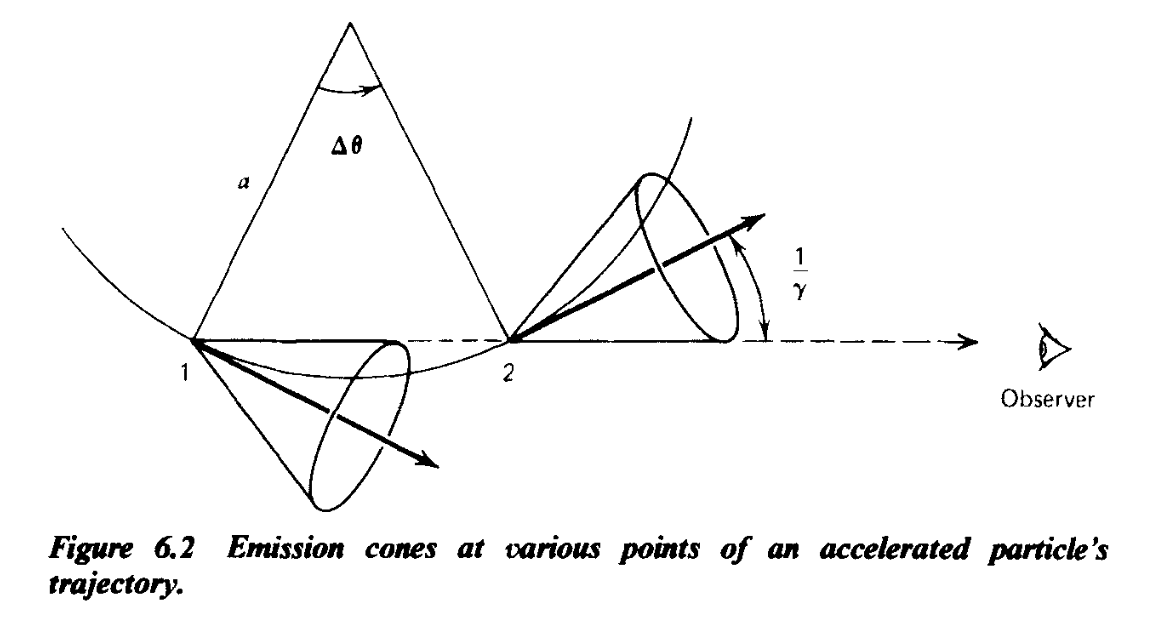
\includegraphics[width=0.75\linewidth]{Pictures/figures/rybicki_lightman_6_2.png}
    \caption{Emission cones at various points of an accelerated particle's trajectory. Taken from Rybicki \& Lightman}
    \label{fig:synchrotron_emission_cone}
\end{figure}

By looking at figure~\ref{fig:synchrotron_emission_cone}, we can see that $\Delta \theta \sim 2/\gamma \implies \Delta s = 2a/\gamma$. Likewise, the radius of the helix is given by
\[
r = \frac{v}{\omega_B \sin \varphi},
\]
where $\varphi$ is the angle between the field and the velocity (the pitch angle). Now, the beginning of the pulse occurs when the cone first passes us at $t=0$ and ends $\Delta s$ along the path later when the observer leaves the cone. This is
\[
\Delta t = \frac{2v}{\gamma \omega_B \sin \varphi}
\]
Now, the traveled distance is different by, again, $\Delta s/c$ because one edge of the beam is emitted closer and on further. Thus,
\[
\Delta t_{\rm observed} = \frac{2}{\gamma \omega_B \sin \varphi}(1-\beta).
\]
Noting that $1-\beta \approx 1/2\gamma^2$, we have
\[
\Delta t \sim \frac{1}{\gamma^3 \omega_B \sin \varphi}.
\]
This therefore defines a \textbf{critical frequency cutoff at $1/\Delta t$}. We therefore define the \textbf{synchrotron cutoff frequency} as 
\[
\omega_c = \frac{3}{2} \gamma^3 \omega_B \sin \varphi.
\]
\par
It turns out that the \textbf{electric field depends on $\theta$ only by $\gamma \theta$}, which is a manifestation of the relativistic beaming we have been talking about. \rmk{See 4.8 of Rybicki-Lightman for a detailed explaination of this assertion.} We can therefore say that
\[
E(t) \sim F(\gamma \theta(t)).
\]
It can be shown by arguments similar to those above that $\gamma \theta \propto \omega_c t$, so $E(t) \propto g(\omega_c t)$. \rmk{We're being fairly phenomenological; however, we can say at this stage that we have some constant (independent of $t$) in front of this unknown spectral function $g(\omega_c t)$. This is still enough for us to start investigating the Fourier modes.} If we expand in Fourier space,
\[
\hat{E}(\omega) \propto \int_{-\infty}^\infty g(\omega_ct) e^{i\omega t} dt = \int_{-\infty}^{\infty} g(\xi) \exp(i\omega\xi/\omega_c)\;d\xi.
\]
Now, $dW/dt d\Omega$ is proportional to the square of the fourier modes, so if we integrate over the solid angles and divide by the orbital period to get rid of any remaining time dependence, we have
\[
\frac{dW}{dt d\omega} = C_1F\left(\frac{\omega}{\omega_c}\right).
\]
By comparing this constant to the Larmour formula above, we find
\[
\boxed{
P(\omega) = \frac{\sqrt{3}}{2\pi} \frac{q^3B\sin\varphi}{mc^2} F\left(\frac{\omega}{\omega_c}\right).
}
\]
\subsection{Effective Power Laws}

Let's consider a region of frequency where $P(\omega) \propto \omega^{-k}$. It is often the case that relativistic electrons have statistical distributions which are also power-law like in the sense that
\[
N(E) dE \sim CE^{-p}\; dE
\]
over some energy band. If we therefore integrate the single particle radiation behavior over all particles at various energies, then
\[
P_{\rm tot}(\omega) \sim C\int_{\gamma_1}^{\gamma_2} P(\omega) \gamma^{-p} d\gamma \propto \int_{\gamma_1}^{\gamma_2} F\left(\frac{\omega}{\omega_c}\right) \gamma^{-p}\;d\gamma.
\]
under a change of variables $x \propto \omega/\gamma^2$, we have
\[
P_{\rm tot} \propto \omega^{-(p-1)/2} \int_{x_1}^{x_2} F(x)x^{(p-3)/2} \;dx
\]
so we conclude the very important statement that the \textbf{power law behavior of the electrons is linked to the power law of the spectrum:}
\[
k = \frac{p-1}{2}.
\]

\section{The High Energy Picture}

We have now discussed a number of highly relevant sources of emission in high energy astrophysics and we now wish to place them into perspective somewhat. we'll go through band by band and look at the relevant processes.

\subsection{Soft X-ray Emission ($E \lesssim 10\;\mathrm{keV}$)}

The soft X-ray band encompasses photon energies below about $10\;\mathrm{keV}$,
corresponding to thermal equivalents $T \lesssim 10^8\;\mathrm{K}$.
Several distinct processes can contribute in this regime:

\begin{itemize}
    \item \textbf{Blackbody emission from hot, optically thick sources.}
    For objects with surface temperatures $\gtrsim 10^6$--$10^7\;\mathrm{K}$,
    such as neutron stars or the innermost regions of accretion disks,
    thermalized radiation can extend into the soft X-ray band. The
    requirement of high temperature and optical thickness means that
    such spectra are comparatively rare.

    \item \textbf{Thermal bremsstrahlung from hot, diffuse plasmas.}
    This is the dominant emission mechanism in galaxy clusters and
    supernova remnants, where intracluster gas reaches
    $T \sim 10^7$--$10^8\;\mathrm{K}$. Because the gas is optically
    thin, photons escape directly without thermalization, producing a
    continuum spectrum characteristic of free--free emission rather than
    a blackbody.

    \item \textbf{Line emission from heavy ions.}
    Soft X-ray spectra often show rich line features from
    highly ionized elements (e.g.~Fe, O, Ne, Mg). The strength of these
    lines depends sensitively on the plasma temperature:
    \begin{itemize}
        \item At lower soft X-ray temperatures ($T \sim 10^6\;\mathrm{K}$),
              lighter elements (C, N, O) dominate.
        \item At higher temperatures ($T \gtrsim 10^7\;\mathrm{K}$),
              heavier ions (Si, S, Fe) contribute strong line complexes.
    \end{itemize}
    These lines provide powerful diagnostics of plasma temperature,
    density, and chemical composition.
\end{itemize}

\begin{remark}
    \textbf{Summary:} In the soft X-ray band, the most common emission
    mechanisms are thermal in nature: blackbody emission from very hot
    optically thick surfaces, free--free emission from hot optically
    thin plasmas, and line emission from highly ionized heavy elements.
    The relative importance of these components provides a direct probe
    of the physical state of the emitting plasma.
\end{remark}

\subsection{Hard X-ray Emission ($\sim 10$--$100\;\mathrm{keV}$)}

In the hard X-ray band, the character of emission changes
substantially compared to the soft X-ray regime. The key point is that
\textbf{thermal processes become inefficient}:

\begin{itemize}
    \item \textbf{Blackbody emission fails.}  
    To produce significant flux at $E \gtrsim 10\;\mathrm{keV}$, a
    blackbody would require temperatures $T \gtrsim 10^9\;\mathrm{K}$,
    which are rarely realized in optically thick astrophysical objects.
    As a result, blackbody radiation does not extend naturally into the
    hard band.

    \item \textbf{Thermal bremsstrahlung cutoff.}  
    The exponential factor $\exp(-h\nu/kT)$ in the free--free spectrum
    rapidly suppresses emission once $h\nu \gg kT$. Unless the plasma
    temperature exceeds $T \sim 10^8\;\mathrm{K}$, bremsstrahlung
    produces little flux in the hard band. Thus, galaxy clusters and
    supernova remnants, while bright in soft X-rays, are strongly
    suppressed here.

    \item \textbf{Emergence of non--thermal processes.}  
    In this band the dominant mechanisms are non--thermal:
    \begin{enumerate}
        \item \emph{Inverse Compton scattering (Comptonization):}
              seed photons (e.g.~UV or soft X-rays from accretion disks)
              are upscattered by hot or relativistic electrons in
              coronae, producing hard power--law tails.
        \item \emph{Non--thermal bremsstrahlung:} accelerated electrons
              colliding with ambient ions can yield a hard continuum.
    \end{enumerate}
    These processes naturally give rise to \textbf{power--law spectra}
    rather than exponential cutoffs, a hallmark of the hard X-ray band.
\end{itemize}

\begin{remark}
    \textbf{Summary:} The hard X-ray regime marks the transition from
    thermal to non--thermal astrophysics. Blackbody and thermal
    bremsstrahlung contributions are exponentially suppressed, while
    non--thermal processes such as inverse Compton scattering and
    non--thermal bremsstrahlung dominate the emission.
\end{remark}

\subsection{Low-Energy Gamma Rays ($10\;\mathrm{keV}$--$10\;\mathrm{MeV}$)}

Moving into the low-energy gamma-ray regime, additional processes
become important:

\begin{itemize}
    \item \textbf{Isomeric nuclear transitions.}  
    In addition to electron excitations, nuclei themselves can occupy
    \emph{metastable excited states}, called \emph{nuclear isomers}. Much
    like electronic fluorescence, these states may decay back to the nuclear
    ground state via the emission of a photon, but here the photon energy is
    set by nuclear rather than electronic binding energies. As a result, the
    transitions occur in the $\sim 100\;\mathrm{keV}$ to $\sim \mathrm{MeV}$
    range, producing \textbf{narrow gamma-ray lines}. These nuclear
    de-excitations are distinct from beta decay: no change in proton or
    neutron number occurs, only a rearrangement of nucleons within the same
    nucleus. 
    
    In contrast, \textbf{beta decay} involves the weak interaction and a
    transmutation of the nucleus (neutron $\to$ proton or vice versa). Many
    beta decays do leave the daughter nucleus in an excited state, which
    then de-excites by emitting gamma rays at characteristic energies. Thus
    gamma-ray lines can arise either from \emph{direct isomeric transitions}
    or from \emph{secondary de-excitations following beta decay}. In both
    cases, the resulting line features provide direct probes of
    nucleosynthesis and the isotopic composition of astrophysical sources
    (e.g.~supernova ejecta, radioactive isotopes in the interstellar medium).

    \item \textbf{Electron--positron annihilation.}  
    Pair annihilation produces the characteristic $511\;\mathrm{keV}$
    line, often accompanied by a continuum from in--flight annihilation
    or positronium formation. This process is relevant in compact object
    environments where pair plasmas can form.
\end{itemize}

\begin{remark}
    \textbf{Summary:} At low gamma-ray energies, line processes emerge
    alongside continua. Nuclear transitions yield discrete spectral
    features, while pair annihilation produces the distinct 511 keV
    line, a key diagnostic of relativistic pair plasmas.
\end{remark}

\subsection{Medium Energy Gamma Rays ($140\;\mathrm{MeV}$--$10\;\mathrm{GeV}$)}

In this band, new processes appear that are rooted in hadronic
interactions rather than atomic or nuclear transitions.

\begin{itemize}
    \item \textbf{Pion production and decay.}  
    The neutral pion has a rest mass of $m_{\pi^0} c^2 \simeq
    135\;\mathrm{MeV}$. In high--energy environments, collisions of
    relativistic protons or heavier nuclei (``cosmic rays'') with
    ambient matter can produce pions. The neutral pion rapidly decays
    via
    \[
        \pi^0 \;\to\; \gamma + \gamma,
    \]
    yielding two photons each with energies of order
    $\sim 70\;\mathrm{MeV}$ in the pion rest frame. In astrophysical
    sources, boosted pions produce broad $\gamma$--ray spectra peaking
    in the $\sim 100\;\mathrm{MeV}$--GeV range.

    \item \textbf{Charged pion channels.}  
    Charged pions ($\pi^\pm$) decay into muons and neutrinos, and the
    resulting leptons can further radiate (via synchrotron or inverse
    Compton) and contribute continuum emission in this band.

    \item \textbf{Astrophysical relevance.}  
    Medium--energy $\gamma$ rays are a \emph{smoking gun} for hadronic
    processes: detecting the characteristic ``pion bump'' around
    100--200 MeV provides direct evidence of cosmic ray protons
    colliding with ambient matter. This is a key diagnostic in supernova
    remnants, molecular clouds, and active galactic nuclei where cosmic
    ray acceleration is expected.
\end{itemize}

\begin{remark}
    \textbf{Summary:} The $140\;\mathrm{MeV}$--$10\;\mathrm{GeV}$ band
    is dominated by \emph{pion production and decay}. Neutral pions
    decay directly to gamma rays, producing a distinctive spectral
    feature, while charged pions generate leptons and neutrinos that
    feed into broader non--thermal emission channels. Observations in
    this band directly probe the hadronic component of cosmic rays.
\end{remark}


\subsection{High Energy Gamma Rays ($>10\;\mathrm{GeV}$)}

In the very high energy $\gamma$--ray regime, emission is purely
non--thermal. The dominant processes involve relativistic particle
populations interacting with background fields:

\begin{itemize}
    \item \textbf{Inverse Compton scattering.}  
    Relativistic electrons with Lorentz factor $\gamma$ can upscatter
    background photons of energy $E$ to
    \[
        E_{\rm sc} \;\sim\; \gamma^2 E,
    \]
    provided the scattering occurs in the Thomson limit
    ($E' \ll m_e c^2$ in the electron rest frame).
    For example:
    \begin{itemize}
        \item CMB photons ($E \sim 10^{-3}\,\mathrm{eV}$) scattered by
              $\gamma \sim 10^6$ electrons produce
              $E_{\rm sc} \sim 1\;\mathrm{GeV}$--TeV photons, still
              within the Thomson regime because
              $\gamma E \sim 1\;\mathrm{keV} \ll m_e c^2$.
        \item Optical/UV photons ($E \sim 1\;\mathrm{eV}$) with the same
              $\gamma \sim 10^6$ electrons would yield
              $E_{\rm sc} \sim 1\;\mathrm{TeV}$, but now
              $\gamma E \sim 1\;\mathrm{MeV} \gtrsim m_e c^2$,
              pushing the interaction into the
              \textbf{Klein--Nishina regime}, where the cross section is
              suppressed and the maximum scattered photon energy is
              limited to $\sim \gamma m_e c^2 \approx 500\;\mathrm{GeV}$.
    \end{itemize}
    Thus, inverse Compton scattering can remain efficient into the VHE
    band, but only if the seed photons are sufficiently low in energy
    (CMB, IR). For optical/UV seed fields, KN suppression becomes
    significant.

    \item \textbf{Hadronic pion decay.}  
    Relativistic protons colliding with gas produce $\pi^0$ mesons,
    which decay into $\gamma$--rays. This channel remains efficient at
    $>10\;\mathrm{GeV}$ and is often invoked to explain spectra from
    supernova remnants, AGN jets, and cosmic ray interactions in the
    interstellar medium.

    \item \textbf{Synchrotron and curvature radiation.}  
    Extremely energetic electrons in strong magnetic fields can radiate
    into the GeV--TeV range. This is important in pulsar wind nebulae,
    magnetars, and compact object magnetospheres.
\end{itemize}

\begin{remark}
    \textbf{Summary:} Above $\sim 10\;\mathrm{GeV}$, all emission is
    non--thermal. Inverse Compton scattering is efficient for low-energy
    seed photons (CMB, IR) but enters the Klein--Nishina regime for
    optical/UV/X-ray fields, reducing efficiency and altering spectral
    shapes. Hadronic pion decay and extreme synchrotron/curvature
    emission provide additional channels, making this band a key probe
    of both relativistic leptons and hadrons in astrophysical sources.
\end{remark}


\chapter{Detection of High Energy Photons}
There are generically \textbf{3 ways} that high energy photons interact with matter and lose energy:
\begin{enumerate}
    \item photoelectric absorption
    \item pair production
    \item Compton scattering
\end{enumerate}
Of these, both \textbf{photoelectric absorption} and \textbf{pair production} can be used as methods of detecting high energy photons.
\begin{remark}
    We also can use low energy photons to study high energy processes, for example the synchrotron radiation of a highly relativistic source will often be, nonetheless, broad enough that radio telescopes can be used.
\end{remark}

\section{Photoelectric Absorption}

In some scenarios, an incident photon of energy $E = h\nu$ has
sufficient energy to remove an electron from an atom, resulting in
\textbf{photoionization}. The resulting electron energy will be
\[
    E_{e^-} = h\nu - E_{\rm binding}.
\]
Electrons may be ejected from any of the bound shells of an atom (K, L,
M, N, etc.), depending on whether the photon energy exceeds the
corresponding binding energy. These binding energies differ
substantially:
\begin{itemize}
    \item The innermost K--shell electrons are bound most tightly,
          typically with energies in the keV range for medium and
          heavy elements.
    \item Outer--shell (L, M, N) electrons have progressively lower
          binding energies, often in the eV to hundreds of eV range.
    \item As $h\nu$ increases past each threshold, new ionization
          channels open up, leading to discontinuities in the
          cross section called \textbf{absorption edges}.
\end{itemize}
These level--dependent thresholds are astrophysically and
experimentally important. In astrophysics, they imprint strong edges
and absorption features in X--ray spectra. In detector physics, they
set the energy ranges where a material efficiently absorbs photons:
materials with K--shell binding energies in the keV range (e.g.~Si,
Ge, or heavier metals) are ideal for building X--ray detectors.

\subsection{The Photoelectric Cross Section}

\begin{figure}[th!]
    \centering
    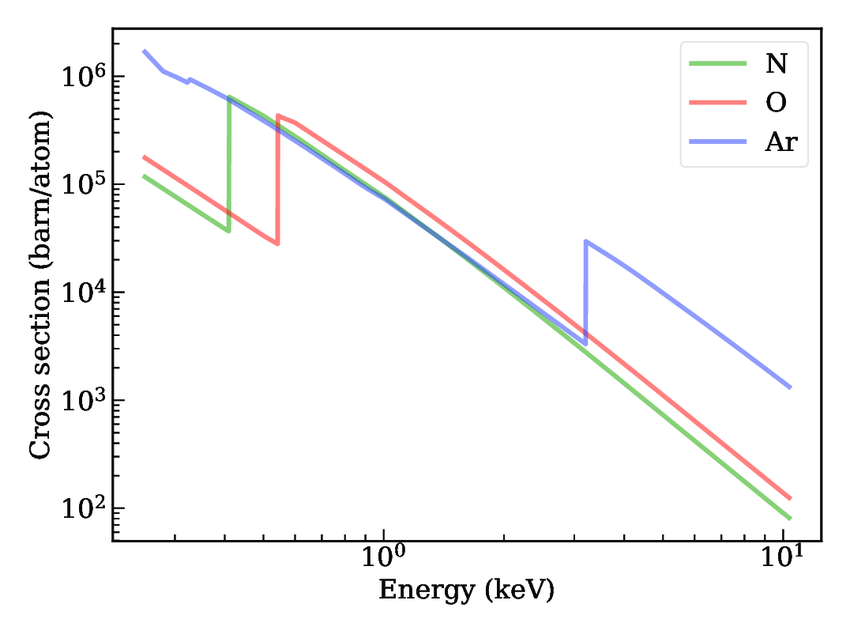
\includegraphics[width=0.75\linewidth]{Pictures/figures/photo_ion_cross_section.png}
    \caption{K-edges for various elements.}
    \label{fig:k_edges_photo_ionization}
\end{figure}

\begin{figure}
    \centering
    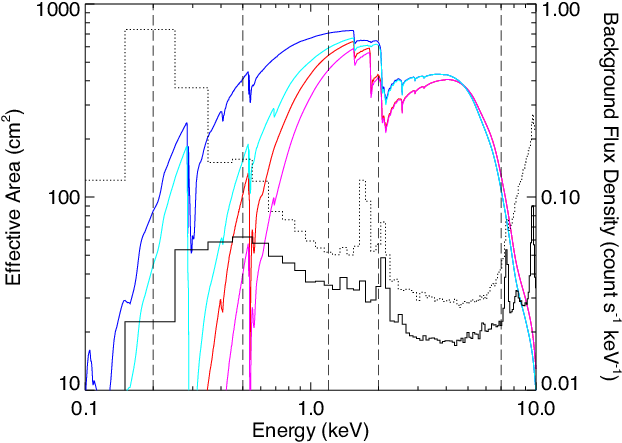
\includegraphics[width=0.75\linewidth]{Pictures//figures/chandra_effective_area.png}
    \caption{The effective area of chandra, featuring distinctive edges corresponding to the K-edges of the detector.}
    \label{fig:chandra_effective_area}
\end{figure}

For $h\nu \gg E_{\rm binding}$ but $h\nu \ll m_e c^2$, we are in a
semi--classical regime and the photoionization cross section scales as
\[
    \sigma_{\rm pi} \;\sim\; Z^5 (h\nu)^{-7/2}.
\]

\paragraph{Intuition for the scaling.}
This dependence can be understood from two complementary points of view:

\begin{itemize}
    \item \emph{$Z^5$ dependence.}  
    The hydrogenic wavefunction for an inner electron scales roughly as
    $\psi_{1s}(0) \sim Z^{3/2}$ near the nucleus. Since the transition
    probability involves the square of the matrix element, the overlap
    with the continuum grows rapidly with $Z$, leading to an overall
    scaling $\propto Z^5$ once phase--space and dipole factors are
    included. Heavier atoms therefore have much larger photoelectric
    cross sections.
    
    \item \emph{$(h\nu)^{-7/2}$ dependence.}  
    At high photon energies, the outgoing electron carries momentum
    $p \sim \sqrt{2 m_e h\nu}$ and its wavefunction oscillates rapidly.
    The overlap with the compact bound--state wavefunction is therefore
    strongly suppressed at large $p$. Quantitatively, the dipole matrix
    element falls off like $p^{-3}$ while the continuum density of
    states contributes a factor $\sim p$. Together these give a net
    $\nu^{-7/2}$ scaling of the cross section.
\end{itemize}

\begin{remark}
    \textbf{Key Points:}
    \begin{enumerate}
        \item Larger $Z$ $\;\Rightarrow\;$ much higher cross section,
              since inner--shell electrons are more tightly bound and
              concentrated near the nucleus.
        \item Larger $h\nu$ $\;\Rightarrow\;$ much lower cross section,
              since fast photoelectrons overlap poorly with the bound
              state wavefunction.
        \item This explains the characteristic behavior: large jumps at
              each absorption edge, followed by a steep decline as
              $\nu^{-7/2}$ until the next edge.
    \end{enumerate}
\end{remark}

\section{Pair-Production}

At energies higher than a few keV, the cross section for \textbf{photo-ionization drops off sharply} and we are no longer able to use the same methodologies for detectors. We therefore rely on an alternative which emerges for sufficiently high energy photons: \textbf{pair production}. There are 2 relevant mechanisms:
\begin{enumerate}
    \item \textbf{Nuclear Pair Production} $(\gamma \to e^{-} + e^{+})$ is only possible in an electro-magnetic field in order to conserve momentum and energy.
    \item \textbf{Annihilation} $(\gamma + \gamma \to e^{-} + e^{+})$.
\end{enumerate}

\subsection{Nuclear Pair Production}

Formally, $\gamma \to e^{-} + e^{+}$ cannot conserve both momentum and energy at the same time. This problem stems from the fact that the produced electrons must travel parallel to the original photon because momentum must be conserved. Working out the math, one finds that such a pair \textbf{can happen in close proximity to a nucleus}. The cross section follows the general scaling
\[
\sigma_{\rm pair} \sim \underbrace{\alpha}_{\text{fine-structure}} \sigma_T Z^2 f(\nu).
\]
\par
Another relevant feature of this emission is that we require 
\[
h \nu \ge 2 E_{\rm electron} = 2m_e c^2 \approx 1 \rm {MeV}.
\]

\subsection{Annihilation}
Famously, the inverse of the pair production process is annihilation, which produces two photons at 511 keV. We have clear evidence in our own galaxy for this process occurring.

\subsubsection{Angular Dependence}
Two photons of energies $h\nu_1$ and $h\nu_2$ colliding at angle
$\theta$ can annihilate to produce an $e^+e^-$ pair, provided there is
sufficient center--of--mass (COM) energy. The threshold condition comes
from requiring the invariant squared COM energy $s$ to exceed
$4m_e^2c^4$:
\[
    s = 2 h\nu_1 h\nu_2 (1 - \cos\theta) \;\;\geq\;\; (2m_e c^2)^2.
\]
Equivalently,
\[
    h\nu_1 h\nu_2 \;\geq\;
    \frac{(m_e c^2)^2}{1 - \cos\theta}.
\]

\paragraph{Angular dependence.}
\begin{itemize}
    \item For head--on collisions ($\theta = \pi$), the threshold is
          minimal: $h\nu_1 h\nu_2 \geq (m_e c^2)^2$.
    \item For smaller angles, the denominator decreases, raising the
          required photon energies; nearly parallel photons require
          unrealistically high energies.
\end{itemize}

\paragraph{Cross section.}
The full QED calculation gives a cross section
$\sigma_{\gamma\gamma\rightarrow e^+e^-}$ that:
\begin{enumerate}
    \item vanishes at threshold,
    \item rises rapidly just above threshold to a maximum of order
          $\sim 0.2\,\sigma_T$ (where $\sigma_T$ is the Thomson cross
          section),
    \item falls off gradually at higher energies.
\end{enumerate}
The dependence on $(1-\cos\theta)$ means that interactions are
dominated by head--on collisions.

\begin{remark}
    \textbf{Key Points:}
    \begin{enumerate}
        \item Pair production requires sufficient COM energy, expressed
              by the invariant threshold condition.
        \item The process is strongly angle dependent, favoring head--on
              photon collisions.
        \item The cross section peaks just above threshold and is always
              $\lesssim \sigma_T$.
    \end{enumerate}
\end{remark}

\section{The Combined Picture}

Having discussed the two major mechanisms for high energy photon detection, we can see that the desired bandpass of the instrument largely dictates the method of detection.

\begin{figure}[h!]
    \centering
    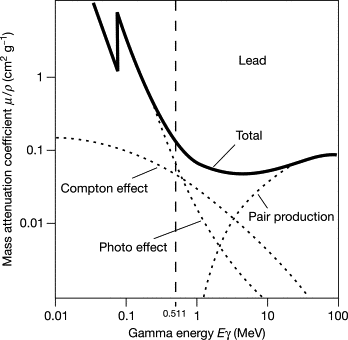
\includegraphics[width=0.75\linewidth]{Pictures//figures/gamma_cross_section.png}
    \caption{The combined cross sections for different absorption mechanisms of high energy photons.}
    \label{fig:high_energy_absorption_cross_section}
\end{figure}

\part{Accretion Physics}
\chapter{Introduction to Accretion}
It has been known for a long time that gravitational energy is insufficient to completely power the sun for its lifetime; however, in recent decades, it has become apparent that there are other contexts in which gravitation is the \textbf{sole adequate engine} for a number of different phenomena. This includes AGN and quasars, TDEs, and a number of other observed systems featuring compact objects.
\par
In a general sense, we might consider a system containing a compact object of mass $M$ and radius $R$. If a mass $m$ falls from $\infty$ into the surface of the compact object, it will gain
\[
K = \frac{GMm}{R}
\]
in kinetic energy.
\vspace{0.25cm}
\begin{itemize}
    \item For \textbf{stellar objects}, the kinetic energy per unit mass extracted from this process is
    \[
    \epsilon = 2 \times 10^{15}\left(\frac{M}{M_\odot}\right)\left(\frac{R}{R_\odot}\right)^{-1} \;{\rm erg\;s^{-1}}.
    \]
    \item For \textbf{compact objects}, where $GM/R \sim c^2$, one finds instead that
    \[
    \epsilon \approx 9\times 10^{20}\;{\rm erg\;s^{-1}}.
    \]
\end{itemize}
\vspace{0.25cm}
For reference, a nuclear reaction with efficiency $\eta$ would yield
\[
\epsilon \approx \eta c^2, \;\text{for typical $\eta \sim 10^{-3}$,}\; \epsilon \approx 10^{18}\;{\rm erg\; s^{-1}}.
\]
Thus, we see that while \textbf{gravitational energy is subdominant for stellar objects}, it can be \textbf{highly energetic for compact objects}.
\par

\begin{bigidea}
    The study of accretion is the study of two effects:
\begin{enumerate}
    \item The \textbf{flow of material to the surface of the accretor}, which is a largely well understood problem, and
    \item The \textbf{radiation of energy / distribution of angular momentum}, which remains a very active field of research in astrophysics to this day.
\end{enumerate}
\end{bigidea}

\section{The Eddington Limit}

In this section, we introduce the \textbf{Eddington accretion limit}, which is an effective metric for the limitation of "normal" accretion.
\par
Consider an accretion scenario in which \textbf{fully ionized Hydrogen} accretes onto a central body. If that central body has a bolometric luminosity $L_{\rm bol}$, then the incident photons will exert a \textbf{radiation pressure} on the in-falling material. The energy transport per unit area at distance $r$ from the surface is
\[
|{\bf S}| = \frac{L_{\rm bol}}{4\pi r^2} \implies P_{\rm rad} = \frac{L_{\rm bol}}{4\pi r^2 c}.
\]
The dominant interaction mechanism with be \textbf{Thompson scattering off free electrons}, and so the Thompson cross section determines the relevant force on the particles:
\[
F = \frac{L_{\rm bol}\sigma_T}{4\pi r^2 c}.
\]
\rmk{There are actually two statements here that get swept under the rug. First off, we assume Thompson scattering is dominant over other forms of interaction. This is fine \textit{if} we don't have magnetic fields or very high temperature gas. As long as we are below $\sim 100\;{\rm keV},$ we're still in the non-relativistic regime of Thompson and don't have to treat Compton. We also recognize that $\sigma_{\rm thompson} \sim r_0^2 \sim m^{-2}$, so the electrons are the dominant source of scatter, not the protons. Because they are tightly coupled, both will effectively get dragged along.}
\par
Now, the gravitational force per electron-proton pair is
\[
F_{\rm grav} = - \frac{GM(m_p+m_e)}{r^2} \approx - \frac{GMm_p}{r^2},
\]
so
\[
F \le 0 \implies \frac{GMm_p}{r^2} \ge \frac{L_{\rm bol} \sigma_T}{4\pi r^2 c} \implies L_{\rm bol} = 4\pi G M m_p c / \sigma_T.
\]
This leads us to the formal definition of the \textbf{Eddington Luminosity}:
\vspace{0.5cm}
\begin{definition}[Eddington Luminosity]
The \textbf{Eddington Luminosity} is defined to be
\begin{equation}
    \label{eq:eddington_luminosity}
    \boxed{
    L_{\rm Edd} = \frac{4\pi GMm_p c}{\sigma_T} = 1.3 \times 10^{38} \; \left(\frac{M}{M_\odot}\right) \;\rm{ergs\;s^{-1}}.
    }
\end{equation}
It is the \textbf{maximum luminosity at which accretion can occur}.
\end{definition}


\subsection{Super-Eddington Sources}
The derivation of the Eddington luminosity implicitly assumes several caveats:
\vspace{0.25cm}
\begin{enumerate}
    \item \textbf{Interaction mechanism:} We assume that the dominant coupling between photons and matter is \emph{Thomson scattering} off free electrons. This is valid as long as the characteristic photon energies are $\lesssim 100 \,{\rm keV}$, so that Klein--Nishina (Compton) corrections are negligible, and no strong magnetic fields introduce cyclotron or resonant scattering processes.
    \item \textbf{Scatterers:} Because $\sigma_T \propto m^{-2}$, electrons dominate the scattering cross section compared to protons. Electrons and protons are coupled via Coulomb forces, so the radiation effectively drags along the entire electron--proton plasma.
    \item \textbf{Opacity:} We treat the opacity as a pure scattering opacity given by $\kappa = \sigma_T/m_p$. In realistic astrophysical systems, bound-free absorption, free-free opacity, or dust scattering may be important and can modify the effective Eddington limit.
    \item \textbf{Geometry and symmetry:} The calculation assumes spherical symmetry and isotropic radiation. In accretion disks, anisotropic emission and beaming effects can allow accretion to exceed the nominal Eddington luminosity locally.
    \item \textbf{Steady-state assumption:} The Eddington limit describes a balance between radiation pressure and gravity in an ideal steady-state system. Transient or time-dependent accretion flows may temporarily surpass $L_{\rm Edd}$.
\end{enumerate}
\vspace{0.25cm}
Thus, while $L_{\rm Edd}$ provides a robust benchmark for the ``normal'' luminosity limit of accreting systems, real astrophysical environments can deviate from this simple picture. There are many examples of such systems:
\vspace{0.25cm}
\begin{itemize}
    \item \textbf{Ultraluminous X-ray sources (ULXs):} Compact objects in external galaxies with apparent luminosities $\gtrsim 10^{39}\,\mathrm{erg\,s^{-1}}$, above the Eddington limit for a stellar-mass black hole. These are thought to involve either beaming effects or accretion onto neutron stars with strong magnetic fields.
    \item \textbf{Tidal disruption events (TDEs):} When a star is torn apart by a supermassive black hole, the fallback of stellar debris can briefly power emission well above the Eddington luminosity.
    \item \textbf{Supermassive black hole growth (quasars):} Some quasars, especially in the early universe, show evidence for sustained super-Eddington accretion, which may explain how black holes grew rapidly to billions of solar masses within a few hundred million years.
\end{itemize}
\vspace{0.25cm}
In short, while the Eddington luminosity provides a useful benchmark, nature finds several ways to circumvent it, making super-Eddington accretion a key ingredient in high-energy astrophysics.

\section{Characterizing Accretion Emission}

\subsection{The Accretion Luminosity}
The fact that there is a natural scale for viable accretion powered luminosity, it becomes worth asking the question: \textbf{how much luminosity do we get from accretion?} In general, this is a complex question and not easily constrained; however, we might make a broad characterization by defining the \textbf{accretion luminosity}, which is the \textit{total released energy assuming perfect conversion}:
\begin{equation}
    \label{eq:accretion_luminosity}
    \boxed{
    L_{\rm acc} = \frac{GM\dot{M}}{R} = \begin{cases}
        1.3 \times 10^{33} \;\dot{M}_{16} \left(\frac{M}{M_\odot}\right) \left(\frac{10^9\;{\rm cm}}{R}\right)\;{\rm ergs\;s^{-1}},&\text{W.D.}\\
        1.3 \times 10^{36}  \;\dot{M}_{16} \left(\frac{M}{M_\odot}\right) \left(\frac{10^6\;{\rm cm}}{R}\right)\;{\rm ergs\;s^{-1}},&\text{N.S.}
    \end{cases}
    }
\end{equation}
where $\dot{M} = 10^{16}\;\dot{M}_{16} \;{\rm g\;s^{-1}}.$ \rmk{For accretion onto binary systems, $\dot{M}_{16}\sim 1$ for most systems, justifying its introduction.} 
\begin{remark}
    We \textbf{formally} acknowledge that $L_{\rm acc} \neq L_{\rm Obs}$ in most relevant scenarios. $L_{\rm acc}$ is not really the \textbf{observed luminosity}, but instead the upper bound on the luminosity. 
\end{remark}
\par
The above equation relies on our ability to specify a relevant $R$; however, we might actually have energy released at lower radii or inefficient energy release. We therefore introduce a \textbf{alternative definition}
\begin{equation}
    L_{\rm acc} = \eta c^2 \dot{M},
\end{equation}
where $\eta$ is the \textbf{accretion efficiency}. 
\begin{remark}
    $\eta$ is a \textbf{tricky parameter} because the theorist will draw a distinction between $\eta = L_{\rm acc}/(\eta \dot{M})$ while the observer will say that $\eta = L_{\rm Obs}/(\eta \dot{M})$. We may also apply this definition for \textbf{non-compact objects with definite radius}: $\eta$ swallows up the weird dependencies on $G$ and $R$.
\end{remark}
Based on this, we can let $L_{\rm acc} = L_{\rm Edd}$ and therefore derived the very important \textbf{Eddington Accretion Rate (EAR)}
\begin{equation}
\boxed{
    \dot{M}_{\rm Edd} = \frac{L_{\rm Edd}}{\eta c^2} = \frac{4\pi G M m_p}{\sigma_T \eta c}}
\end{equation}
The relevant scaling goes as
\[
 \dot{M}_{\rm Edd} = \eta^{-1}\; 1.4 \times 10^{17}\; \left(\frac{M}{M_\odot}\right)\;{\rm g\; s^{-1}} = \eta^{-1}\;2.2 \times 10^{-9} \left(\frac{M}{M_\odot}\right)\; {\rm M_\odot\;yr^{-1}}.
\]


\subsection{The Emitted Spectrum}

An important question in accretion physics is: \textbf{what spectrum of radiation is produced by the accretion flow?}  The answer depends on how efficiently the liberated gravitational energy thermalizes and how photons interact with the surrounding medium.  Several characteristic temperatures are useful for bounding the expected emission. The first of which is the estimated, intrinsic temperature of the emitted photons:
\vspace{0.5cm}
\begin{definition}[Radiation Temperature]
\label{def:rad_temperature}
The \textbf{radiation temperature} $T_{\rm rad}$ is the effective temperature of the emergent photons,
\begin{equation}
    \label{eq:rad_temp}
    T_{\rm rad} = \frac{h\left<\nu\right>}{k_b} = 1.16\times 10^{7} \left(\frac{h\bar{\nu}}{1\;{\rm keV}}\right)\;{\rm K}.
\end{equation}
\end{definition}
\vspace{0.5cm}

Now, depending on the nature of the source, $T_{\rm rad}$ may range considerably. There are a number of other proxies which are used and which provide useful order-of-magnitude bounds for $T_{\rm rad}$.
\vspace{0.25cm}
\begin{definition}[Thermal Temperature]
\label{def:thermal_temperature}
The \textbf{thermal temperature} $T_{\rm thermal}$ is the temperature obtained if the full gravitational potential energy released by accretion were converted into thermal energy of the gas. Formally, for a monatomic gas, 
\begin{equation}
    \label{eq:thermal_temperature}
    T_{\rm thermal} = \frac{GMm_p}{3k_bR}= \frac{2U_{\rm grav, proton}}{k_b}. 
\end{equation}
It provides an \emph{upper bound} on heating. In principle, if accretion is highly efficient and optically thin, we expect emission to have a characteristic temperature similar to $T_{\rm thermal}$.
\end{definition}
\vspace{0.25cm}
\begin{definition}[Virial Temperature]
\label{def:virial_temperature}
The \textbf{virial temperature} $T_{\rm virial}$ characterizes gas in virial equilibrium, where the thermal energy is about half of the gravitational potential energy. 
Thus, $T_{\rm virial} \simeq \tfrac{1}{2}T_{\rm thermal}$, making it a more realistic estimate for the gas near the accretor.
\end{definition}
\vspace{0.25cm}
\begin{definition}[Brightness Temperature]
\label{def:brightness_temperature}
The \textbf{brightness temperature} $T_b$ is the blackbody temperature a source would need to radiate the observed flux. 
\begin{equation}
    \label{eq:brightness_temperature}
    T_b = \left(\frac{L_{\rm acc}}{4\pi R^2 \sigma_{\rm sb}}\right)^{1/4}.
\end{equation}
It serves as the observable counterpart to $T_{\rm rad}$ in the optically thick case and is generally a a good lower bound on $T_{\rm rad}$.
\end{definition}
\vspace{0.5cm}

\begin{bigidea}
    The emitted spectrum of an accretion flow is bounded by these characteristic scales:  
    \[
    T_{\rm virial} \;\;\lesssim\;\; T_{\rm rad},\,T_b \;\;\lesssim\;\; T_{\rm thermal}.
    \]  
    \textbf{Takeaway:} The precise emission depends on opacity and optical depth, but these temperatures provide natural limits on what can be observed.
\end{bigidea}

\section{Accreting Systems and Their Properties}
\begin{figure}[ht!]
    \centering
    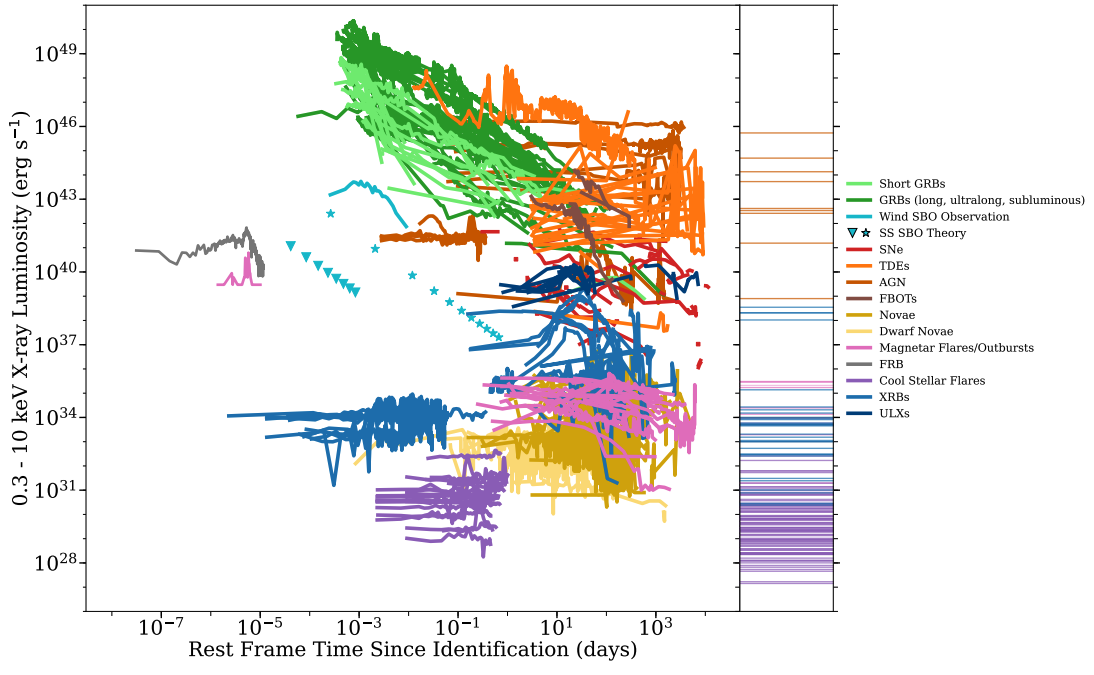
\includegraphics[width=\linewidth]{Pictures/figures/xray_sources.png}
    \caption{X-ray phase space of transients and variable phenomena, including gamma-ray burst (GRB) afterglows, supernovae (SNe), supernova shock breakouts (SBOs), tidal disruption events (TDEs) and active galactic nuclei (AGN), fast blue optical transients (FBOTs), cataclysmic variables, magnetar flares/outbursts and fast radio bursts, cool stellar flares, X-ray binary outbursts, and ultraluminous X-ray sources. Main Panel: X-ray luminosity evolution with rest-frame time since identification. Theoretical SBO peak Lx-duration points are shown with different symbols corresponding to the model’s input parameters; see Section 2.2 for details. Right Side Panel: To offer a sense of their persistent behavior, the quiescent/pre-flare luminosities of the included variable classes (AGN, magnetar flares/outbursts, cool stellar flares, X-ray binaries, and ultraluminous X-ray sources) are shown as horizontal bars. Taken from Polzin+ 2023}
    \label{fig:xray_sources}
\end{figure}

Before completing this section introducing accretion, it is worth tabulating classic scenarios where accretion is relevant, whether or not they are sub or super-Eddington, what their typical accretion rates and efficiencies are, etc. In doing so, the resulting tables will provide a helpful reference when considering many of the methods / mechanisms below. One of the major takeaways should be the relevant eddington accretion rates for the various types of compact objects. In most scenarios (see Table~\ref{tab:compact-objects}), sources need very little accretion to reach their Eddington limit. Notably, the mass dependence of black holes means that for stellar mass black holes, we need only $\sim 10^{-8} \;{\rm M_\odot \; yr^{-1}}$ to reach $L_{\rm Edd}$, but for a supermassive black hole at (say) $10^{8} {\rm M_\odot}$ or larger, we $\sim 1\;{\rm M_\odot\; yr^{-1}}$.
\begin{table}[h]
    \small
    \centering
    {
    \renewcommand{\arraystretch}{2}
    \begin{tabular}{p{2cm}|p{3cm}p{3cm}p{5cm}}
        \hline
        \textbf{Object Type} & \textbf{White Dwarfs} & \textbf{Neutron Stars} & \textbf{Black Holes} \\
        \hline
        Mass & $\sim 1\,M_\odot$ 
                  & $\sim 1.4\,M_\odot$ 
                  & $\sim 1\!-\!10^{8}\,M_\odot$ \\
                \hline
        Radius & $\sim 5000\,{\rm km} \approx R_\oplus$ 
                    & $\sim 10\,{\rm km}$ 
                    & Not well defined \\
                \hline
        $L_{\rm Edd}$ & $1.3 \times 10^{38}\,{\rm erg\,s^{-1}}$ 
                      & $1.3 \times 10^{38}\,{\rm erg\,s^{-1}}$ 
                      & $1.38 \times 10^{38}\,(M/M_\odot)\,{\rm erg\,s^{-1}}$ \\
                \hline
        $\dot{M}_{\rm Edd}$ & $8 \times 10^{-6}\,M_\odot\,{\rm yr^{-1}}$ 
                            & $1.6 \times 10^{-8}\,M_\odot\,{\rm yr^{-1}}$ 
                            & $2 \times 10^{-9}\,(M/M_\odot)\,\eta^{-1}\,M_\odot\,{\rm yr^{-1}}$ \\
                \hline
        $\eta$ (nominal / modeled) & $\sim 3 \times 10^{-4}$ 
                                   & $\sim 0.15$ 
                                   & $\sim 0.1$ (model-dependent) \\
        \hline
    \end{tabular}
    }
    \caption{Representative properties of compact objects and their Eddington limits.}
    \label{tab:compact-objects}
\end{table}

\begin{table}[h]
    \small
\centering
\renewcommand{\arraystretch}{1.2}
\begin{tabular}{lcccc}
\hline
\textbf{Object} & \textbf{$L_{X,\rm obs}$} & \textbf{Lower limit on $M$} & \textbf{$\dot{M}$ if $L_{\rm obs}=L_{\rm acc}$} & \textbf{Eddington regime} \\
                & (erg s$^{-1}$) & ($M_\odot$) & ($M_\odot$ yr$^{-1}$) &  \\
\hline
Novae           & $\sim 10^{33}$ & $> 10^{-5}$ & $6 \times 10^{-11}$ & Sub-Edd.\\
WD              &                &             &                      &             \\
\hline
XRBs            & $10^{34} - 10^{38}$ & $> 10^{-4} - 1$ & $10^{-12} - 10^{-8}$ & Sub-Edd.\\
BH, NS          &                     &                 &                      &             \\
\hline
LERGBs / SGRBs  & up to $10^{49}$ & $> 10^{11}$ & $\sim 10^{3}$ & Super-Edd. \\
BH, NS          &                 &             &               &             \\
\hline
TDEs            & $10^{38} - 10^{49}$ & $> 1 - 10^{9}$ & $10^{-8} - 1$ & SMBH\\
SMBH            &                     &                 &               &        \\
\hline
AGNs            & $10^{40} - 10^{49}$ & $> 10^{2} - 10^{9}$ & $10^{-6} - 10^{-7}$ & SMBH\\
SMBH            &                     &                     &                      &         \\
\hline
SNe             & $\sim 10^{40}$ & $> 10^{2}$ & $10^{-6}$ & Super-Edd. \\
BH, NS          &                 &            &           &                           \\
\hline
ULXs            & $\sim 10^{40}$ & $> 10^{2}$ & $10^{-6}$ & IMBH or Super-Edd. \\
BH, NS          &                 &            &           &                           \\
\hline
\end{tabular}
\caption{Representative accreting systems, observed luminosities, implied minimum masses, and accretion rates assuming $L_{\rm obs}=L_{\rm acc}$. The last column indicates whether the system is consistent with sub- or super-Eddington accretion.}
\label{tab:accretion-systems}
\end{table}

\subsection{Novae}
Cataclysmic variables can be divided into three main classes: \emph{classical novae}, 
\emph{recurrent novae}, and \emph{dwarf novae}. In classical novae, a white dwarf accretes material 
from a main-sequence companion star until the accumulated hydrogen undergoes runaway nuclear fusion, 
producing a dramatic outburst. Recurrent novae follow the same mechanism but exhibit regular, 
periodic eruptions on much shorter timescales. Dwarf novae are fainter systems in which instabilities 
in the accretion disk drive more frequent, but less luminous, eruptions.  
Typical X-ray luminosities fall in the range $10^{31}$--$10^{34}\,{\rm erg\,s^{-1}}$, implying 
a lower limit on the white dwarf accretor mass of about $10^{-5}\,M_\odot$. 
Accretion rates are correspondingly low, on the order of 
$\dot{M} \sim 10^{-11}\,M_\odot\,{\rm yr^{-1}}$, comfortably consistent with sub-Eddington accretion.

\subsection{X-ray Binaries (XRBs)}
X-ray binaries are systems in which a neutron star or black hole accretes from a stellar companion. 
They are typically categorized into low-, intermediate-, and high-mass XRBs depending on the nature 
of the donor star. Unlike novae, the compactness of neutron stars and black holes allows for much more 
efficient conversion of gravitational potential energy into radiation, making these systems far more 
luminous. Observed X-ray luminosities span a wide range, from $10^{34}$ up to $10^{38}\,{\rm erg\,s^{-1}}$. 
The presence of such luminosities requires an accretor mass of at least $\sim 1\,M_\odot$, 
consistent with the expected masses of neutron stars and stellar-mass black holes. 
The implied mass accretion rates are modest, in the range 
$\dot{M} \sim 10^{-12}$--$10^{-8}\,M_\odot\,{\rm yr^{-1}}$, which again fall within the 
sub-Eddington regime for these compact objects.

\subsection{Gamma-Ray Bursts (GRBs)}
Gamma-ray bursts (GRBs) are among the most luminous transients in the universe, 
associated with the collapse of massive stars (long GRBs) or the merger of compact objects such as 
neutron stars (short GRBs). These events channel enormous amounts of energy into highly relativistic jets, 
producing brief but intense bursts of gamma rays. Observed luminosities can reach up to 
$10^{49}\,{\rm erg\,s^{-1}}$, far exceeding the Eddington limit for stellar-mass objects. 
To sustain such emission, accretor masses of order $10^{11}\,M_\odot$ would be required under the 
Eddington argument, which is unphysical. Instead, the implied accretion rates are extreme, 
$\dot{M} \sim 10^{3}\,M_\odot\,{\rm yr^{-1}}$, demonstrating that GRBs operate in a 
super-Eddington regime where relativistic jet physics, not steady-state accretion, dominates the 
energy output.

\subsection{Tidal Disruption Events (TDEs)}
Tidal disruption events occur when a star passes close enough to a supermassive black hole to be torn 
apart by tidal forces. Roughly half the stellar debris becomes unbound, while the remainder accretes 
rapidly onto the black hole, producing a luminous X-ray/UV flare. Observed luminosities span 
$10^{38}$ to $10^{49}\,{\rm erg\,s^{-1}}$, corresponding to black hole masses in the range 
$10^{1}$ to $10^{9}\,M_\odot$. The implied accretion rates range from 
$\dot{M} \sim 10^{-8}$ up to $1\,M_\odot\,{\rm yr^{-1}}$, consistent with supermassive black holes 
and often approaching or exceeding the Eddington limit. These events highlight how black holes can 
transiently accrete at highly super-Eddington rates following stellar disruption.

\subsection{Active Galactic Nuclei (AGN)}
Active galactic nuclei represent sustained accretion onto supermassive black holes at the centers of 
galaxies. Accretion disks in AGN convert gravitational binding energy into radiation with high 
efficiency, powering emission across the electromagnetic spectrum. Typical luminosities range from 
$10^{40}$ to $10^{49}\,{\rm erg\,s^{-1}}$, requiring black hole masses of $10^{2}$ to $10^{9}\,M_\odot$. 
Inferred mass accretion rates fall between $\dot{M} \sim 10^{-7}$ and $10^{-6}\,M_\odot\,{\rm yr^{-1}}$, 
sufficient to sustain steady growth of supermassive black holes over cosmic timescales. These values 
remain broadly consistent with Eddington-limited accretion, though some AGN show evidence of mildly 
super-Eddington behavior.

\subsection{Ultra-Luminous X-ray Sources (ULXs)}
Ultra-luminous X-ray sources are extragalactic, off-nuclear point sources with X-ray luminosities that 
exceed the Eddington limit for a typical stellar-mass black hole. Observed values cluster around 
$L_X \sim 10^{40}\,{\rm erg\,s^{-1}}$, which would require accretors more massive than 
$100\,M_\odot$ if powered purely by sub-Eddington accretion. The implied mass accretion rates are 
$\dot{M} \sim 10^{-6}\,M_\odot\,{\rm yr^{-1}}$. This has led to two interpretations: either ULXs host 
intermediate-mass black holes accreting near the Eddington limit, or they are stellar-mass black holes 
and neutron stars accreting at genuinely super-Eddington rates. Observations of pulsating ULXs confirm 
that, at least in some cases, neutron stars can sustain super-Eddington accretion with the aid of strong 
magnetic fields and beaming.

\chapter{Spherical Accretion}
In this chapter, we study a few \textbf{classic theoretical models} of accretion in isotropic media. The formal regime of these models is accretion where \textbf{angular momentum plays a minimal role} - allowing accretion to occur without the formation of a disk.
\par
In practice, this sort of accretion cannot happen: angular momentum is never really negligible. Nonetheless, it is a very simple toy model which can be used in various scenarios as long as one is careful to never trust it as a ground truth model.

\section{Bondi Accretion}

In the \textbf{Bondi Accretion} scenario, we imagine an accretor with mass $M$ embedded in an \textbf{isotropic and homogeneous} medium with density $\rho(\infty)$ and corresponding ambient sound speed $c_s(\infty)$. We assume that

\begin{enumerate}
    \item The system is \textbf{spherically symmetric},
    \item That the system accretes in a \textbf{steady state},
    \item That the flow is \textbf{inviscid, non-magnetic, and non-relativistic},
    \item That the flow follows a \textbf{polytropic equation of state}.
    \item That the flow does not rotate.
\end{enumerate}

With these assumptions, we can derive a rather beautiful formulation for the steady state accretion.

\subsection{The Bondi Radius}

A quantity which will appear in the formal derivation presented below is the so-called \textbf{Bondi Radius} or \textbf{Sphere of Influence}. The idea is reasonably simple: in order gas to be \textbf{bound} to the central accretor, it must have velocities smaller than the escape velocity. At a radius $R$, the gravitational potential of the central body is
\[
\Phi = - \frac{GM}{R} \implies v_{\rm esc} = \sqrt{\frac{2GM}{R}}.
\]
Since the fluid has no bulk motions and is in local equilibrium, it cannot be moving faster than the local sound speed $c_s$. Thus, if 
\[
v_{\rm esc} \ge c_s,
\]
then the material will be bound to the accretor. This implies that
\[
\frac{2GM}{R} \ge c_s^2 \implies R \le \frac{2GM}{c_s^2}.
\]
We therefore introduce the \textbf{Bondi Radius}:
\vspace{20pt}
\begin{definition}
    \label{def:bondi_radius}
    The radius at which accreting material is bound to the central accretor in spherical accretion is the \textbf{Bondi Radius}, defined as
    \begin{equation}
        \label{eq:bondi_radius}
        R_{\rm Bondi} = \frac{2GM}{c_s^2}.
    \end{equation}
It is clear from inspection that this value depends on the ambient sound speed and on the mass of the accretor. If the surrounding material behaves as an ideal gas, then
\[
c_s^2 = \gamma \frac{P}{\rho} = \gamma \frac{kT}{m_p\mu}.
\]
As such,
\[
R_{\rm Bondi} = \frac{2GM}{\gamma kT} m_p\mu
\]
\end{definition}
\vspace{20pt}
To get a back-of-the-envelope sense of the Bondi radius, let's look at the behavior for a few different relevant scales.
\begin{itemize}
    \item 
\end{itemize}



\subsection{The Intuitive Picture}

The full hydrodynamic derivation of Bondi accretion is rigorous but not something one
needs to memorize. What is most useful to retain is the simple physical intuition that
leads directly to the correct scaling for the accretion rate.

\par
The key concept is the existence of an \textbf{accretion radius}, $r_{\rm acc}$, where
the gravitational binding energy of the accretor balances the thermal energy of the gas:
\[
\frac{GM}{r_{\rm acc}} \sim \frac{1}{2}c_s^2(\infty).
\]
Inside this radius, gravity dominates over pressure support, and gas is effectively
captured. Thus $r_{\rm acc} \sim 2GM/c_s^2(\infty)$ defines the size of the accretor's
sphere of influence.

\par
Now, how much material is drawn in? Imagine that gas within this radius is funneled
inward at roughly the sound speed, $c_s(\infty)$, since this is the characteristic
velocity scale of the medium. The \emph{feeding rate} of mass across the surface of
the capture sphere is then
\[
\dot{M} \sim \rho_\infty \, v \, A
\;\;\;\;\;\; \sim \;\;\;\; \rho_\infty \, c_s(\infty) \, \pi r_{\rm acc}^2.
\]

\par
Substituting the scaling for $r_{\rm acc}$,
\[
\dot{M} \;\sim\; \pi \rho_\infty \left(\frac{2GM}{c_s^2(\infty)}\right)^2 c_s(\infty).
\]

\par
Thus we immediately arrive at the Bondi scaling
\[
\boxed{\dot{M} \;\propto\; \frac{(2GM)^2 \rho_\infty}{c_s^3(\infty)}.}
\]

\par
This heuristic argument is not exact—it ignores the subtleties of transonic flow and
the precise dependence on the polytropic index $\gamma$—but it captures the correct
dependence on $M$, $\rho_\infty$, and $c_s$. The rigorous hydrodynamic treatment
merely supplies the order-unity prefactor. The essential physics is therefore
straightforward: accretion is controlled by the size of the gravitational capture
region and by the rate at which gas can flow into it at the ambient sound speed.


\subsection*{Assumptions}

In Bondi accretion, we make the following simplifying assumptions:
\vspace{0.5cm}
\begin{enumerate}
    \item \textbf{Spherical symmetry: }The entire flow is treated as spherically symmetric and the accretor is at rest relative to the ambient material. \rmk{This plays out mathematically immediately.}
    \item \textbf{Steady State}: The nature of the flow does not change over time. Formally, this means that any of the field variables $\psi$ is independent of time. \rmk{This is a trickier requirement as it allows us to define a constant accretion rate; however, we know this to be not in keeping with physical systems.}
    \item \textbf{Polytropic Equation of State}: We assume a \textit{barotropic equation of state} following the form of a polytrope
    \[
    P = \kappa \rho^\gamma.
    \]
    \rmk{In the limiting cases, we have either adiabatic flows (optically thin) or isothermal (optically thick).}
    \item \textbf{Gravity}: Is assumed to be fully Newtonian and the accretor is treated as a point mass.
    \item \textbf{No Additional Forces}: The only relevant force is that of gravity. MHD effects are ignored.
\end{enumerate}

\subsection*{Derivation}

Formally, we have 3 equations: the \textbf{continuity equation}, the \textbf{Euler equation}, and the \textbf{equation of state}. In this scenario, continuity provides that
\[
\underbrace{\frac{\partial \rho}{\partial t}}_{\text{$=0$ (assumpt. 2)}} + \nabla \cdot(\rho{\bf u}) = 0 \implies \frac{1}{r^2} \partial_r[r^2 \rho {\bf u}] = 0.
\]
We therefore find that
\[
r^2 \rho {\bf u} = \rm{Constant}.
\]
This is a very useful integral of the motion because the accretion rate is
\[
\dot{M} = -4\pi r^2 \rho u = {\rm Constant}.
\]
\rmk{This is deducible from the fact that we have steady flow and therefore cannot collect mass in shells.}
\par
We also have the \textbf{Euler Equation} in the form
\[
u \frac{du}{dr} + \frac{1}{\rho}\frac{dP}{dr} + \frac{GM}{r^2} = 0.
\]
Using the polytropic equation of state,
\[
\frac{dP}{dr} = \frac{dP}{d\rho} \frac{d\rho}{dr} = c_s^2 \frac{d\rho}{dr}.
\]
\rmk{Remember that $c_s^2$ is a function of radius.} From the continuity equation,
\[
\frac{1}{r^2} \partial_r (\rho r^2 u) = 0 \implies \underbrace{\rho \frac{1}{r^2}\partial(r^2u) + u \partial_r \rho}_{\text{product rule}} = 0 \implies \partial_r \log \rho = - \frac{1}{r^2 u} \partial_r ur^2,
\]
so (\rmk{substitute $\partial_r \log \rho$ and then expand out the prod. rule}),
\[
u \frac{du}{dr} - \frac{c_s^2}{ur^2} \frac{du}{dr} + \frac{GM}{r^2} = 0.
\]
If we perform some rearrangements, we find the critical equation which will consume our discussion for the rest of the section:
\begin{equation}
    \boxed{
    \frac{1}{2}\left(1-\frac{c_s^2}{u^2}\right) \frac{du^2}{dr} = -\frac{GM}{r^2} \left[1-\frac{2c_s^2 r}{GM}\right].
    }
\end{equation}

\subsubsection{The Sonic Point}
\begin{figure}
    \centering
    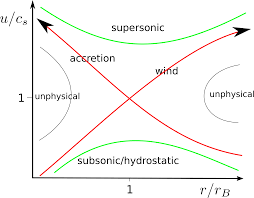
\includegraphics[width=0.75\linewidth]{Pictures/figures/bondi_regime.png}
    \caption{The parameter space of Bondi-accretion solutions. The sonic point $r_b$ is shown on the $x$-axis and the velocity on the $y$ axis.}
    \label{fig:bondi_regime}
\end{figure}
It is not immediately clear why we should have gone to all the work of building out this complicated ODE for ourselves; however, we can see that there are several very interesting features. The most important of these is that equation~\eqref{eq:bondi_critical_radius} is \textbf{singular} at 
\begin{equation}
    \label{eq:bondi_critical_radius}
    \boxed{
    r_s = \frac{GM}{2c_s^2}.
    }
\end{equation}
\rmk{Remember that $c_s$ is still a function of the radius. This means that this is \textbf{implicit}.} This is the so-called \textbf{sonic point} of the flow: \textit{if} the flow is going to make a transition to or from \textbf{sub-sonic} to \textbf{super-sonic}, it \textit{must occur at $r_s$.} This means that there are 4 important regimes to consider:
\vspace{0.5cm}
\begin{enumerate}
    \item \textbf{Transitioning Solution}: If we enforce that $u = c_s$ at the sonic radius, then the solution is entirely determined by the choice of behavior as $r\to \infty$ or by the choice of behavior as $r\to0$. If we let $u \to 0$ at $\infty$, then we obtain \textbf{accreting flows} featuring a transition point, and if we permit $u \to 0$ as $r\to 0$, then we obtain \textbf{wind flows} with transition points.
    \item \textbf{Non-Transitioning Solutions}: If a solution is not going to have $u=c_s$, then one \textit{must let $du^2/dr = 0$} at the sonic radius. In this case, the entire solution is fixed either by the behavior at either asymptote or by the behavior (the velocity) at the sonic point.
\end{enumerate}
\vspace{0.5cm}

\subsubsection{Bernoulli Flow}
We have now clarified the general behavior of the ODE we wish to solve and identified the relevant regimes. Most importantly, we are now able to recognize that uniqueness of our solution can be guaranteed by specifying the behavior both at the critical point and at $\infty$. Let us now fully solve the problem. To do so, we will apply \textbf{Bernoulli's Theorem}:
\[
u \frac{du}{dr}+ \nabla(h+\phi) = 0 \implies \frac{1}{2} u^2 + h + \phi = 0.
\]
For a \textbf{barotropic equation of state}, the specific enthalpy is
\[
h = \int \frac{dP}{\rho} = \int \frac{dP}{d\rho} \frac{1}{\rho} d\rho = \frac{K\gamma}{\gamma -1} \rho^{\gamma - 1} = \frac{c_s^2}{\gamma -1}.
\]
Thus,
\begin{equation}
    \frac{u^2}{2} + \frac{c_s^2}{\gamma -1} - \frac{GM}{r} = \rm{Constant}.
\end{equation}
\rmk{In the isothermal case, we actually need to have a logarithm here instead of $\gamma -1$.}
\par
Now, for \textbf{accreting flows}, we have $u(\infty) = 0$. Thus,
\[
c_s^2(\infty) = C(\gamma-1) \implies C = \frac{c_s^2(\infty)}{\gamma -1}.
\]
Additionally, the sonic point requires that
\[
c_s^2(r_s) = \frac{GM}{2r_s},
\]
so at $r_s$, we have
\[
\frac{c_s^2(r_s)}{2} + \frac{c_s^2(r_s)}{\gamma -1} - 2c_s^2(r_s) = \frac{c_s^2(\infty)}{\gamma -1}.
\]
So
\begin{equation}
\boxed{\
    c_s(r_s) = c_s(\infty) \left(\frac{2}{5 - 3\gamma}\right)^{1/2}
    }
\end{equation}
\rmk{NOTES: degeneracies!}
The mass accretion rate is constant at all radii, so we can evaluate it at the sonic point and find
\begin{equation}
    \boxed{
    \dot{M} = \pi G^2 M^2 \frac{\rho(\infty)}{c_s^3(\infty)} \left[\frac{2}{5-3\gamma}\right]^{(5-3\gamma)/2(\gamma-1)}.
    }
\end{equation}
\subsubsection{The Accretion Radius}

The Bondi solution motivates the introduction of a characteristic length scale, the
\textbf{accretion radius}, defined as
\begin{equation}
    \label{eq:bondi_radius}
    r_{\rm acc} \equiv \frac{2GM}{c_s^2(\infty)}.
\end{equation}
This can be understood from a simple energetic argument. At radius $r$, the
\textbf{gravitational binding energy per unit mass} is
\[
E_{\rm grav} \sim \frac{GM}{r},
\]
while the \textbf{thermal energy per unit mass} of the gas is set by the sound speed,
\[
E_{\rm th} \sim c_s^2(\infty).
\]
The radius $r_{\rm acc}$ is defined as the point where these two energy scales balance:
inside this radius, gravitational attraction dominates over thermal motions, so gas is
gravitationally captured by the accretor. Outside this radius, pressure forces can
support the gas against collapse. Thus, $r_{\rm acc}$ plays the role of an effective
``sphere of influence'' for accretion.

\begin{remark}
Note that $r_{\rm acc}$ is distinct from the precise sonic radius $r_s$, which depends
on the local sound speed $c_s(r_s)$. The accretion radius is defined in terms of the
\emph{asymptotic} sound speed at infinity, and provides a more intuitive, order-of-magnitude
measure of the capture region.
\end{remark}

\subsubsection{Free-Fall Behavior Beyond the Sonic Point}

Once the gas passes through the sonic point, the flow is \textbf{supersonic}. In this
regime, pressure forces are negligible compared to inertia and gravity: the gas
effectively undergoes free fall. This allows us to extract the asymptotic scaling of
velocity, density, and temperature in the inner region.

\paragraph{Velocity:} In free fall onto a point mass, the velocity is set by the
gravitational potential:
\[
u(r) \sim \left(\frac{2GM}{r}\right)^{1/2}.
\]

\paragraph{Density:} The accretion rate is constant at all radii,
\[
\dot{M} = 4\pi r^2 \rho u.
\]
Substituting the free-fall velocity,
\[
\rho(r) \sim \frac{\dot{M}}{4\pi r^2 u(r)} \;\propto\; r^{-3/2}.
\]

\paragraph{Temperature:} For a polytropic gas,
\[
T \propto \frac{P}{\rho} \propto \rho^{\gamma-1}.
\]
Thus, in the inner free-fall region,
\[
T(r) \;\propto\; r^{-3(\gamma-1)/2}.
\]
For example:
\begin{itemize}
    \item Isothermal case ($\gamma=1$): $T(r) = \rm{const}$.  
    \item Adiabatic monoatomic gas ($\gamma=5/3$): $T(r) \propto r^{-1}$.
\end{itemize}

\subsection{Feasibility as an Accretion Mechanism}

A natural question to ask is whether Bondi accretion can plausibly power luminous 
astrophysical phenomena such as X-ray binaries, ultraluminous X-ray sources (ULXs), 
or active galactic nuclei (AGN). The answer depends sensitively on the mass of the accretor 
and on the density and temperature of the ambient medium. 
\par
Let us consider first a \textbf{compact object} embedded in the 
interstellar medium (ISM). For typical ISM conditions, 
$n \sim 1\,{\rm cm^{-3}}$ and $T \sim 10^{4}\,{\rm K}$, the sound speed is of order 
$c_s \sim 10\,{\rm km\,s^{-1}}$. Substituting into the Bondi scaling,
\[
\dot{M}_{\rm Bondi} \;\sim\; 10^{12} 
\left(\frac{M}{M_\odot}\right)^2 \, {\rm g\,s^{-1}},
\]
we find accretion rates that correspond to luminosities
\[
L_{\rm acc} = \eta \dot{M} c^2 = 9\times 10^{32}\;\eta \left(\frac{M}{M_\odot}\right)^2 {\rm erg\;s^{-1}}
\]
where $\eta \sim 0.1$ is a typical accretion efficiency. For a \textbf{stellar mass} system, it is very hard to imagine scenarios in which this can work since $L_{\rm acc}$ might be as many as 10 magnitudes too low to explain the energetics of events like XRBs and ULXs. For \textbf{supermassive black holes}, the accretion can be considerably more energetic. For a $10^6$ solar mass black hole, we can already get up to $10^{45}\;{\rm erg \;s^{-1}}$, which puts us in range to explain AGN luminosity. \rmk{This is not actually the correct mechanism, however. We have said nothing yet of the emission mechanisms, which are also difficult to make work in the case of spherical accretion.}


\subsection*{Summary and Key Formulae}

Bondi accretion provides the simplest classical model for spherically symmetric accretion onto a compact object. While highly idealized, it illustrates several key physical principles:

\begin{itemize}
    \item The flow is uniquely determined by the requirement that it pass smoothly through the \textbf{sonic point}. This makes the solution transonic, subsonic at infinity and supersonic near the accretor. 
    \item The \textbf{accretion radius} 
    \[
    r_{\rm acc} = \frac{2GM}{c_s^2(\infty)}
    \]
    defines the natural scale inside which gravity dominates over thermal pressure. Gas at $r \lesssim r_{\rm acc}$ is gravitationally captured.
    \item The \textbf{Bondi accretion rate} can be expressed either in terms of $r_{\rm acc}$ or directly in terms of asymptotic conditions:
    \[
    \dot{M}_{\rm Bondi} \;\sim\; \pi r_{\rm acc}^2 \rho_\infty c_s(\infty),
    \qquad
    \dot{M}_{\rm Bondi} = \pi G^2 M^2 \frac{\rho(\infty)}{c_s(\infty)^3}\left[\frac{2}{5-3\gamma}\right]^{(5-3\gamma)/2(\gamma-1)}.
    \]
    The exact prefactor depends on the adiabatic index $\gamma$, but the scaling is robust.
    \item Inside the sonic point, the flow is effectively in free fall, with the following power-law scalings:
    \[
    u(r) \propto r^{-1/2}, \qquad \rho(r) \propto r^{-3/2}, \qquad T(r) \propto r^{-3(\gamma-1)/2}.
    \]
    For an adiabatic monoatomic gas ($\gamma=5/3$), this gives $T(r) \propto r^{-1}$.
    \item Order-of-magnitude estimates show that for compact objects, the rates are very small compared to what is observable:
    \[
    \dot{M}_{\rm Bondi} \sim 1.4 \times 10^{11}\;\; \left(\frac{M}{M_\odot}\right)^2 \left(\frac{\rho_\infty}{1\,{\rm cm}^{-3}\;m_p}\right)\left(\frac{10\,{\rm km/s}}{c_s(\infty)}\right)^3 \;{\rm g\,s^{-1}}.
    \]
    For example:
    \begin{itemize}
        \item White Dwarf ($M \sim 1M_\odot$, $R \sim 10^9\,$cm): $\dot{M} \sim 10^{12}\,{\rm g\,s^{-1}}$.
        \item Neutron Star ($M \sim 1.4M_\odot$, $R \sim 10^6\,$cm): $\dot{M} \sim 10^{13}\,{\rm g\,s^{-1}}$.
    \end{itemize}
    
Even though compact objects have deep gravitational potentials, the sparse interstellar medium is simply too dilute: Bondi accretion in realistic astrophysical settings is far below detectable levels.
\end{itemize}
\vspace{0.5cm}

\begin{bigidea}
\textbf{Bondi Accretion: Must-Remember Formulae}
\begin{align*}
r_{\rm acc} &= \frac{2GM}{c_s^2(\infty)} \\[6pt]
\dot{M}_{\rm Bondi} &\sim \pi r_{\rm acc}^2 \rho_\infty c_s(\infty) \;\;\;\; \propto \frac{(GM)^2 \rho_\infty}{c_s^3(\infty)} \\[6pt]
\rho(r) &\propto r^{-3/2}, \qquad T(r) \propto r^{-3(\gamma-1)/2}, \qquad u(r) \propto r^{-1/2} \\[6pt]
\dot{M}_{\rm WD} &\sim 10^{12} \;\left(\frac{M}{M_\odot}\right)^2\;{\rm g\,s^{-1}}, \qquad
\dot{M}_{\rm NS} \sim 10^{13} \;\left(\frac{M}{M_\odot}\right)^2\;{\rm g\,s^{-1}}
\end{align*}
\textbf{Takeaway:} Bondi accretion sets the baseline scale for spherical capture from a uniform medium, but the resulting accretion rates are far too small to be astrophysically significant in most environments.
\end{bigidea}

\begin{conceptbox}

Practical applications include:
\begin{itemize}
    \item Isolated neutron stars or black holes accreting from the interstellar medium.
    \item Quiescent supermassive black holes (e.g.\ Sgr A*) accreting from hot gas in galaxies.
    \item Wind-fed X-ray binaries, modeled with the related Bondi--Hoyle--Lyttleton formalism.
    \item Central black holes in galaxy clusters accreting from the intracluster medium.
    \item Subgrid prescriptions for black hole growth in cosmological simulations.
\end{itemize}
In each case, the Bondi rate provides an order-of-magnitude estimate of fuel availability, 
though real systems are often modified by angular momentum, turbulence, or feedback processes.
\end{conceptbox}

\section{Hoyle-Lyttleton Accretion}

- balistic characterization
- limitations.
- formalism

\subsection*{Summary and Key Formulae}

\section{Bondi-Hoyle-Lyttleton Accretion}

Summary and Key Formulae

\subsection{Issues with BHL Accretion}

\chapter{Binary Accretion}
Even more ubiquitous in astrophysics than accretion onto a single source is accretion between binary systems. This is also where we are able to learn the most about accretion because, by their nature, binary systems reveal more about themselves than individual systems do.
\par
In this section of notes, we'll work through the detailed geometry and dynamics of binary accretion mechanisms, which will lead us toward the theory of disk accretion.

\section{Dynamics of Binary Systems}

Before we dive into the fluid dynamics of binary accretion, we'll first discuss the dynamics of these systems from a gravitational standpoint. There are several important results and will come from this and help along the way later on.

\subsection{The Two-Body Problem}
To understand accretion in binary systems, it’s helpful to briefly recall the dynamics of the classical \textbf{two-body problem}.  We consider two point masses, $M_1$ and $M_2$, interacting only through gravity. Their positions relative to an inertial frame are ${\bf r}_1$ and ${\bf r}_2$, and the vector separating them is  
\[
{\bf r} = {\bf r}_2 - {\bf r}_1.
\]

The equations of motion are
\[
M_1 \ddot{\bf r}_1 = G \frac{M_1 M_2}{r^3} {\bf r}, 
\qquad
M_2 \ddot{\bf r}_2 = -G \frac{M_1 M_2}{r^3} {\bf r}.
\]
Adding these two gives conservation of the \textbf{center of mass (COM)}:
\[
M_1 \ddot{\bf r}_1 + M_2 \ddot{\bf r}_2 = 0 
\quad \Rightarrow \quad 
\ddot{\bf R}_{\rm COM} = 0,
\]
where 
\[
{\bf R}_{\rm COM} = \frac{M_1 {\bf r}_1 + M_2 {\bf r}_2}{M_1 + M_2}.
\]
It is therefore natural to work in the COM frame, where ${\bf R}_{\rm COM} = 0$.  
Defining the \textbf{reduced mass} 
\[
\mu = \frac{M_1 M_2}{M_1 + M_2},
\]
the relative motion reduces to a single particle of mass $\mu$ moving under the potential of the total mass $M = M_1 + M_2$:
\[
\mu \ddot{\bf r} = - \frac{G M_1 M_2}{r^3} {\bf r}
\quad \Rightarrow \quad 
\ddot{\bf r} = - \frac{G M}{r^3} {\bf r}.
\]
Thus, the two-body problem reduces to the motion of a single body in a central potential.  
The orbits are conic sections—elliptical for bound systems—with angular momentum per unit mass
\[
{\bf L} = {\bf r} \times \dot{\bf r},
\]
and total specific energy
\[
E = \frac{1}{2}\dot{r}^2 - \frac{GM}{r}.
\]
While this is a fairly elementary problem to solve and is well known to most astronomy students, it is worth noting that our standard intuition for orbits must be stretched somewhat in this case. We now recognize that it is the \textbf{separation} between the two bodies which follows a standard elliptical orbit and that we must be careful not to mistake our intuition for planetary orbits with those here.
\par
Now, the \textbf{main observable of a binary is the period}, therefore, we will use that to determine other properties. Using \textbf{Kepler's Law},
\[
a^3 = \frac{GM_{\rm tot}}{4\pi^2} P^2.
\]
\rmk{It's worth remembering here that this is the \textit{relative orbit} in the equivalent 1-body problem. Thus, its the proper distance \textit{between the companions}, but it is NOT the orbital radius.}
We will also find it convenient to introduce the \textbf{mass ratio} $q = M_2/M_1$. We may write $a$ in terms of the mass ratio and the period as
\begin{equation}
\label{eq:binary_orbit_semi_major_axis}
\boxed{
    a = \left(\frac{G}{4\pi^2}\right)^{1/3} M_1^{1/3}(1+q)^{1/3} P^{2/3}.
}
\end{equation}
In units of solar masses, this reduces to
\begin{equation}
    \label{eq:binary_orbit_semi_major_axis_united}
    \boxed{
    a = \begin{cases}
        1.5\times 10^{13} \left(\frac{M_1}{M_\odot}\right)^{1/3} (1+q)^{1/3} P_{\rm years}^{2/3}\; {\rm cm},&\\
                2.9\times 10^{11} \left(\frac{M_1}{M_\odot}\right)^{1/3} (1+q)^{1/3} P_{\rm days}^{2/3}\; {\rm cm},&\\
                        3.5\times10^{10} \left(\frac{M_1}{M_\odot}\right)^{1/3} (1+q)^{1/3} P_{\rm hrs}^{2/3}\; {\rm cm},&\\
    \end{cases}
    }
\end{equation}
\begin{remark}
    Notice that $q > 0$ no matter what, so we always know that leaving out the $1+q$ term provides a \textbf{lower bound} on $a$. In principle, $q \to \infty$ can occur, in which case $a \to \infty$; however, this isn't really relevant in practice.
\end{remark}

In the COM frame, the distance to each of the companions is determined by the fact that ${\bf r} = {\bf r}_1 - {\bf r}_2 = a$, which means that (\rmk{easy enough to work this out from the definition of the COM}),
\[
{\bf r}_1 = \frac{M_2}{M_1+M_2} {\bf r},\; {\bf r}_2 = - \frac{M_1}{M_1+M_2} {\bf r}.
\]
In terms of $q$, 
\[
{\bf r}_1 = \frac{1}{1+q} {\bf r},\; {\bf r}_2 = - \frac{q}{1+q} {\bf r}.
\]


\subsection{Tidal Forces in Binary Systems}

One important feature of accreting binaries is that they are \textbf{close binaries}: therefore, we cannot ignore the role that tidal forces play in the dynamics. This serves two really important purposes which we will exploit in developing the theory:

\begin{enumerate}
    \item Tidal forces \textbf{circularize binary orbits}, and
    \item tidal forces \textbf{synchronize axial rotations}.
\end{enumerate}

To understand these phenomena, we consider a qualitative picture: Let $M_1$ and $M_2$ be the masses of two stars in binary orbit. If $M_1$ experiences tidal distortion, it will bulge along the \textit{line of centers}. Now, the star is also rotating, which means that the bulge will need to shift backward to align with the line of centers. In a perfectly elastic star, this shift could happen rapidly, but that is not generally the case. 
\par
As a result, the tidal bulge tends to either lead or follow the \textit{line of centers}, which means that the COM of the star is shifted either forward or backward in the orbit. If it is shifted backward, then the companion will pull it forward, slowing the rotation and increasing the angular momentum in the orbit to match. Likewise, if it is shifted forward, it will be pulled backward and the rotation will increase and angular momentum will be pulled out of the orbit. Internally, this rearranging of material will lead to dissipative processes which serve to reduce the overall energy of the orbit to the minimum possible for a given fixed angular momentum. This will correspond to synchronous rotation of the binaries and circular orbits.
\par
In general, this process is quite efficient:
\[
t_{\rm tide} \sim \left(\frac{a}{R}\right)^5\;\text{or faster},
\]
where $a$ is the semi-major axis of the orbit and $R$ is the radius of the tidally effected star. It is therefore \textit{generally} the case that these evolutions occur on time scales short relative to the timescale of accretion.
\rmk{(This is not \textit{always} the case: there are exceptions!)}
\paragraph{Implications}
The result of this is that, for most relevant systems, we can treat the problem of accretion in a somewhat simpler scenario: we have circular, Keplerian orbits and the systems are tidally locked. This means that in a frame centered on the COM and co-rotating with the orbit, the bodies appear to be \textbf{stationary}.

\subsection{The Restricted 3-Body Problem}

Having established the dynamics of the two companion stars, we now ask a natural question:
\vspace{0.25cm}
\begin{center}
    \textit{What is the motion of a test particle released in the combined gravitational field of the two companions?}
\end{center}
\vspace{0.25cm}

To study this problem, we work in the \textbf{co-rotating center-of-mass frame}. In this frame, the two companions remain \textbf{fixed} at their orbital radii and appear \textbf{non-rotating}. The tradeoff is that we must introduce the \textbf{fictitious forces} associated with the non-inertial frame. Defining the rotational velocity vector
\[
\boldsymbol{\Omega} = \Omega \hat{\bf z} 
= \left(\frac{GM}{a^3}\right)^{1/2}\hat{\bf z},
\]
the fictitious accelerations are:
\vspace{0.5cm}
\begin{enumerate}
    \item \textbf{Coriolis Force}: ${\bf F}_{\rm cor} = -2m\, \boldsymbol{\Omega} \times \dot{\bf r}$,
    \item \textbf{Centrifugal Force}: ${\bf F}_{\rm cent} = -m\, \boldsymbol{\Omega} \times (\boldsymbol{\Omega} \times {\bf r})$,
    \item \textbf{Euler Force}: ${\bf F}_{\rm Euler} = -m\, \dot{\boldsymbol{\Omega}} \times {\bf r}$.
\end{enumerate}
\vspace{0.5cm}

For binaries of constant orbital period, $\dot{\boldsymbol{\Omega}}=0$, so the Euler force can be neglected. The Euler equation in the rotating frame becomes
\[
\frac{D{\bf u}}{Dt} = - \frac{\nabla P}{\rho} - \nabla \Phi_{\rm Roche} - \underbrace{2 \boldsymbol{\Omega} \times \dot{\bf r}}_{\text{Coriolis Force}},
\]
where $\Phi_{\rm Roche}$ is the combined gravitational and centrifugal potential, called the \textbf{Roche Potential}:
\begin{equation}
    \label{eq:roche_potential}
    \boxed{
    \Phi_{\rm Roche} =
    - GM_2 \left[\frac{1}{q|{\bf r} - {\bf r}_1|} + \frac{1}{\,|{\bf r}-{\bf r}_2|}\right]
    - \tfrac{1}{2}\left|\boldsymbol{\Omega}\times{\bf r}\right|^2
    }.
\end{equation}

\begin{figure}
    \centering
    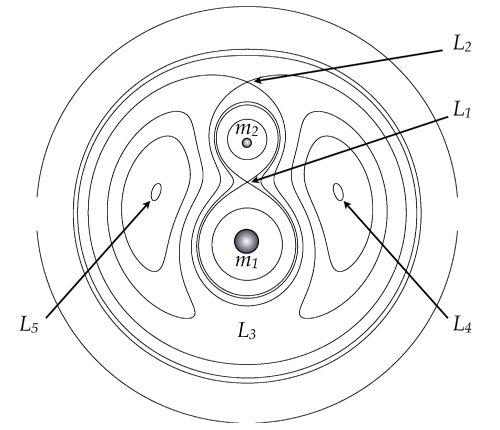
\includegraphics[width=0.75\linewidth]{Pictures/figures/roche_potential.png}
    \caption{The Roche potential in the orbital plane for a representative mass ratio. Equipotential contours illustrate the balance between gravitational and centrifugal forces in the co-rotating frame.}
    \label{fig:roche_potential}
\end{figure}

\subsubsection{Lagrange Points}

Inspection of the Roche potential (Figure~\ref{fig:roche_potential}) reveals the existence of \textbf{five equilibrium points}, known as the \textbf{Lagrange points}. At these locations, the effective force vanishes in the co-rotating frame. Of these, the most important for mass transfer is the inner point, $L_1$, located between the two stars. This is a \textbf{saddle point} of the potential and defines the boundary between the two \textbf{Roche lobes}. Material within a lobe is gravitationally bound to its host star, while material near $L_1$ can pass through to the companion. 

In two dimensions, the Roche lobes take the form of a figure-eight, while in three dimensions they resemble a dumbbell (Figure~\ref{fig:roche_lobes}). The geometry of these lobes determines when a star will begin to lose mass through Roche lobe overflow.

\begin{figure}
    \centering
    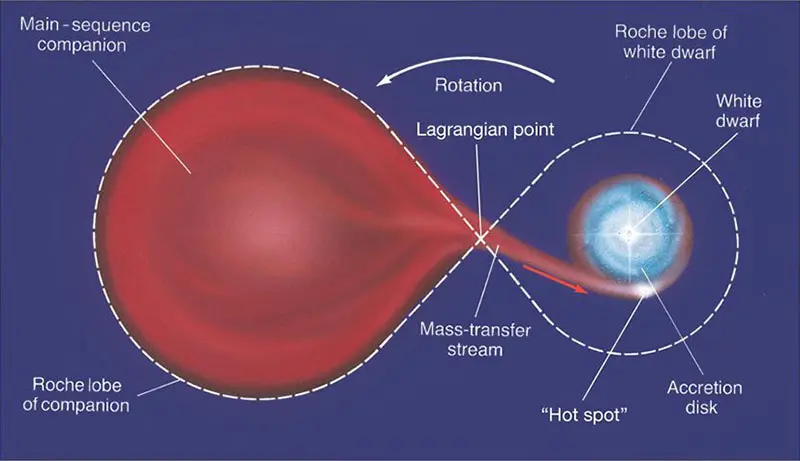
\includegraphics[width=0.75\linewidth]{Pictures/figures/roche_lobes.png}
    \caption{The Roche lobes of two stars in a binary, shown as equipotential surfaces of the Roche potential. The $L_1$ point at the intersection of the lobes sets the critical condition for Roche lobe overflow.}
    \label{fig:roche_lobes}
\end{figure}

\section{Roche Lobe Overflow}

We now discuss the nature of material accreted onto a companion from a progenitor star. Consider the scenario given above when the radii of the individual companions ($R_1$ and $R_2$) are each much, much smaller that their respective Roche Lobes. From the Euler Equation,
\[
\frac{D{\bf u}}{Dt} = - \frac{\nabla P}{\rho} - \nabla \Phi_{\rm Roche} - 2 \boldsymbol{\Omega} \times {\bf u},
\]
we see that in steady state,
\[
0 = - \frac{\nabla P}{\rho} - \nabla \Phi_{\rm Roche},
\]
which implies that the surface (defined by $\nabla P = 0$) will coincide with one of the inner most equipotentials deep within the respective Roche lobe. What do we learn from this? \textbf{For binaries which are each deep within their own Roche Lobes, there is no impetus for mass transfer.} Such binaries are called \textbf{detached binaries}.
\par
Now we might consider another scenario where one companion (the so-called \textbf{secondary} or \textbf{non-accretor}) expands (due to any number of relevant processes) such that it begins to fill its Roche Lobe. Here's the critical idea:
\vspace{0.25cm}
\begin{center}
    When material on the surface (which is on equipotentials of $\Phi_{\rm Roche}$) begins to fill the Roche-Lobe, that material will lie close to the $L_1$ point. In turn, perturbations can \textbf{displace material across $L_1$ into the corresponding Roche Lobe of the primary WITHOUT needing additional energy input.} 
\end{center}
\vspace{0.25cm}
Such binaries are called \textbf{semi-detached binaries} and are able to efficiently transfer mass across the $L_1$ point. Another interesting scenario occurs when both objects fill their Roche-Lobes, creating a so-called \textbf{contact binary}.
\begin{remark}
    It will be seen that the rate of material flow is quite fast. As such, we rarely get a companion which is much larger than its own Roche Lobe.
\end{remark}

\subsection{Geometry of Binary Accretion}

Before we can work out the details of binary accretion, we'll need to do a bit of geometry. Our goal here is to answer the following general questions:
\vspace{10pt}
\begin{enumerate}
    \item \textbf{Where} is the L1 point relative to the primary in a binary system?
    \item \textbf{How big} is the Roche Lobe for a given mass?
    \item \textbf{What} determines the size and shape of the Roche Lobe?
\end{enumerate}
\vspace{10pt}
\medskip
\par
Looking again at the equation for the Roche Potential, we have \eqref{eq:roche_potential}
\[
    \Phi_{\rm Roche} =
    - GM_2 \left[\frac{1}{q|{\bf r} - {\bf r}_1|} + \frac{1}{\,|{\bf r}-{\bf r}_2|}\right]
    - \tfrac{1}{2}\left|\boldsymbol{\Omega}\times{\bf r}\right|^2.
\]
If we imagine that the binary orbit is circular, then their distance is determined unambiguously from their period (or, conversely, their period is determined from their distance). As such, we see that there are only really two major ingredients in determining the scale and shape of the Roche Lobes:
\vspace{10pt}
\begin{enumerate}
    \item The \textbf{separation} determines a scale for the Roche Geometry,
    \item The \textbf{mass ratio} determines the shape of the geometry.
\end{enumerate}
\vspace{10pt}
The implication here is quite clear: we \textbf{should} be able to say a great deal about the geometry of the Roche System without a direct reference to anything other than $q$. Unfortunately, it is generally a task requiring numerical solution, but there are some quasi-analytic formulae which will be relevant to our discussion of these phenomena.

\subsubsection{The Roche Lobe Radius}

One such option is the \textbf{Eggleton Formula}, which dictates the \textbf{shape of the Roche Lobe} as a function of the mass ratio $q$. It is a numerical fit to computation data taking the form:
\begin{equation}
\label{eq:eggleton_formula}
\boxed{
    \frac{R_2}{a} = \frac{\alpha q^{2/3}}{\beta q^{2/3} + \log(1+q^{1/3})}
    }
\end{equation}
where $\alpha = 0.49$, and $\beta = 0.6$. \rmk{We can get at $R_1$ from replacing $q$ with $q^{-1}$.} Here, $R_2$ is the \textit{effective radius} of the lobe defined as the radius of a sphere with the \textit{same volume as the lobe.} There are also two other approximations worthy of mention:

\begin{enumerate}
    \item $(0.1 \le q \le 0.8)$: We can use a simplified version from \citet{1971ARA&A...9..183P}:
    \begin{equation}
        \label{eq:paczynski_lobe_radius}
        \boxed{
        \frac{R_2}{a} = \frac{2}{3^{4/3}}\left(\frac{q}{1+q}\right)^{1/3} = 0.462\left(\frac{M_2}{M_1+M_2}\right)^{1/3}.}
    \end{equation}
This proves to be a \textbf{massively important} equation because it permits us to discuss many different scaling relationships for different types of primaries and secondaries.
    \item $(0.03 < q < 1)$ also allows
\[
\frac{R_1}{R_2} = \left(\frac{M_1}{M_2}\right)^{0.45}.
\]

\end{enumerate}

\subsubsection{The Location of the Lagrange Point}

We are also interested in the distance between the \textit{primary} (the accretor) and the Roche-Lobe critical point. To good accuracy, a fitted formula suffices \citep{1964BAICz..15..165P}:
\begin{equation}
    \label{eq:roche_overflow_distance}
    \frac{b_1}{a} = 0.5 - 0.227 \log q,
\end{equation}
where $a$ is the semi-major axis (the distance between the primary and the secondary due to circularization) and $b_1$ is the distance between the primary and the Roche point. Clearly, for $q = 1$, the Roche point is right between the primary and the secondary. For $q \gg 1$ (corresponding to a low mass accretor and high mass donor), the overflow point get \textbf{closer to the primary} since the secondary can bind material more effectively. In the opposite scenario, $q \ll 1$, the overflow point gets closer to the secondary. To \textbf{first order} in $q$, this is
\[
\frac{b_1}{a} \approx 0.5 - 0.227(q-1).
\]
\subsection{Scaling Relations for Roche Lobe Overflow}

One of the most useful aspects of equation~\eqref{eq:paczynski_lobe_radius} is that it expresses the Roche–lobe radius $R_2$ entirely in terms of the binary separation $a$ and the mass ratio $q = M_2 / M_1$.  
Using Kepler’s Third Law, we can replace the separation by the observable orbital period $P$:
\begin{equation}
a = \left[\frac{G (M_1 + M_2)}{4\pi^2}\right]^{1/3} P^{2/3}.
\end{equation}
Substituting into the Roche–lobe relation gives
\begin{align}
R_2 &\approx a\,\frac{2}{3^{4/3}} \left(\frac{q}{1+q}\right)^{1/3} \\[4pt]
&= \frac{2}{3^{4/3}}\!\left(\frac{G}{4\pi^2}\right)^{1/3}
   P^{2/3} (M_1 + M_2)^{1/3}
   \left(\frac{M_2}{M_1 + M_2}\right)^{1/3} \\[4pt]
&= \frac{2}{3^{4/3}}\!\left(\frac{G}{4\pi^2}\right)^{1/3}
   P^{2/3} M_2^{1/3}.
\end{align}
Thus, to good approximation, the Roche–lobe radius of the donor depends only on its own mass and the binary period.  
Evaluating the constants yields the very useful scaling:
\[
\boxed{
R_2 \simeq 6.2 \times 10^{11}
\left(\frac{P}{{\rm 1\,day}}\right)^{2/3}
\left(\frac{M_2}{M_\odot}\right)^{1/3}
{\rm cm}.
}
\]

\subsubsection{The Period–Density Relation}

Since a Roche–lobe filling star must satisfy this radius–period relation, its mean density follows immediately:
\begin{equation}
\bar{\rho} = \frac{3M_2}{4\pi R_2^3}.
\end{equation}
Substituting for $R_2$, we find
\begin{align}
\bar{\rho} 
   &\sim \frac{3M_2}{4\pi}
      \left[\frac{3^{4/3}}{2}
      \left(\frac{4\pi^2}{G}\right)^{1/3}
      P^{-2/3} M_2^{-1/3}\right]^3 \\[4pt]
   &= \frac{3^5 \pi}{8 G P^2}.
\end{align}
Hence the donor’s mean density depends \emph{only on the orbital period}, not on the stellar mass or composition:
\[
\boxed{
\bar{\rho} \;\approx\; 110\,P_{\rm hr}^{-2}\;{\rm g\,cm^{-3}},
}
\]
where $P_{\rm hr}$ is the orbital period in hours.

\medskip
\noindent
\textbf{Physical meaning:} systems with shorter periods must contain denser donors.  
This simple $P^{-2}$ scaling makes the orbital period a direct diagnostic of the donor’s mean density—and thus its evolutionary state.

\subsubsection{The Mass–Period Relation for Polytropic Donors}

If the donor follows a polytropic structure with index $n$, then
\begin{equation}
R \propto M^{\frac{1-n}{3-n}},
\end{equation}
and the corresponding mean density is
\begin{equation}
\bar{\rho} \propto M^{\tfrac{3n}{3-n}}.
\end{equation}
Since Roche–lobe filling enforces $\bar{\rho} \propto P^{-2}$, we obtain the general
\textbf{mass–period relation}:
\[
\boxed{
P \propto M^{-\tfrac{3n}{2(3-n)}}.
}
\]

\paragraph{Main Sequence Donors}
For main sequence stars, an empirical relation $R \propto M^{3/4}$ is a good approximation.  
Then
\begin{align}
\bar{\rho}
   &= \frac{3M}{4\pi R^3}
   \approx 1.4
   \left(\frac{M}{M_\odot}\right)^{-5/4}
   {\rm g\,cm^{-3}},
\end{align}
and equating with $\bar{\rho} \approx 110\,P_{\rm hr}^{-2}$ gives
\[
P_{\rm hr} \approx 8.8
\left(\frac{M}{M_\odot}\right)^{5/8},
\qquad
\boxed{
\frac{M}{M_\odot} \approx 0.03\,P_{\rm hr}^{8/5}.
}
\]
Because main sequence stars cannot exist below about $0.1\,M_\odot$, this relation implies a lower limit near 
$P_{\rm min} \sim 2\,{\rm hr}$—shorter-period systems must therefore contain evolved or degenerate donors.

\paragraph{Degenerate Donors}
For fully degenerate (non-relativistic) donors, $R \propto M^{-1/3}$, so that
\[
\bar{\rho} \propto M^{2},
\qquad
P \propto M^{-1}.
\]
Hence more massive degenerate donors correspond to shorter orbital periods.  
A typical scaling is
\[
\boxed{
P_{\rm sec} \approx 150
\left(\frac{M}{M_\odot}\right)^{-1},
}
\]
appropriate for low-mass white dwarf donors.

\subsubsection{The Minimum Period in Compact Binaries}

These two contrasting mass–period scalings explain the observed \textbf{period bounce} in compact binaries:
\begin{itemize}
    \item For \textbf{main sequence donors} ($R \propto M^{3/4}$):  
    $P \propto M^{8/5}$, so as mass is lost, the orbital period \emph{decreases}.
    \item For \textbf{degenerate donors} ($R \propto M^{-1/3}$):  
    $P \propto M^{-1}$, so further mass loss causes the period to \emph{increase}.
\end{itemize}
The system therefore evolves toward shorter periods until the donor becomes degenerate, reaches a minimum period, and then expands again.  
This transition defines the \textbf{minimum orbital period}:
\[
P_{\rm min} \sim 1\,{\rm hr}, 
\qquad
M_2 \sim 0.03\text{--}0.04\,M_\odot.
\]

\begin{bigidea}
\textbf{Key Concepts}
\begin{itemize}
    \item The Roche–lobe size depends only on the mass ratio $q$ and separation $a$.
    \item For a Roche–lobe filling star, the \textbf{mean density depends solely on the orbital period}:
    \[
    \bar{\rho} \approx 110\,P_{\rm hr}^{-2}\;{\rm g\,cm^{-3}}.
    \]
    \item Combining this with stellar structure relations $R(M)$ gives characteristic \textbf{mass–period laws}:
    \begin{itemize}
        \item \textbf{Main sequence donors:} $P_{\rm hr} \approx 8.8(M/M_\odot)^{5/8}$.
        \item \textbf{Degenerate donors:} $P_{\rm sec} \approx 150(M/M_\odot)^{-1}$.
    \end{itemize}
    \item The \textbf{period bounce} arises where these two regimes meet, marking the transition from main sequence to degenerate donors.
\end{itemize}
\end{bigidea}

\subsection{The Evolution of Binary Systems}

The evolution of a binary system is governed by the exchange of two fundamental quantities:
\textbf{mass} and \textbf{angular momentum}.  
Any process that redistributes or removes either quantity inevitably alters the orbital configuration of the system—often in a way that feeds back on the rate and stability of mass transfer itself.

\par
In most cases, we begin by assuming \textbf{conservative mass transfer}, in which the mass lost by the donor (secondary) is entirely accreted by the companion (primary). However, it is not always valid to assume that the system’s \textbf{angular momentum} is likewise conserved. Angular momentum losses can profoundly affect the orbital evolution and often determine whether mass transfer proceeds stably or becomes dynamically unstable.

\begin{definition}[Fully Conservative Mass Transfer]
\textbf{Fully conservative mass transfer} refers to the idealized case in which both the total mass and the total angular momentum of the binary are conserved:
\[
\dot{M}_1 + \dot{M}_2 = 0, \qquad \dot{J} = 0.
\]
In this limit, all material lost by the donor is accreted by the companion, and no angular momentum escapes the system.
\end{definition}

\par
In reality, few binaries are perfectly conservative.  Mass and angular momentum can be lost through several mechanisms—most notably through \textbf{gravitational wave radiation}, \textbf{stellar winds}, or \textbf{magnetically driven outflows}.  These processes remove energy and angular momentum from the orbit, driving secular changes in the separation and period that ultimately shape the system’s long-term evolution.
\medskip
\noindent
As we will see in the sections that follow, the coupled transfer of mass and angular momentum governs the fate of a binary system—determining whether it expands or contracts, remains stable, or undergoes runaway mass transfer leading to a common-envelope phase.

\subsubsection{The Role of Angular Momentum}

Given an orbital period $P$ and angular velocity $\omega = 2\pi / P$, the total orbital angular momentum is
\[
J = (M_1 a_1^2 + M_2 a_2^2)\,\omega,
\]
where $a_1$ and $a_2$ are the distances of each component from the center of mass:
\[
a_1 = \frac{M_2}{M_1 + M_2}a,
\qquad
a_2 = \frac{M_1}{M_1 + M_2}a.
\]
Substituting these expressions and invoking Kepler’s third law,
\[
\omega^2 a^3 = G(M_1 + M_2),
\]
we obtain the compact and widely used form:
\[
\boxed{
J = M_1 M_2 \left(\frac{G a}{M_1 + M_2}\right)^{1/2}.
}
\]
If we now take the \textbf{logarithmic derivative} of the above equation, we find after requiring \textbf{conservative mass transfer} that
\begin{equation}
    \label{eq:ang_mom_binary_ev}
\frac{\dot{a}}{a} = \frac{2\dot{J}}{J}
    + 2\frac{(-\dot{M}_2)}{M_2}\left(1 - \frac{M_2}{M_1}\right),
\end{equation}
which leads us immediately to a big idea:
\begin{bigidea}

Equation~\eqref{eq:ang_mom_binary_ev} shows how the \textbf{orbital separation $a$} responds to changes in angular momentum and mass transfer! From this expression, we can immediately draw several key conclusions:
\begin{itemize}
    \item If \textbf{angular momentum is conserved} ($\dot{J}=0$):
    \begin{itemize}
        \item When $M_2 < M_1$, the factor $(1 - M_2/M_1)$ is positive, so $\dot{a} > 0$.  
        The orbit \textbf{expands} as the lighter donor transfers mass to the heavier accretor.
        \item When $M_2 > M_1$, the factor $(1 - M_2/M_1)$ is negative, so $\dot{a} < 0$.  
        The orbit \textbf{shrinks} as the more massive star loses mass to its lighter companion.
    \end{itemize}
    \item If \textbf{angular momentum is lost} ($\dot{J}<0$), this term always contributes to orbital contraction, regardless of the mass ratio.  
\end{itemize}
An intuitive way to think about this is in the limit $q \gg 1$, in which case we are just adding mass or removing mass from a mass on a string. If we add mass, we would need to swing harder
to keep it at the same distance, or we would shorten the string. Likewise, if we remove mass, it will want to drift outward.
\end{bigidea}

\medskip
\paragraph{Angular Momentum Loss Channels.}
In the idealized \emph{fully conservative} case, the total angular momentum of the system is conserved ($\dot{J}=0$).  
However, in realistic binaries, a variety of processes can remove angular momentum from the orbit.  
These losses drive secular changes in the orbital separation and can dramatically influence the stability of mass transfer.  
The most important loss mechanisms are summarized below.

\begin{itemize}
    \item \textbf{Gravitational Radiation.}  
    Compact binaries (white dwarfs, neutron stars, black holes) emit gravitational waves as they orbit, carrying away angular momentum at a rate
    \[
    \dot{J}_{\rm GW} = -\frac{32}{5}\frac{G^{7/2}}{c^5}
        \frac{M_1^2 M_2^2 (M_1 + M_2)^{1/2}}{a^{7/2}}.
    \]
    This loss steeply depends on $a^{-7/2}$, making gravitational radiation dominant only in very tight systems.  
    The resulting orbital decay leads to a gradual inspiral, eventually producing a merger or the onset of Roche–lobe overflow.

    \item \textbf{Magnetic Braking.}  
    In systems containing late-type (cool, convective) stars, magnetic fields can couple the stellar wind to the star’s rotation.  
    The wind carries away angular momentum from the spin of the donor, which is tidally locked to the orbit.  
    As a result, the \emph{orbital} angular momentum also decreases.  
    The torque can be approximated by empirical laws such as
    \[
    \dot{J}_{\rm MB} \propto - M_2 R_2^{4} \omega^{3},
    \]
    though the efficiency depends strongly on the magnetic field geometry and wind strength.  
    Magnetic braking is a key driver of orbital evolution in cataclysmic variables and low-mass X-ray binaries.

    \item \textbf{Stellar Winds and Outflows.}  
    When one or both stars lose mass in a stellar wind, the escaping gas carries with it specific angular momentum.  
    The total angular momentum loss depends on where the mass leaves:
    \[
    \dot{J}_{\rm wind} \sim \dot{M}_{\rm loss}\, a^2 \omega.
    \]
    If the lost material escapes isotropically from the system, the orbit typically \emph{expands}; if it leaves preferentially through $L_2$ or in a focused jet, it can instead lead to orbital contraction.

    \item \textbf{Mass Loss through $L_2$ or a Circumbinary Disk.}  
    When transfer through $L_1$ becomes excessive, material may flow out through the outer Lagrange point $L_2$, forming a circumbinary ring or disk.  
    Because this ejected matter orbits at larger radii, it extracts \emph{more} specific angular momentum per unit mass than the binary average, leading to rapid orbital decay and possibly a common-envelope phase.

    \item \textbf{Tidal Torques and Spin–Orbit Coupling.}  
    In close systems, tidal interactions exchange angular momentum between the stellar spins and the orbit.  
    Tidal friction tends to synchronize rotation and circularize the orbit.  
    If either star contracts or expands (changing its moment of inertia), this coupling can further exchange angular momentum with the orbit.
\end{itemize}

\paragraph{Consequences of Angular Momentum Loss.}
All of these processes modify the orbital separation through the relation
\[
\frac{\dot{a}}{a} = \frac{2\dot{J}}{J}
    - 2\frac{\dot{M}_2}{M_2}\left(1 - \frac{M_2}{M_1}\right),
\]
which shows that $\dot{J}<0$ always drives orbital contraction.  
In compact systems, this can bring the stars into contact and trigger Roche–lobe overflow, while in wider systems it may gradually shrink the orbit over gigayear timescales.

\begin{bigidea}
\textbf{Angular Momentum Loss Summary}
\begin{itemize}
    \item \textbf{Gravitational waves} dominate at small separations ($a \lesssim R_\odot$).
    \item \textbf{Magnetic braking} dominates for cool, magnetized donors in wider binaries.
    \item \textbf{Winds and circumbinary mass loss} remove angular momentum at intermediate scales and often govern long-term orbital evolution.
    \item \textbf{Tidal coupling} redistributes angular momentum between spin and orbit, enforcing synchronization and circularization.
\end{itemize}
Together, these mechanisms determine whether a binary will widen, shrink, or merge—and hence whether it becomes a stable accretor, a contact binary, or a gravitational wave source.
\end{bigidea}

\subsection{Mass Transfer Stability}
\begin{figure}[ht!]
    \centering
    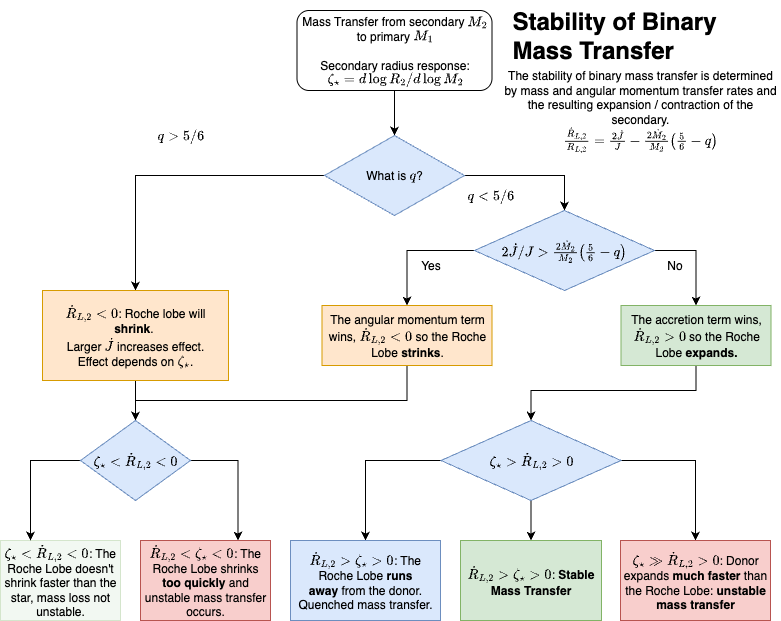
\includegraphics[width=1\linewidth]{Pictures/figures/binary_mass_accretion.png}
    \caption{The various modes of binary mass transfer and the resulting stability as dictated by the stellar contraction response, $\zeta_\star$ and the contraction of the donor Roche Lobe. This is characterized by equation~\eqref{eq:roche_lobe_stability}.}
    \label{fig:roche_transfer_stability}
\end{figure}

Let's now ask the following question: \textbf{what happens to the Roche Lobe when mass is transferred?} 
From equation~\eqref{eq:paczynski_lobe_radius}, we can logarithmically differentiate to find
\[
\boxed{
\frac{\dot{R}_2}{R_2} = \frac{\dot{a}}{a} + \frac{\dot{M}_2}{3M_2},
}
\]
which can then be substituted into \eqref{eq:ang_mom_binary_ev} to obtain
\begin{equation}
\label{eq:roche_lobe_stability}
\boxed{
    \frac{\dot{R}_2}{R_2} = \frac{2\dot{J}}{J} - \frac{2\dot{M}_2}{M_2}\left(\frac{5}{6}-\frac{M_2}{M_1}\right).
}
\end{equation}
\par
We can now interpret equation~\eqref{eq:ang_mom_binary_ev}
together with the Roche lobe response.  The key diagnostic is
\[
\frac{\dot{R}_2}{R_2} = \frac{2\dot{J}}{J}
   + \frac{2(-\dot{M}_2)}{M_2}\!\left(\frac{5}{6} - \frac{M_2}{M_1}\right),
\]
which measures how the Roche lobe of the donor responds as mass is lost.

\begin{enumerate}
    \item \textbf{Unstable (Cataclysmic) Mass Transfer, $q > 5/6$:}  
    In this regime the second term on the right--hand side is negative.  
    If there is any angular momentum loss ($\dot{J}<0$), the Roche lobe shrinks as material is lost.  
    The donor thus overfills its Roche lobe more and more, leading to a runaway process.  
    This behavior underlies cataclysmic variables and other explosive transfer scenarios.

    \item \textbf{Stable Mass Transfer, $q < 5/6$:}  
    Here the second term tends to be positive, so the Roche lobe expands as mass is removed.  
    Provided angular momentum loss is not too strong, the Roche lobe expansion can keep pace with 
    the donor’s radius, allowing for long--lived, secular mass exchange on nuclear or thermal timescales.  

    \item \textbf{Role of Angular Momentum Loss:}  
    Even for $q > 5/6$, strong angular momentum loss (e.g.\ by gravitational radiation or magnetic braking) 
    can still cause the Roche lobe to contract, destabilizing the system.  
    Conversely, with $\dot{J}=0$ and $q > 5/6$, mass transfer remains stable.
\end{enumerate}

\noindent
Thus the fate of the binary depends jointly on the \emph{mass ratio} and the \emph{angular momentum loss channels}:  
low-$q$ systems tend toward runaway transfer, while high-$q$ systems may support stable, long-lived exchange.

\begin{bigidea}
    From the discussion above, we have two very useful criteria which tell us \textbf{a lot} about the nature of our accretion.
    \begin{enumerate}
        \item The equation
            \[ 
            \frac{\dot{a}}{a} = \frac{2\dot{J}}{J} - \frac{2 \dot{M}_2}{M_2} \left(1-\frac{M_2}{M_1}\right)
            \]
            derived above gives us a clear threshold for the \textbf{expansion / contraction} of the orbits:
            \begin{itemize}
                \item If $M_2>M_1$, then the orbit will \textbf{shrink}.
                \item If $M_1 > M_2$, then the orbit will \textbf{expand}.
            \end{itemize}
            Thus, the stability of the binary depends crucially on the initial mass ratio.
        \item Using the Paczyński approximation, we also know that 
        \[
        \frac{\dot{R}_2}{R_2} = \frac{2\dot{J}}{J} - \frac{2\dot{M}_2}{M_2}\left(\frac{5}{6}-\frac{M_2}{M_1}\right),
        \]
        which tells us how the Roche lobe radius evolves relative to the donor mass. 
        \begin{itemize}
            \item If $\frac{M_2}{M_1} < \tfrac{5}{6}$, then (because $\dot{M}_2 < 0$), the second term on the RHS provides a \textbf{positive contribution} and therefore generally leads to Roche Lobe \textbf{expansion} unless $\dot{J}$ is \textbf{very large}. This is the regime where stable mass transfer can occur.
            \item If $\frac{M_2}{M_1} > \tfrac{5}{6}$, then the coefficient of $\dot{M}_2$ is negative, and the Roche lobe radius \textbf{shrinks}. This drives \textbf{unstable}, runaway mass transfer.
            \item Angular momentum losses ($\dot{J}<0$) further reduce $R_2$, making instability \textbf{more likely}.
        \end{itemize}
    \end{enumerate}
    In summary: binaries with initially \textbf{low mass ratios} ($M_2/M_1 < 5/6$) can support stable Roche-lobe overflow, while systems with \textbf{high mass ratios} ($M_2/M_1 > 5/6$) tend toward unstable transfer and potentially a common-envelope phase.
\end{bigidea}

\section{Disk Formation}

We now consider the extremely interesting scenario of \textbf{disk formation}. The principle behind this process stems from the fact that (from the perspective of the primary), the critical point of the Roche-Potential appears to orbit with velocity $v_\perp = b_1\omega$, which means that as material is accreted, it is accreted \textbf{as if squirted through a nozzel spinning around the primary}. As such, conservation of angular momentum prevents the material from simply falling onto the primary.
\par
In a non-rotating frame centered on the primary, the nozzel appears to move with $v_\perp = b_1\omega$. Material forced through the nozzle is forced through via pressure, which means \textbf{it must be subsonic parallel to the line of centers}:
\[
v_\parallel \sim c_s.
\]
Given that $b_1 \sim 0.5a$ (unless $q \gg 1$), we may express the perpendicular rotation as
\[
v_\perp \sim 100\; \left(\frac{M_1}{M_\odot}\right)^{1/3} (1+q)^{1/3} P_{\rm day}^{-1/3} \;{\rm km\;s^{-1}}.\;\text{(From Kepler's 3rd Law)}
\]
For a typical set of conditions on the gas, $v_\parallel \sim 10\;{\rm km\;s^{-1}}$. Thus, we know the following facts:
\begin{enumerate}
    \item \textbf{The tangential velocity component is dominant}, and
    \item \textbf{The flow is super-sonic}.
\end{enumerate}
The second of these is incredibly important:\\
\framebox{Because the flow is supersonic, pressure becomes irrelevant} on timescales relevant to the flow. We can therefore treat the problem \textbf{ballistically}.
\par
The above arguments provide the following qualitative picture:
\vspace{0.5cm}
\begin{bigidea}
    The effective motion of the material falling onto the primary is that of a particle \textbf{released from rest} with a \textbf{specific angular momentum} from the $L_1$ point. That material will then follow an \textbf{elliptical orbit} around the primary (determined by the field of the primary alone). The \textbf{secondary} contributes perturbative alterations which cause \textbf{precession of the orbit}. Because the orbit precesses, the flows \textbf{interact with themselves}. This leads to \textbf{shocks and other dissipative processes}, which serve to rid the material of \textbf{energy}, but (critically) \textbf{not of angular momentum}. 
\par
Because the material loses energy at constant angular momentum, the orbit will \textbf{decay into a circular orbit} determined by the \textbf{specific angular momentum} of the material.
\end{bigidea}
\vspace{0.5cm}
From a qualitative standpoint, we discuss the \textbf{circularization radius} $R_{\rm circ}$, where the material ends up. On the basis of conservation of angular momentum, we know that
\[
v_{\perp}(R_{\rm circ}) \underbrace{=}_{\rm centripetal} \left(\frac{GM_1}{R_{\rm circ}}\right)^{1/2}.
\]
(\rmk{we're just using centripetal force here})
The specific angular momentum is conserved so
\[
R_{\rm circ} v_\perp(R_{\rm circ}) = b_1^2 \omega,
\]
(\rmk{this comes from the angular momentum at injection, which is just $b_1 \times b_1 \omega$, etc.}). We can now use 
\begin{equation}
\label{eq:cicularization_radius}
    \boxed{
    \frac{R_{\rm circ}}{a} = \left(\frac{4 \pi^2}{GM_{1} P^2}\right)a^3 \left(\frac{b_1}{a}\right)^4 \underbrace{=}_{\text{K3L}} (1+q)\left(\frac{b_1}{a}\right)^{4} \approx \left(1+q\right) \left(0.5 - 0.227\log q\right)^4
    }
\end{equation}
Using the typical scalings for $a$ (equation~\eqref{eq:binary_orbit_semi_major_axis_united}), we find
\[
\boxed{
R_{\rm circ} \approx 4(1+q)^{4/3} [0.5 - 0.227 q]^4 P^{2/3}_{\rm day} \;R_\odot.
}
\]
\par
\textbf{What do we learn from this}? Because $R_{\rm circ}$ is typically of order $R_\odot$, for example,
\[
R_{\rm circ} \approx 1.2 P_{\rm day}^{2/3} R_\odot,\;q=0.3,
\]
we do see different behavior depending in whether or not the primary is \textbf{extended or compact}. When this accretion is onto an extended object and $R_{\rm circ} < R_{\star}$, then \textbf{no disk formation occurs} and the material falls obliquely onto the surface. This can dissipate some energy in shocks, but is not particularly efficient. \textbf{MUCH more importantly}, when $R_{\rm circ} \gg R_\star$ as is the case in compact object accretion, the disk formation is much more efficient and the resulting accretion can be more efficient as well. In general, for \textbf{realistic parameters},
\[
R_{\rm circ} \ge 3.5 \times 10^{9}\; P^{2/3}_{\rm hr}\;{\rm cm},
\]
so we \textbf{cannot get binary accretion onto objects larger than white dwarfs}!
\par
We now arrive at an idea so fundamental it can hardly be stated with sufficient attention:
\begin{bigidea}
    When accretion occurs from a binary partner onto a compact companion, the result is the \textbf{circularization of accreted material} into an \textbf{accretion disk}. This \textbf{accretion disk} will experience various \textbf{dissipitive effects}, including radiative cooling, viscous dissipation, etc. Because it loses energy, it will want to \textbf{sink further into the potential}; however, it must lose angular momentum to do so. The timescale for momentum transfer is \textbf{much much longer} than for energy transfer, which means
    \newline
    effectively \textbf{all the energy must be dissipated} before falling into a lower orbit. This makes accretion disks \textbf{incredibly efficient}.
\end{bigidea}
\par
In general, the \textbf{self-gravity of the disk} is negligible and therefore the disk's circular annuli are Keplerian with angular velocity determined from centripetal force:
\[
\Omega_K(R) = \left(\frac{GM_1}{R^3}\right)^{1/2}.
\]
Now, in a \textbf{circular orbit} at radius $R_\star$ at the surface of the accretor, the \textbf{specific orbital energy} is
\[
K = \frac{1}{2}\Omega_K^2R^2 - \frac{GM_1}{R} = -\frac{1}{2} \frac{GM_1}{R}.
\]
Since the accreted material has negligible binding energy when it falls in from the Roche boundary, we see that the luminosity of the disk should be
\begin{equation}
    \boxed{
    L_{\rm disk} = \frac{GM_1\dot{M}}{2R} = \frac{1}{2}L_{\rm acc}.
    }
\end{equation}
This is \textbf{incredible}. Nearly 50\% of the binding energy can be dissipated away!
\par
Just as the energy of the material must be lost during its inspiral, so too much the angular momentum. This will rely on outward angular momentum transfer vis-a-vis viscous torques on the material.

\section{Viscous Torques and Angular Momentum Transport}

In this final section regarding binary accretion scenarios, we discuss the nature of angular momentum transport and viscosity. This will lay the group work for our next chapter regarding the nature of thin disk accretion.

\subsection{Microscopic Intuition for Viscous Flows}

On a statistical level, turbulent motion in a fluid can be \textbf{characterized by a length scale $\lambda$ and a velocity scale $u$}.  These scales represent the typical size and speed of eddies which exchange fluid parcels between adjacent layers.

Consider two laminae at slightly different vertical positions, moving with horizontal velocity $v(z)$. 
Although there is no net \emph{mass} flux across the interface (the exchange is symmetric), 
the parcels that cross carry their horizontal momentum with them.  
\rmk{This is much like pedestrians wandering from the sidewalk into the street: 
they carry their momentum and disrupt the flow of traffic, even though the net number of people on the street does not change.}

Over a characteristic time interval $\Delta t$, a fluid mass of order
\[
\Delta m \;\sim\; \rho\, u \,\Delta t
\]
crosses between the laminae, where $\rho$ is the density. Because the velocity difference between the two laminae is of order $\partial_z v \, \lambda$,  the exchanged parcels transport a momentum
\[
\Delta p \;\sim\; \Delta m \,\bigl(\partial_z v \,\lambda \bigr)
      \;\sim\; \rho\, u \,\lambda \,\partial_z v \,\Delta t .
\]
Thus the turbulent momentum flux is proportional to the local shear $\partial_z v$, 
with an \textbf{effective turbulent viscosity}
\[
\nu_{\rm turb} \;\sim\; u \lambda .
\]

\medskip
A very similar argument applies to accretion disks.  
Consider two neighboring annuli at radii $R$ and $R+\lambda$, where $\lambda$ is the radial displacement of turbulent eddies. 
In steady state the mean radial velocity vanishes, so there is no net mass flux across the annulus boundary. 
Nonetheless, turbulence exchanges fluid parcels between the annuli.

The mass exchanged across the boundary per unit arc length $d\ell$ 
in a time interval $dt$ is
\[
dm \;\sim\; \rho \, v_{\rm turb} \, H \, d\ell \, dt ,
\]
where $\rho$ is the midplane density, $H$ is the disk scale height, 
and $v_{\rm turb}$ is the characteristic turbulent velocity.  

Each parcel carries its specific angular momentum
\[
\ell(R) \;=\; R^2 \Omega(R).
\]
Expanding to first order in $\lambda$, the difference between parcels exchanged from 
$R+\lambda$ and $R-\lambda$ is
\[
\ell(R+\lambda) - \ell(R-\lambda)
   \;\approx\; 2\lambda \,\frac{d}{dR}\!\bigl(R^2\Omega\bigr).
\]
The bulk $2R\Omega$ term cancels in the symmetric exchange, 
leaving only the shear contribution:
\[
\Delta \ell \;\approx\; 2\lambda \, R^2 \frac{d\Omega}{dR}.
\]
\rmk{Formally, one evaluates this in a frame comoving with the inner annulus; in that frame only the differential shear, not the bulk motion, contributes.}

The net angular momentum flux across the boundary per unit arc length is
\[
F_J \;\equiv\; \frac{dJ}{d\ell\,dt}
   \;\sim\; \rho \, v_{\rm turb}\, H \, \Delta \ell
   \;\sim\; 2 \rho \, v_{\rm turb}\, H \, \lambda \, R^2 \frac{d\Omega}{dR}.
\]
The $r\phi$ component of the stress tensor, $\sigma_{r\phi}$, is defined
as the flux of azimuthal momentum across a radial surface—i.e.\ the angular momentum flux per unit area. 
Dividing by the vertical area element $H\,d\ell$ gives
\[
\sigma_{r\phi} \;\sim\; \frac{F_J}{H}
   \;\sim\; 2 \rho \, v_{\rm turb}\, \lambda \, R^2 \frac{d\Omega}{dR}.
\]

Finally, identifying the effective turbulent viscosity
\[
\nu_{\rm turb} \;\sim\; v_{\rm turb}\,\lambda ,
\]
the stress reduces to the familiar viscous form
\[
\boxed{\;\sigma_{r\phi} \;=\; - \rho \,\nu_{\rm turb}\, R \frac{d\Omega}{dR}\;}
\]

This is precisely the form obtained from the Navier--Stokes equations, 
demonstrating the consistency between the molecular (statistical) intuition 
and the macroscopic fluid-dynamical description of viscosity.

\subsection{Viscous Dissipation}

Having derived the \textbf{stress tensor} for our accretion disk, we can now compute 
the work done by viscous stresses, i.e.\ the rate of angular momentum transfer and 
the associated energy dissipation. Consider a thin annulus of radius $R$ and vertical thickness $H$.  
The torque exerted across its surface is
\begin{equation}
\tau(R) = (2\pi R H)\,\sigma_{r\phi}
        = -\,2\pi R^2 H \,\rho \nu \,\frac{d\Omega}{dR}.
\end{equation}
Introducing the \textbf{surface density} $\Sigma = \rho H$, this simplifies to
\begin{equation}
\label{eq:disc_torque}
\tau(R) = -\,2\pi R^2 \,\nu \Sigma \,\frac{d\Omega}{dR}.
\end{equation}
The \textbf{differential torque} acting on a ring of width $dR$ is
\begin{equation}
d\tau = \frac{d}{dR}\!\left(\tau(R)\right)\, dR.
\end{equation}
The rate of work done on this ring is the torque multiplied by the
local angular velocity:
\begin{equation}
d\dot{W} = \Omega(R)\, d\tau
          = \Omega(R)\,\frac{d}{dR}\!\left[-\,2\pi R^2 \nu \Sigma \,\frac{d\Omega}{dR}\right] dR.
\end{equation}
This expression can be rearranged as
\begin{equation}
d\dot{W} = d(\Omega \tau) - \tau\, d\Omega.
\end{equation}
The first term, $d(\Omega \tau)$, represents the \emph{convection} of angular momentum 
through the disk and does not contribute to local heating.  
The second term, $-\tau\,d\Omega$, \textbf{corresponds to the irreversible 
conversion of mechanical energy into heat.}

\medskip
Dividing by the annular surface area $2\pi R\,dR$ (for each disk face), 
and then accounting for both sides of the disk, gives the \textbf{dissipation rate per unit surface area}:
\begin{equation}
    \label{eq:disk_dissipation_per_unit_area}
    \boxed{D(R) = \frac{1}{2}\,\nu \Sigma \,\Bigl(R \frac{d\Omega}{dR}\Bigr)^2.}
\end{equation}
\medskip
Thus the viscous heating rate is directly proportional to the square of the local velocity shear. 
In a Keplerian disk, where $\Omega \propto R^{-3/2}$, we have
\begin{equation}
R \frac{d\Omega}{dR} = -\tfrac{3}{2}\,\Omega,
\end{equation}
so that
\begin{equation}
\label{eq:keplerian_disk_heating_law}
\boxed{
D(R) = \frac{9}{8}\,\nu\,\Sigma\,\Omega^2,}
\end{equation}
\textbf{the familiar thin--disk heating law.}

\subsection{The Magnitude of Viscosity}

We have yet to assess how important viscosity really is in disk flows.  \textbf{A simple \emph{scaling argument} helps clarify this point.}
\medskip
\noindent
Viscosity gives rise to stresses of order
\begin{equation}
f \;\sim\; \sigma_{r\phi}\, dA \;\sim\; \rho \nu \frac{dv_\phi}{dR}\, dA ,
\end{equation}
where $\nu$ is the kinematic viscosity.  
Differentiating once more to account for variations across a fluid element, the net viscous force scales like
\begin{equation}
df \;\sim\; \rho \nu \frac{d^2 v_\phi}{dR^2}\, dR\, dA .
\end{equation}
Dividing by the volume $dV = dR\,dA$ gives the \textbf{viscous force density}
\begin{equation}
f_{\rm visc} \;\sim\; \rho \nu \,\frac{\partial^2 v_\phi}{\partial R^2}
                 \;\sim\; \rho \nu \,\frac{v_\phi}{R^2}.
\end{equation}
\rmk{This is only dimensional analysis; the exact expression has geometric correction terms, but they are the same order of magnitude.}
\medskip
\noindent
Meanwhile, the inertial force density associated with advection scales as
\begin{equation}
f_{\rm in} \;\sim\; (\mathbf{u}\cdot\nabla)\mathbf{u}
              \;\sim\; \frac{v_\phi^2}{R}.
\end{equation}
\medskip
\noindent
Taking the ratio of inertial to viscous forces defines the 
\textbf{Reynolds number},
\begin{equation}
{\rm Re} \;\sim\; \frac{f_{\rm in}}{f_{\rm visc}}
        \;\sim\; \frac{v_\phi^2/R}{\nu v_\phi/R^2}
        \;\sim\; \frac{R v_\phi}{\nu}.
\end{equation}

\rmk{This is the definition of the Reynold's number!}
\medskip
\noindent
\par
For \textbf{molecular viscosity}, $\nu$ is extremely small on astrophysical scales, 
so the Reynolds number is enormous and molecular viscosity is dynamically irrelevant.  
This motivates the standard assumption that disk flows are turbulent.  
Since we lack a predictive theory of turbulence, the effective viscosity is usually parameterized 
by the \emph{$\alpha$--model}, where one writes
\[
\nu \;=\; \alpha \, c_s \, H,
\]
with $c_s$ the sound speed, $H$ the disk scale height, and $\alpha$ a dimensionless parameter
that encodes our ignorance of the true turbulent transport.

\chapter{Thin Disk Accretion}

In this chapter, we will explore the \textbf{standard model of accretion disk physics}: the so-called \textbf{thin disk model}. This model forms the cornerstone of modern accretion theory and underlies our understanding of systems ranging from protostellar disks to luminous quasars. Despite its simplicity, the thin disk model is remarkably predictive, yielding quantitative relations between disk structure, luminosity, and accretion rate that are broadly consistent with observations.
\par
Before we get into the details of the thin disk model, we'll want to first derive the equations of fluid dynamics in axisymmetric coordinates.

\section{Fluid Dynamics of an Axisymmetric Rotating Disk}

We now derive the vertically integrated equations of \emph{mass}, \emph{momentum}, and \emph{angular momentum} 
for an axisymmetric viscous disk, retaining an \emph{arbitrary} rotation law $\Omega(R)$. 
This will lead us to the \textbf{general viscous diffusion equation} governing the surface density $\Sigma(R,t)$---a result 
that can later be specialized to the familiar Keplerian case.
\par
We begin by assuming \textbf{axisymmetry}, so that all quantities are independent of the azimuthal coordinate $\phi$. 
The disk is characterized by its \textbf{surface density},
\begin{equation}
\label{eq:def_surface_density}
\Sigma(R,t) \;\equiv\; \int_{-\infty}^{\infty} \rho(R,z,t)\,dz,
\end{equation}
obtained by integrating the three-dimensional density $\rho$ over the vertical coordinate $z$. 
The velocity field of the gas is denoted ${\bf u} = (v_r, v_\phi, v_z)$, with the azimuthal component dominated by rotation:
\[
v_\phi(R,t) = R\,\Omega(R,t),
\]
where $\Omega(R,t)$ is the \textbf{angular velocity field} describing the disk’s differential rotation. The \textbf{viscosity} of the disk is another relevant quantity which we will denote by $\nu(R,t)$ (\rmk{this is the effective / turbulent kinematic viscosity}) such that the \textbf{viscous stress tensor} has the form
\[
\tau_{r\phi} \;\equiv\; \rho\,\nu\,R\,\frac{d\Omega}{dR}
\]
Its vertical integral is
\begin{equation}
W_{r\phi}(R,t) \;\equiv\; \int_{-\infty}^{\infty}\tau_{r\phi}\,dz
\;=\; \nu\,\Sigma\,R\,\frac{d\Omega}{dR}.
\label{eq:Wrphi_def}
\end{equation}

\subsection*{The Continuity Equation}

The most general form of the \textbf{continuity equation} requires that
\[
\frac{\partial \rho}{\partial t} + \nabla \cdot (\rho {\bf u}) = 0.
\]
Because of our constraints on the symmetry of the system, we have that
\[
\frac{\partial \rho}{\partial t} + \frac{1}{R}\frac{\partial}{\partial R}\left(R\rho v_r\right) + \frac{\partial}{\partial z} \left(\rho v_z\right) = 0
\]
Integrating over the vertical extent of the disk, we have
\[
\frac{\partial \Sigma}{\partial t} + \frac{1}{R}\frac{\partial}{\partial R}\left(R\Sigma v_r\right) + \underbrace{\int_{-\infty}^\infty \rho v_z\;dz}_{0 \;\text{because}\;\lim_{z\to\infty} \rho = 0}= 0
\]
Thus, we arrive at the first of our \textbf{critical equations}:
\begin{equation}
\boxed{\;
\frac{\partial \Sigma}{\partial t}
+ \frac{1}{R}\,\frac{\partial}{\partial R}\!\left(R\,\Sigma\,v_r\right) \;=\; 0.
\;}
\label{eq:continuity_disk_general}
\end{equation}

\subsection*{Angular Momentum Conservation}

Let's now turn our attention to the conservation of angular momentum in the disk. Clearly the angular momentum density is
\[
\boldsymbol{\ell} = \rho {\bf u} \times {\bf r} = \Sigma R^2 \Omega \;\hat{\bf z}.
\]
There are \textbf{two modes of angular momentum transport}: viscous transfer and advective transfer. The advective transfer is determined by the \textbf{radial flux} which is
\[
f_\ell = \underbrace{\Sigma R^2 \Omega}_{\text{Ang. Mom.}} \cdot v_r. 
\]
The total viscous torque exerted across a cylinder of radius $R$ is 
\begin{equation}
G(R,t) \;=\; 2\pi R \times (R\,W_{r\phi})
\;=\; 2\pi R^2\,W_{r\phi}
\;=\; 2\pi R^2\,\nu\,\Sigma\,R\,\frac{d\Omega}{dR}
\;=\; \boxed{-\,2\pi\,R^3\,\nu\,\Sigma\,\frac{d\Omega}{dR}},
\label{eq:G_def}
\end{equation}
where the final minus sign is conventional: for disks with $d\Omega/dR<0$ (e.g.\ Keplerian) the outward torque $G$ is positive. The result is the standard vertically integrated angular momentum equation:
\begin{equation}
\boxed{\;
\frac{\partial}{\partial t}\!\left(\Sigma R^2\Omega\right)
+ \frac{1}{R}\frac{\partial}{\partial R}\!\left(R\,\Sigma v_r\,R^2\Omega\right)
= \frac{1}{2\pi R}\,\frac{\partial G}{\partial R}.
\;}
\label{eq:angmom_cons_disk}
\end{equation}
Finally, for a Newtonian viscous stress with kinematic viscosity $\nu$,
\begin{equation}
\tau_{r\phi} \;=\; \rho\,\nu\,R\,\frac{d\Omega}{dR}
\quad\Longrightarrow\quad
W_{r\phi} \;=\; \nu\,\Sigma\,R\,\frac{d\Omega}{dR},
\end{equation}
and hence the torque can be written as
\begin{equation}
G(R,t) \;=\; 2\pi R^2 W_{r\phi}
\;=\; 2\pi R^3 \nu \Sigma \frac{d\Omega}{dR}
\;=\; \boxed{-\,2\pi\,R^3\,\nu\,\Sigma\,\frac{d\Omega}{dR}},
\end{equation}
where the final minus sign is inserted by convention so that $G>0$ for disks with $d\Omega/dR<0$ (e.g.\ Keplerian). Substituting this $G$ into \eqref{eq:angmom_cons_disk} yields the form used in the main text.


Conservation of angular momentum (advection + viscous transport) then reads
\begin{equation}
\boxed{\;
\frac{\partial}{\partial t}\!\left(\Sigma R^2\Omega\right)
+ \frac{1}{R}\frac{\partial}{\partial R}\!\left(R\,\Sigma\,v_r\,R^2\Omega\right)
= \frac{1}{2\pi R}\,\frac{\partial G}{\partial R}.
\;}
\label{eq:angmom_cons_disk}
\end{equation}

\subsection*{The Diffusion Equation of Disk Dynamics}
Comparing equations \eqref{eq:angmom_cons_disk} and \eqref{eq:continuity_disk_general}, one can eliminate $v_r$ in favor of the torque gradient. \rmk{This is a simple manipulation: $\Omega$ is a function of $R$ alone, so you simply clarify the time derivative and substitute continuity.} This leads directly to the well-known \textbf{diffusion equation for thin accretion disks}:
\begin{equation}
\boxed{\;
\frac{\partial \Sigma}{\partial t}
= -\,\frac{1}{R}\,\frac{\partial}{\partial R}
\left[
\frac{1}{\displaystyle \frac{d}{dR}\!\big(R^2\Omega\big)}
\;\frac{\partial}{\partial R}\!\left(\nu\,\Sigma\,R^3\,\frac{d\Omega}{dR}\right)
\right].
\;}
\label{eq:general_diffusion}
\end{equation}
Equation \eqref{eq:general_diffusion} is valid for \emph{any} axisymmetric viscous disk, independent of the specific rotation law.  
All microphysics of angular-momentum transport is encapsulated in the effective $\nu\Sigma$; 
all dynamics of orbital support enter through $\Omega(R,t)$.

\begin{remark}[Where pressure and gravity enter]
The rotation profile $\Omega(R,t)$ is set by the \emph{radial momentum} equation,
\[
\frac{v_\phi^2}{R} - \frac{1}{\rho}\frac{\partial P}{\partial R} \;=\; \frac{\partial \Phi}{\partial R},
\]
so that, if desired, pressure support can be retained via
$\Omega^2 = R^{-1}\partial_R\Phi + (R\rho)^{-1}\partial_R P$.
Equation \eqref{eq:general_diffusion} itself does not assume Keplerian rotation;  
Keplerianity (or any other choice) is imposed by specifying $\Omega(R)$ from this radial balance.
\end{remark}

For a Newtonian point mass, Keplerian motion implies $\Omega(R)=\Omega_K=(GM/R^3)^{1/2}$, hence
\[
\frac{d}{dR}\!\big(R^2\Omega_K\big) \;=\; \frac{1}{2}\,R\,\Omega_K,
\qquad
\frac{d\Omega_K}{dR} \;=\; -\frac{3}{2}\frac{\Omega_K}{R}.
\]
Substituting these into \eqref{eq:general_diffusion} gives the classic \textbf{\emph{Pringle diffusion equation}:}
\begin{equation}
\boxed{\;
\frac{\partial \Sigma}{\partial t}
= \frac{3}{R}\,\frac{\partial}{\partial R}
\left[
R^{1/2}\,\frac{\partial}{\partial R}\!\big(\nu\,\Sigma\,R^{1/2}\big)
\right].
\;}
\label{eq:Pringle}
\end{equation}

\subsection*{The Drift Velocity}
\par
In deriving the diffusion equation \eqref{eq:general_diffusion}, we eliminated the radial velocity $v_r$ in favor of the torque gradient. While this was convenient for expressing the time evolution of $\Sigma$, it is often useful to recover an explicit expression for $v_r$ itself. The radial drift velocity determines the direction and rate of mass accretion in the disk, and it connects the diffusive picture of angular-momentum transport to the physical inflow of matter.
\par
We start from the vertically integrated \textbf{continuity equation}:
\begin{equation}
\label{eq:cont_eqn}
\frac{\partial \Sigma}{\partial t} 
+ \frac{1}{R}\frac{\partial}{\partial R}\!\left(R\,\Sigma\,v_r\right) = 0.
\end{equation}
For a Keplerian disk, the \textbf{Pringle diffusion equation} \eqref{eq:Pringle} provides $\partial_t \Sigma$ as
\begin{equation}
\label{eq:pringle_diffusion}
\frac{\partial \Sigma}{\partial t}
= \frac{3}{R}\frac{\partial}{\partial R}
\left[
R^{1/2}\,\frac{\partial}{\partial R}\big(\nu\,\Sigma\,R^{1/2}\big)
\right].
\end{equation}
Substituting equation~\eqref{eq:pringle_diffusion} into \eqref{eq:cont_eqn} gives
\begin{equation}
\frac{1}{R}\frac{\partial}{\partial R}\!\left(R\,\Sigma\,v_r\right)
= -\,\frac{3}{R}\frac{\partial}{\partial R}
\left[
R^{1/2}\,\frac{\partial}{\partial R}\big(\nu\,\Sigma\,R^{1/2}\big)
\right].
\end{equation}
Multiplying through by $R$ and integrating with respect to $R$ yields
\begin{equation}
R\,\Sigma\,v_r
= -\,3\,R^{1/2}\,\frac{\partial}{\partial R}\big(\nu\,\Sigma\,R^{1/2}\big)
+ C,
\end{equation}
where $C$ is an integration constant determined by boundary conditions.
If the disk experiences no mass inflow from large radii (i.e.\ $v_r \to 0$ as $R \to \infty$),
then $C=0$. We thus obtain the standard expression for the radial drift velocity:
\begin{equation}
\label{eq:vr_solution}
\boxed{
v_r(R,t)
= -\,\frac{3}{\Sigma\,R^{1/2}}
\frac{\partial}{\partial R}\!\left(\nu\,\Sigma\,R^{1/2}\right).
}
\end{equation}

\subsection*{Solutions for Constant Viscosity}

To gain further intuition, let us now consider the case where the viscosity is taken to be a constant, $\nu=\text{const}$. In this case, the \textbf{Pringle diffusion} equation 
\begin{equation}
    \frac{\partial \Sigma}{\partial t} = 
    \frac{3\nu}{R}\frac{\partial}{\partial R}
    \left[ R^{1/2}\frac{\partial}{\partial R}\big(\Sigma R^{1/2}\big)\right]
\end{equation}
simplifies considerably. We first introduce the variable
\[
x \equiv R^{1/2}, \qquad R = x^2,
\]
so that the equation is \textbf{expressed in a more standard diffusive form}. We define a new dependent variable
\[
u(x,t) \equiv \Sigma(R,t)\, x,
\]
such that the evolution equation becomes
\begin{equation}
    \frac{\partial u}{\partial t} = \frac{12\nu}{x^2}\frac{\partial^2 u}{\partial x^2}.
\end{equation}
This form still has explicit $x$-dependence, but the choice of variables sets us up to see the equation as a diffusion-type operator. \rmk{This is quite an obvious picture: we don't like the $R^{1/2}$, so we replace with $x$. We don't like multiple terms in the derivatives: let $u = \Sigma x$, then everything is nice and standardized.}

\vspace{0.25cm}
\noindent
To proceed analytically, we assume solutions of the form
\[
u(x,t) = X(x)\,T(t).
\]
\rmk{This is a classic Cauchy-problem for a Sturm-Liouville problem. We can just proceed with separation.} Substituting into the PDE gives
\[
\frac{1}{T}\frac{dT}{dt} = \frac{12\nu}{x^2}\,\frac{1}{X}\frac{d^2X}{dx^2} = -\lambda,
\]
where $\lambda$ is a separation constant. Thus we obtain
\begin{align}
    \frac{dT}{dt} &= -\lambda T, \\
    \frac{d^2X}{dx^2} + \frac{\lambda}{12\nu}x^2 X &= 0.
\end{align}
The temporal part integrates immediately to $T(t) = e^{-\lambda t}$. The spatial equation is a Sturm--Liouville problem: \textbf{it resembles a Schrödinger-type equation with a quadratic potential.} Its solutions are linear combinations of functions related to parabolic cylinder functions.

\vspace{0.25cm}
\noindent
\textbf{Green's function approach.} \;
While separation of variables gives a formal solution in terms of special functions, the more practical approach used in the literature (Lynden-Bell \& Pringle 1974) is to construct a Green's function for the diffusion operator. The Green's function $G(R,R';t)$ is defined such that
\[
\Sigma(R,t) = \int_0^\infty G(R,R';t)\,\Sigma(R',0)\, R'\,dR',
\]
where $G(R,R';t)$ represents the surface density response at $R$ and time $t$ due to an initial $\delta$-function ring at $R'$. For constant viscosity, this Green's function can be computed explicitly and has the form of a broadened Gaussian in the $R^{1/2}$ variable.
\par
For $\nu=\text{const}$, one finds that the Green's function can be written in terms of modified Bessel functions of the first kind, $I_\nu(x)$. The result is
\begin{equation}
    G(R,R';t) = \frac{1}{4\pi \nu t}\,
    \left(\frac{R}{R'}\right)^{1/4}
    \exp\!\left[-\frac{R+R'}{4\nu t}\right]\,
    I_{1/4}\!\left(\frac{\sqrt{RR'}}{2\nu t}\right).
\end{equation}
This function satisfies the normalization condition
\[
\int_0^\infty G(R,R';t)\,R\,dR = 1,
\]
which ensures mass conservation: the total mass in the disk remains constant (unless boundary conditions at the inner radius allow accretion onto the central object).
\par
\textbf{What does this tell us?}
Here's the big takeaway, we see that the Green's Function relies on a characteristic time scale: the \textbf{viscous time scale} 
\begin{equation}
    \label{eq:viscous_timescale}
    \boxed{
    t_{\rm visc} \sim \frac{R^2}{\nu} \sim \frac{R}{v_R},
    }
\end{equation}
on which changes in the disc occur. Similarly, if the disk has spatial gradients on the scale of some length $\ell$, then the resulting time scale of evolution is
\[
t_{\rm visc} \sim \frac{\ell^2}{\nu} \sim \frac{\ell}{v_R},
\]
which means that \textbf{shorter / sharper} features in the accretion disk will \textbf{decay more quickly} than those which are less pronounced. This serves to \textbf{smooth out} the disk. We have now accomplished all of the \textbf{general} fluid dynamics we will need for the thin disk model. We can now discuss the core physics of the model!

\newpage
\section{Assumptions of the Thin Disk Model}

\begin{bigidea}
The \textbf{thin disk model} is a physically motivated \emph{approximation scheme}. By making a hierarchy of geometric, dynamical, and thermodynamic simplifications, we reduce the full three-dimensional, time-dependent hydrodynamic problem to a one-dimensional, vertically integrated system. Its strength lies not in its realism, but in its self-consistent internal logic and its ability to describe a wide range of astrophysical disks with a small set of parameters.
\end{bigidea}

We will begin by laying out the assumptions and prescriptions that define the model. These assumptions serve both to simplify the governing equations and to encode the physical regime in which the thin disk approximation holds. They can be grouped into three categories: (i) \textbf{structural assumptions}, which define the geometry and kinematics of the disk;  (ii) \textbf{physical prescriptions}, which specify how turbulence, pressure, and viscosity are modeled; and (iii) \textbf{consistency conditions}, which summarize the dynamical consequences that must follow if the model is valid.

\subsection{I. Structural Assumptions}

\begin{table}[ht!]
\centering
\renewcommand{\arraystretch}{1.4}
\begin{tabular}{p{0.28\linewidth} p{0.65\linewidth}}
\toprule
\textbf{Assumption} & \textbf{Consequence / Description} \\
\midrule
\textbf{Axisymmetry} & All quantities are independent of azimuth: $\partial/\partial\phi = 0$.  The disk is fully described by $(R,z,t)$. \\[4pt]
\textbf{Geometric Thinness} & The vertical scale height is small compared to the radius: $H/R \ll 1$.  Enables vertical integration and Taylor expansion of the gravitational potential. \\[4pt]
\textbf{Nearly Circular Orbits} & The flow is dominated by rotation, $v_\phi \gg v_r, v_z$.  To leading order, the centrifugal and gravitational forces balance: $\Omega \simeq \Omega_K$. \\[4pt]
\textbf{Vertical Hydrostatic Equilibrium} & The vertical velocity is negligible ($v_z \approx 0$), and $dP/dz = -\rho \Omega_K^2 z$.  This defines the Gaussian vertical density profile and the scale height $H=c_s/\Omega_K$. \\[4pt]
\textbf{Neglect of Self-Gravity} & The disk’s own gravity is small compared to the central potential: $\Phi \simeq -GM/\sqrt{R^2+z^2}$. \\[4pt]
\bottomrule
 {\bf Steady State}&We assume that dynamical changes in the conditions of the accretion source happen on time scales longer than those of the viscous time scales determining the structure of the disk. This permits a steady state assumption.\\
\end{tabular}
\caption{Structural assumptions defining the thin disk geometry and kinematics.}
\end{table}

These are the foundational simplifications that define what we mean by a ``thin'' accretion disk. The most obvious of these is the condition of \textbf{axisymmetry}, which is very sensible. The most \textbf{important} is the concept of the disk as a \textbf{geometrically thin system}. As we will see later, this allows us to treat the problem as separable, which would not be possible in a more general scenario. We also make a number of other reasonable assumptions about the nature of the flow fields in order to keep things tractable as summarized in the following table:

While these assumptions are reasonable in many situations, there are notable situations where we cannot blindly assume that they will be sufficient. The statement of \textbf{vertical hydrostatic equilibrium} is reliant on the argument that the sound crossing time $\tau_{z} = H/c_s \ll \tau_{\rm visc}$, so the vertical structure reacts instantaneously to changes in the disk structure. This fails for \textbf{wind launching} in disks and in \textbf{warped disks}, both of which can occur.
\par
Likewise, there are some rare scenarios where self-gravity becomes relevant: particularly in circumstellar disks and in massive AGN disks.


\subsection{II. Physical Prescriptions}

\begin{table}[ht!]
\centering
\renewcommand{\arraystretch}{1.4}
\begin{tabular}{p{0.28\linewidth} p{0.65\linewidth}}
\toprule
\textbf{Prescription} & \textbf{Description / Consequence} \\
\midrule
\textbf{Equation of State} & The gas is barotropic or {\bf locally isothermal}: $P = \rho c_s^2$.  Pressure depends only on density through the local sound speed. \\[4pt]
\textbf{Viscous Stress} & Angular momentum transport is parameterized by a kinematic viscosity $\nu$ through the stress tensor component $T_{r\phi} = -\nu \Sigma R\,d\Omega/dR$. Really, we're assuming this is the only relevant set of stresses. This includes assuming pressure is subdominant.\\[4pt]
\textbf{Alpha Prescription} & Turbulent viscosity is modeled as $\nu = \alpha c_s H$, where $0 < \alpha < 1$.  The dimensionless parameter $\alpha$ captures the efficiency of angular momentum transport. \\[4pt]
\textbf{Local Energy Balance} & Viscous heating is locally balanced by radiative cooling: $D(R) = \sigma T_{\rm eff}^4$. This means that {\bf all} of the energy is radiated away on a timescale shorter than the viscous timescale. \\[4pt]
\textbf{Optically Thick Emission} & Radiation escapes by vertical diffusion, and each annulus radiates approximately as a blackbody with effective temperature $T_{\rm eff}(R)$. \\[4pt]
\bottomrule
\end{tabular}
\caption{Physical prescriptions specifying viscosity, pressure, and thermal behavior in the thin disk.}
\end{table}


On top of the core assumptions that we have stipulated above, we make a number of prescriptions about the physics. These assumptions \textbf{close the system of equations} by prescribing how pressure, viscosity, and energy transport behave.

\subsection{III. Consistency Conditions}

If the above assumptions hold, several scaling relations and inequalities follow naturally.  
These relations are not separate assumptions, but \emph{self-consistency checks} that must be satisfied within the thin disk regime.

\begin{table}[h!]
\centering
\renewcommand{\arraystretch}{1.4}
\begin{tabular}{p{0.35\linewidth} p{0.58\linewidth}}
\toprule
\textbf{Relation} & \textbf{Interpretation} \\
\midrule
$H/R = c_s / v_\phi \ll 1$ & The disk is geometrically thin. \\[4pt]
$v_r \sim \alpha (H/R)^2 v_\phi \ll c_s$ & Inflow is slow and subsonic. \\[4pt]
$\Omega \simeq \Omega_K = \sqrt{GM/R^3}$ & Rotation is Keplerian to leading order. \\[4pt]
$(1/\rho)\,dP/dR \ll GM/R^2$ & Radial pressure forces are negligible. \\[4pt]
$t_{\rm visc} \sim R^2/\nu \gg t_{\rm dyn} \sim 1/\Omega_K$ & Viscous evolution occurs on timescales much longer than orbital motion. \\[4pt]
\bottomrule
\end{tabular}
\caption{Consistency relations that characterize the thin disk regime.}
\end{table}

\bigskip
Together, these assumptions and prescriptions form the foundation of the thin disk model.  
They allow the full hydrodynamic problem to be reduced to a set of vertically integrated equations governing the surface density, torque, and energy dissipation of the disk— the so-called \emph{canonical thin-disk equations}, which we now derive.

\section{The Structure of Thin Disks}

Let's imagine that the external conditions on the accretion disk depend on time scales which are long compared to the viscous time scale. In such a case (\rmk{which is generally valid}), the disk will have a sufficient amount of time to settle into a steady state before dynamical changes can modify the behavior again. Thus, we settle into a \textbf{steady state solution}. In this section, we investigate this solution.

\subsection{The Accretion Rate}

From the continuity equation \eqref{eq:cont_eqn},
\[
\underbrace{\frac{\partial \Sigma}{\partial t} }_{=0} + \frac{1}{R} \partial_R(R \Sigma v_R) = 0 \implies R\Sigma v_R = {\rm Constant}.
\]
Just as we saw in the \textbf{Bondi accretion} derivation, this corresponds to constant mass flux across disks in order to maintain the steady state. Thus, we can immediately obtain the accretion rate equation:
\begin{equation}
    \label{eq:disc_acc_rate}
    \boxed{
    \dot{M} = 2\pi R \Sigma (-v_R).
    }
\end{equation}
Already, we have achieved a very \textbf{powerful statement about accretion rates}. This has the same benefits that it did in the Bondi scenario: we were able to self-consistently understand the constant rate of accretion in terms of the external parameters. In this case, specifying $\dot{M}$ fixes many of the internal parameters of the model!

\subsection{Boundary Conditions}

So far we have characterized the thin disk using the continuity equation, but we have not yet made any specifications for the model at the boundary. In order to do this, we use the angular momentum conservation equation with no time dependence. This takes the form
\begin{equation}
\label{eq:disk_steady_integral}
    R^3 \Sigma v_R \Omega = \frac{G}{2\pi} + \frac{C}{2\pi}.
\end{equation}
As such, we see that the steady state solution is really quite simple to arrive at. Let's now determine how one constrains the value of the integration factor $C$. If we remember, 
\[
R^3 \Sigma v_r \Omega = R f_\ell = \frac{1}{2\pi}(G(R)+C).
\]
So really, $C$ is going to be constrained by the \textbf{momentum flux behavior at the boundary.} It is worth discussing in more detail how the boundary condition constrains the steady--state solution, and in particular how the integration constant $C$ is determined.
\par
At large radii, the disk rotation is nearly Keplerian and the torque $G(R)$ is the sole mechanism redistributing angular momentum. However, the situation is different at the \textbf{inner edge} of the disk, near $R_{\rm in}$, where the disk must connect to the central object. In this region, \textbf{we cannot assume perfect Keplerian rotation}: the material must transition from orbital motion in the disk to either plunging motion (for black holes) or to corotation with the stellar surface (for neutron stars or white dwarfs). This transition region is called the \textbf{boundary layer}. 

\paragraph{Surface-Free Boundary}
For systems like \textbf{black holes}, there is no viscous stress at the \textbf{inner-most stable orbit} (ISCO). As such, the torque $G(R)$ must disappear at the inner boundary. In that case, equation~\eqref{eq:disk_steady_integral} at the ISCO radius $R_I$ is
\[
R_{I}^3 \Sigma_I v_{r,I} \Omega_{I} = \frac{C}{2\pi}.
\]
We know that the accretion rate is precisely, see equation~\eqref{eq:disc_acc_rate},
\[
\dot{M} = 2\pi R \Sigma (-v_R) \implies C = - \dot{M} R_I^2 \Omega
\]
As such, substitution back into equation~\eqref{eq:disk_steady_integral}, we find
\[
R^3 \Sigma v_R \Omega = \frac{1}{2\pi}\left[G(R) - \dot{M} R_I^2 \Omega_I\right]
\]
We know $G(R)$ (equation~\ref{eq:disc_torque}) takes the form
\[
G(R) = -2\pi R^2 \nu \Sigma \frac{\partial \Omega}{\partial R},
\]
so
\[
2\pi R^3 \Omega v_R \Sigma = -\dot{M} R^2 \Omega = -2\pi R^2 \nu \Sigma \frac{\partial \Omega}{\partial R} - \dot{M} R_I^2 \Omega_I.
\]
If we insist that $\Omega \propto R^{-3/2}$, then $\partial_R \Omega = -(3/2)\Omega/R$, so
\begin{equation}
    \label{eq:viscous_density_free_surface}
    \boxed{
    \nu\Sigma = \frac{\dot{M}}{3\pi}\left[1 - \left(\frac{R_{I}}{R}\right)^{1/2}\right].
    }
\end{equation}
This expression tells us that the surface density (weighted by viscosity) is \textbf{proportional to the accretion rate} and the term in the parenthesis scales from $0$ (at ISCO) out to $1$ at large radii.
\vspace{10pt}
\paragraph{Surface Boundary}
In a scenario where the accretor has a \textbf{material surface} (e.g.\ a neutron star), the inner boundary at $R_*$ may exert a finite torque $G_*$ on the disk. In this case, equation~\eqref{eq:disk_steady_integral} becomes
\[
R^3 \Sigma v_R \Omega = \frac{1}{2\pi}\left[G(R) - G_*\right].
\]
Using the definition of the accretion rate, equation~\eqref{eq:disc_acc_rate},
\[
\dot{M} = 2\pi R \Sigma (-v_R) \quad \implies \quad R^3 \Sigma v_R \Omega = -\frac{\dot{M}}{2\pi}R^2\Omega,
\]
we may substitute back to obtain
\[
-\dot{M}R^2\Omega = -2\pi R^2 \nu \Sigma \frac{\partial \Omega}{\partial R} - G_*.
\]
If we again assume Keplerian rotation, $\Omega \propto R^{-3/2}$ so that $\partial_R \Omega = -(3/2)\Omega/R$, the equation simplifies to
\[
-\dot{M}R^2\Omega = 3\pi R \nu \Sigma \Omega - G_*.
\]
Rearranging gives
\begin{equation}
    \label{eq:viscous_density_surface}
    \boxed{
    \nu \Sigma = \frac{\dot{M}}{3\pi}\left[1 - \frac{j_* - G_*/\dot{M}}{j(R)}\right],
    }
\end{equation}
where $j(R) = R^2\Omega(R)$ is the specific angular momentum at radius $R$ and $j_* = R_*^2 \Omega_*$ is that at the stellar surface.  

This expression shows that the surface density (weighted by viscosity) is again \textbf{proportional to the accretion rate}, but now explicitly depends on the \emph{torque applied at the surface}. For $G_*=0$ (no torque, as in the black hole case), we recover equation~\eqref{eq:viscous_density_free_surface}. For a material surface with spin, however, $G_*$ modifies the inner boundary behavior and alters the dissipation profile in the inner disk.
\vspace{10pt}
\subsection{Energy Dissipation in the Thin Disk}
Having established the steady--state surface density structure of the disk, we now turn to the question of 
\textbf{energy dissipation}. In an accretion disk, viscous stresses transport angular momentum outward, and 
the resulting loss of gravitational binding energy is dissipated locally as heat. This viscous dissipation is 
ultimately responsible for the observed radiative luminosity of the disk.
\vspace{0.3cm}
\noindent
The dissipation rate per unit surface area of the disk at radius $R$ is, from equation~\eqref{eq:disk_dissipation_per_unit_area},
\begin{equation}
    D(R) = \frac{1}{2}\,\nu\Sigma\,
    \left(R\frac{d\Omega}{dR}\right)^2.
\end{equation}
For a Keplerian rotation law, $\Omega(R) = (GM/R^3)^{1/2}$, we have
\[
\frac{d\Omega}{dR} = -\frac{3}{2}\frac{\Omega}{R}.
\]
Substituting this yields
\begin{equation}
    \label{eq:disk_dissipation_profile}
    \boxed{
    D(R) = \frac{9}{8}\,\nu\Sigma\,\Omega^2.
    }
\end{equation}
\vspace{0.3cm}
\noindent
To proceed, we insert the steady--state expression for $\nu\Sigma$ obtained previously.  
In the \textbf{free-surface case} (appropriate to black holes, where the torque vanishes at the ISCO), 
we found
\[
\nu\Sigma = \frac{\dot{M}}{3\pi}
\left[1 - \left(\frac{R_{\rm in}}{R}\right)^{1/2}\right].
\]
Substituting into equation~\eqref{eq:disk_dissipation_profile} gives
\begin{equation}
\label{eq:free_surface_disip_rate}
\boxed{
D(R) = \frac{3}{8\pi}\frac{GM\dot{M}}{R^3}
\left[1 - \left(\frac{R_{\rm in}}{R}\right)^{1/2}\right].
}
\end{equation}
This is the standard dissipation profile of a Keplerian thin disk around a black hole.  
The dissipation vanishes at $R=R_{\rm in}$ because the viscous torque is zero there.

\vspace{0.3cm}
\noindent
If instead the accretor possesses a \textbf{finite surface torque} $G_*$ (as for a star with a solid surface), 
the expression becomes
\begin{equation}
    D(R) = \frac{3}{8\pi}\frac{GM\dot{M}}{R^3}
    \left[1 - \frac{j_* - G_*/\dot{M}}{j(R)}\right],
\end{equation}
where $j(R)=R^2\Omega(R)$ is the specific angular momentum at $R$, and 
$j_*=R_*^2\Omega_*$ that at the stellar surface.
\vspace{0.4cm}
\subsubsection*{Integrated Luminosity}
If all dissipated energy is radiated locally, the luminosity emitted between radii $R_1$ and $R_2$ is
\begin{equation}
    L(R_1,R_2) = 2\pi \int_{R_1}^{R_2} R\,D(R)\,dR.
\end{equation}
For the free--surface case, integrating equation~\eqref{eq:free_surface_disip_rate} from 
$R_{\rm in}$ to infinity gives
\begin{equation}
    \label{L_disk}
    \boxed{
    L_{\rm disk} = \frac{GM\dot{M}}{2R_{\rm in}} = \tfrac{1}{2}L_{\rm acc}.
    }
\end{equation}
Thus, a thin accretion disk radiates away exactly one--half of the gravitational energy 
released by infall from infinity to $R_{\rm in}$.  
The other half remains as kinetic energy in the orbiting gas and \textbf{is carried inward with the flow.  }
For black holes this energy disappears through the event horizon, while for neutron stars 
and white dwarfs it is released in the \textbf{boundary layer} as the accreting gas is brought into 
corotation with the stellar surface.

\vspace{0.4cm}
\subsubsection*{Radial Dependence of Dissipation}
The dissipation profile from equation~\eqref{eq:free_surface_disip_rate} is
\[
D(R) = \frac{3GM\dot{M}}{8\pi R^3}
\left[1 - \left(\frac{R_{\rm in}}{R}\right)^{1/2}\right].
\]
At large radii ($R \gg R_{\rm in}$), this scales as $D \propto R^{-3}$, while near $R_{\rm in}$ the 
dissipation is suppressed by the vanishing torque condition. Integrating this profile shows that roughly three--quarters of the total luminosity is emitted within a factor of two of the inner edge:
\begin{equation}
    L(R < 2R_{\rm in}) \approx \frac{3}{4} L_{\rm disk}.
\end{equation}
This concentration of dissipation explains why the innermost disk regions dominate the observed luminosity, especially in X-rays for compact accretors. It is also instructive to compare the dissipation rate with the local rate of release of gravitational binding energy. Material of mass $\dot{M}\,dt$ moving inward releases energy at a rate
\begin{equation}
    \frac{dL_{\rm bind}}{dR} = \frac{GM\dot{M}}{2R^2}.
\end{equation}
By contrast, the actual rate of viscous dissipation in an annulus is
\begin{equation}
    \frac{dL_{\rm diss}}{dR} = 2\pi R D(R) 
    = \frac{3GM\dot{M}}{2R^2}\left[1 - \left(\frac{R_{\rm in}}{R}\right)^{1/2}\right].
\end{equation}
The two are related by
\begin{equation}
    \frac{dL_{\rm diss}}{dR} = \frac{dL_{\rm bind}}{dR}
    \left[ 3 - 3\left(\frac{R_{\rm in}}{R}\right)^{1/2} \right].
\end{equation}
At large radii ($R \gg R_{\rm in}$), the bracket tends to $3$, indicating that each annulus radiates three times more power than it gains from its own local gravitational energy release.  The excess energy originates from viscous torques, which transport energy outward from smaller radii.  At $R = (9/4)R_{\rm in}$ the two rates are equal, marking the transition between inner and outer disk behavior:
\begin{itemize}
    \item \textbf{Inner disk} ($R < 9R_{\rm in}/4$): dissipation is \emph{less} than local binding energy release, 
    since part of the energy is carried outward.  
    \item \textbf{Outer disk} ($R > 9R_{\rm in}/4$): dissipation exceeds local energy release, powered by energy 
    transported outward by viscous torques.  
\end{itemize}
This redistribution of energy explains both the centrally concentrated emission and the fact that 
the outer disk shines more brightly than would be expected from its own gravitational potential energy alone.

\subsection{Vertical Structure of the Thin Disk}

We now turn to the \textbf{vertical structure} of the thin accretion disk.  Because the disk is rotationally supported in the radial direction and the \textbf{vertical velocity is negligible} ($v_z \approx 0$),  the disk must be in \textbf{vertical hydrostatic equilibrium} (HSE). This means that the vertical pressure gradient balances the vertical component of gravity. In cylindrical coordinates $(R, \phi, z)$, neglecting disk self-gravity, the vertical component of the \textbf{Euler Equation} is
\begin{equation}
\frac{1}{\rho}\frac{dP}{dz} = -\,\frac{\partial \Phi}{\partial z},
\end{equation}
where $\Phi$ is the gravitational potential of the central object.  
For a point mass $M$,
\[
\Phi(R,z) = -\,\frac{GM}{\sqrt{R^2 + z^2}}.
\]
The vertical gravitational acceleration is therefore
\[
\frac{\partial \Phi}{\partial z} = \frac{GMz}{(R^2 + z^2)^{3/2}}.
\]
Since the thin-disk assumption requires $z \ll R$, we can expand this expression using a binomial expansion:
\[
(R^2 + z^2)^{-3/2} \simeq R^{-3}\left(1 - \frac{3z^2}{2R^2} + \cdots\right),
\]
and keep only the leading term:
\begin{equation}
\frac{\partial \Phi}{\partial z} \simeq \frac{GM}{R^3}\,z \;=\; \Omega_K^2\,z,
\end{equation}
where $\Omega_K = \sqrt{GM/R^3}$ is the Keplerian angular velocity. The hydrostatic equilibrium equation now becomes
\begin{equation}
\frac{dP}{dz} = -\,\rho\,\Omega_K^2\,z.
\label{eq:vertical_hse}
\end{equation}
To close this equation, we assume an isothermal equation of state in the vertical direction:
\[
P = \rho\,c_s^2,
\]
where $c_s$ is the isothermal sound speed, assumed constant with height. Substituting into equation~\eqref{eq:vertical_hse} gives
\[
c_s^2\,\frac{d\rho}{dz} = -\,\rho\,\Omega_K^2\,z.
\]
Separating variables and integrating,
\[
\int \frac{d\rho}{\rho} = -\,\frac{\Omega_K^2}{c_s^2}\int z\,dz
\quad\Rightarrow\quad
\ln\rho = -\,\frac{z^2}{2H^2} + \text{const},
\]
where we define the \textbf{scale height}
\begin{equation}
\boxed{
H \;\equiv\; \frac{c_s}{\Omega_K}.
}
\end{equation}
Thus, the vertical density profile is Gaussian:
\begin{equation}
\boxed{
\rho(R,z) = \rho_0(R)\,
\exp\!\left[-\,\frac{z^2}{2H^2}\right],
}
\end{equation}
where $\rho_0(R)$ is the midplane density. Notably, this is why we so frequently care to model \textbf{Gaussian Disks}!
\par
The \textbf{thin-disk approximation} requires that the disk be geometrically thin, i.e.
\begin{equation}
\frac{H}{R} = \frac{c_s}{v_\phi} \ll 1,
\end{equation}
since $v_\phi \simeq R\,\Omega_K$ is the orbital velocity.  This means that the gas must be \emph{cold} compared to the orbital motion—\textbf{its sound speed must be significantly less than the orbital velocity:}
\begin{equation}
\boxed{
c_s \ll v_\phi.
}
\end{equation}
If this condition is violated (i.e.\ if $c_s$ approaches or exceeds $v_\phi$), the vertical pressure forces would cause the disk to \textbf{puff up}, and the thin-disk approximation would no longer be valid. Such a flow becomes a \textbf{thick disk} or \textbf{advection-dominated} accretion flow (ADAF), which requires a different treatment.
\par
\subsubsection*{Checking the Keplerian Nature of Orbits}

Up to this point, we have repeatedly assumed that the tangential velocity of the disk material is \textbf{Keplerian}, yet we have not explicitly shown this to be the case.  We now verify this assumption by examining the \textbf{radial component} of the Euler equation, and by checking the relative importance of each contributing term. The steady--state, axisymmetric Euler equation in the radial direction is
\begin{equation}
v_r \frac{dv_r}{dR} - \frac{v_\phi^2}{R}
= -\,\frac{1}{\rho}\frac{dP}{dR} - \frac{GM}{R^2}.
\label{eq:radial_euler}
\end{equation}
The terms represent, respectively, the inertial, centrifugal, pressure--gradient, and gravitational forces per unit mass.  We can estimate the relative importance of each term by recalling that in a geometrically thin disk,
\[
\frac{H}{R} \equiv \frac{c_s}{v_\phi} \ll 1,
\]
where $H$ is the scale height and $c_s$ the sound speed. Using the standard $\alpha$--prescription for viscosity,
\[
\nu = \alpha c_s H,
\]
and the steady--state radial velocity derived earlier,
\[
v_r \sim \frac{\nu}{R} \sim \alpha \left(\frac{H}{R}\right)^2 v_\phi,
\]
we can compare the typical magnitudes of the radial Euler terms.

\begin{center}
\renewcommand{\arraystretch}{1.4}
\begin{tabular}{lcc}
\toprule
\textbf{Term} & \textbf{Typical Magnitude} & \textbf{Relative to Gravity ($GM/R^2$)} \\
\midrule
Centrifugal, $v_\phi^2/R$ & $\sim GM/R^2$ & $1$ \\
Pressure gradient, $(1/\rho)\,dP/dR$ & $\sim c_s^2 / R$ & $(H/R)^2 \ll 1$ \\
Radial acceleration, $v_r dv_r/dR$ & $\sim v_r^2 / R$ & $\sim \alpha^2 (H/R)^4 \ll (H/R)^2$ \\
\bottomrule
\end{tabular}
\end{center}

The table clearly shows that the \textbf{pressure} and \textbf{radial inertial} terms are negligibly small compared to the gravitational and centrifugal forces. Thus, to leading order,
\begin{equation}
\frac{v_\phi^2}{R} \simeq \frac{GM}{R^2},
\end{equation}
which immediately implies
\begin{equation}
\boxed{
v_\phi(R) \simeq v_K(R) = \sqrt{\frac{GM}{R}}.
}
\end{equation}

\subsection{Radiative Transport in Thin Disks}

We have so far derived the vertical structure of the thin accretion disk under the assumption of an \emph{isothermal} equation of state, which suffices to describe vertical hydrostatic balance at each radius. However, while hydrostatic equilibrium fixes the \emph{vertical} pressure stratification locally, it does not determine how the temperature varies \emph{radially} across the disk. To obtain the full thermal structure, we must therefore supplement the mechanical equilibrium equations with an \textbf{energy equation} that accounts for viscous heating and radiative cooling. To do this, we impose an \textbf{equation of state} which contains both the ideal gas pressure and the radiation pressure. Assuming that the medium is \textbf{optically thick} and therefore \textbf{thermalized}, we know that the energy density should be a \textbf{black body}:
\[
u = \frac{4}{c} \sigma_{\rm SB} T^4.
\]
Since this must carry, isotopically, radiation pressure, we have a radiation pressure of
\[
P_{\rm rad} = \frac{4\sigma_{\rm SB}}{3c} T^4,
\]
and therefore we may use an equation of state of the form
\[
P = \frac{\rho k_B T}{\mu m_p} + \frac{4\sigma_{\rm SB}}{3c}T^4.
\]
\bigskip
\noindent
Clearly, this equation of state alone does not \emph{close} the system of disk equations: we still lack a relation describing how energy generated by viscous dissipation is transported and radiated away. To proceed, we therefore introduce an \textbf{energy equation} based on radiative diffusion.

\subsubsection*{Radiative Transfer and the Diffusion Approximation}

In an optically thick medium---such as a geometrically thin accretion disk---photons are repeatedly absorbed, re-emitted, and scattered before escaping the surface. In this regime, the radiation field is nearly isotropic and can be described by the \textbf{diffusion approximation}. The specific intensity $I_\nu$ of radiation obeys the \textbf{radiative transfer equation}:
\begin{equation}
\frac{dI_\nu}{ds} = -\kappa_\nu \rho\, I_\nu + \kappa_\nu \rho\, S_\nu,
\label{eq:radiative_transfer_eqn}
\end{equation}
where $\kappa_\nu$ is the opacity (per unit mass), $\rho$ the density, and $S_\nu$ the source function.  
In local thermodynamic equilibrium (LTE), $S_\nu = B_\nu(T)$, where $B_\nu(T)$ is the Planck function.
In the diffusion limit, the radiation field deviates only slightly from isotropy, allowing us to expand it as
\[
I_\nu(\hat{\bf n}) = B_\nu(T) + \delta I_\nu(\hat{\bf n}),
\qquad
\text{with } |\delta I_\nu| \ll B_\nu.
\]
Integrating equation~\eqref{eq:radiative_transfer_eqn} over solid angle and using this expansion leads to the \textbf{radiative flux} at frequency $\nu$:
\begin{equation}
F_\nu = -\,\frac{4\pi}{3\kappa_\nu\rho}\,\frac{dB_\nu}{dz}.
\label{eq:freq_diffusion_flux}
\end{equation}
This expresses \textbf{the diffusive nature of radiative transport}: energy flows down the temperature gradient, with a ``radiative conductivity'' proportional to $1/(\kappa_\nu\rho)$. The total flux is the sum over all frequencies:
\begin{equation}
F = \int_0^\infty F_\nu\,d\nu
= -\,\frac{4\pi}{3\rho}\int_0^\infty
\frac{1}{\kappa_\nu}\,\frac{dB_\nu}{dz}\,d\nu.
\end{equation}
Since $B_\nu$ depends on $T$, we can write
\[
\frac{dB_\nu}{dz} = \frac{dB_\nu}{dT}\frac{dT}{dz},
\]
so that
\begin{equation}
F = -\,\frac{4\pi}{3\rho}\,\frac{dT}{dz}
\int_0^\infty \frac{1}{\kappa_\nu}\,\frac{dB_\nu}{dT}\,d\nu.
\label{eq:flux_integral_dB}
\end{equation}
We now seek to define a single \emph{effective} opacity $\kappa_R$ such that this expression reproduces the familiar frequency-integrated diffusion law we would obtain if $\kappa_\nu$ was frequency independent:
\begin{equation}
F = -\,\frac{16\sigma_{\rm sb} T^3}{3\kappa_R\rho}\,\frac{dT}{dz}.
\label{eq:diffusion_equation}
\end{equation}
To do so, we equate equations~\eqref{eq:flux_integral_dB} and \eqref{eq:diffusion_equation}, and note that
\[
\int_0^\infty \frac{dB_\nu}{dT}\,d\nu = \frac{4\sigma_{\rm sb}T^3}{\pi}.
\]
We thus define the \textbf{Rosseland mean opacity}:
\begin{equation}
\boxed{
\frac{1}{\kappa_R} =
\frac{\displaystyle \int_0^\infty \frac{1}{\kappa_\nu}
\frac{\partial B_\nu}{\partial T}\,d\nu}
{\displaystyle \int_0^\infty \frac{\partial B_\nu}{\partial T}\,d\nu}.
}
\label{eq:rosseland_mean}
\end{equation}
This is a \emph{harmonic mean} of the frequency-dependent opacity, weighted by $\partial B_\nu/\partial T$, which emphasizes the frequencies that most efficiently carry energy (those where $\kappa_\nu$ is smallest).  
Physically, the Rosseland mean represents the ``effective resistance'' to radiative energy flow in an optically thick medium, analogous to a set of parallel resistors: photons escape preferentially through low-opacity windows.
\par
Finally, energy conservation in the steady state requires that the vertical divergence of the radiative flux balances the local viscous heating rate per unit volume, $q^+$:
\begin{equation}
\frac{dF}{dz} = q^+ = \frac{9}{4}\,\nu\,\rho\,\Omega_K^2.
\end{equation}
Integrating this from the midplane ($z=0$, where $F=0$ by symmetry) to the disk surface ($z=H$, where $F=F_{\rm surf}$) yields the emergent flux:
\[
F_{\rm surf} = \frac{9}{8}\,\nu\,\Sigma\,\Omega_K^2,
\]
which must equal the radiative flux escaping from each face of the disk:
\begin{equation}
F_{\rm surf} = \sigma_{\rm sb}T_{\rm eff}^4.
\end{equation}
This condition provides the final \textbf{closure relation} linking the vertical temperature gradient, midplane temperature, and effective surface temperature via radiative diffusion, completing the thermal structure of the thin disk.

\section{The Canonical Formulation of the Thin Disk Model}

The various equations derived above now form a closed system of eight algebraic relations linking the key local disk quantities
\[
\left\{\,\rho_c,\,H,\,c_s^2,\,P_c,\,T_c,\,T_{\rm eff},\,\nu,\,\Sigma\,\right\},
\]
together with the external parameters $\dot{M}$, $M$, $\alpha$, and the opacity law $\kappa_R(\rho, T)$.

\begin{table}[ht!]
\centering
\renewcommand{\arraystretch}{1.4}
\begin{tabular}{p{0.40\linewidth} p{0.52\linewidth}}
\toprule
\textbf{Equation} & \textbf{Description} \\
\midrule
$P_c = \rho_c k_B T_c / (\mu m_p) + (4\sigma_{\rm sb}/3c)T_c^4$ 
& Equation of state (gas + radiation pressure). \\[4pt]
$c_s^2 = P_c / \rho_c$ 
& Definition of sound speed. \\[4pt]
$H = c_s / \Omega_K$ 
& Vertical hydrostatic equilibrium (defines scale height). \\[4pt]
$\Sigma = \sqrt{2\pi}\,\rho_c\,H$ 
& Surface density from vertical integration. \\[4pt]
$F = \sigma_{\rm sb} T_{\rm eff}^4 = (9/8)\nu\Sigma\Omega_K^2$ 
& Local energy balance between viscous heating and radiation. \\[4pt]
$T_c^4 = \frac{3}{8}\kappa_R \Sigma T_{\rm eff}^4$ 
& Vertical temperature relation (radiative diffusion). \\[4pt]
$\nu = \alpha c_s H$ 
& Shakura–Sunyaev $\alpha$ viscosity prescription. \\[4pt]
$\nu\Sigma = \dot{M}/(3\pi)\,[1 - (R_{\rm in}/R)^{1/2}]$ 
& Steady–state mass accretion constraint. \\[4pt]
\bottomrule
\end{tabular}
\caption{The eight canonical thin–disk equations, forming a closed local system for $\rho_c$, $H$, $c_s$, $P_c$, $T_c$, $T_{\rm eff}$, $\nu$, and $\Sigma$ at a given radius $R$.}
\label{tab:canonical_eqs}
\end{table}

\noindent
These equations collectively define the \textbf{standard thin accretion disk model} (Shakura \& Sunyaev 1973; Pringle 1981).  
Solving them self–consistently yields the full radial structure of the disk — including its density, temperature, thickness, and emergent spectrum — as a function of radius and accretion rate.

\begin{remark}[Physical content]
Equations~\eqref{tab:canonical_eqs} embody a remarkable closure:
the entire macroscopic structure of the disk is governed by just four microphysical ingredients — 
hydrostatic balance, viscous angular momentum transport, radiative diffusion, and local thermodynamic equilibrium — together with a single dimensionless parameter, $\alpha$.  
Despite this simplicity, the model captures the essential physics of accretion flows across an enormous range of astrophysical environments.
\end{remark}


\part{Phenomenology}
\chapter{X-Ray Binaries}
X-ray binaries are a class of binary star system that are luminous in X-rays. 
They consist of a compact object, \textbf{either a neutron star or a black hole}, which is accreting matter from a companion star. These systems are crucial astrophysical laboratories, as they provide the primary means of discovering and measuring the mass of stellar-mass black holes, allowing us to probe the limits of physics in extreme gravitational fields.

\section{Classification of XRBs}

The primary classification of X-Ray Binaries is based on the \textbf{mass of the companion star} (the secondary) in the binary. We break these down into three groups:
\par
\vspace{10pt}
\begin{enumerate}
    \item \textbf{Low-Mass X-Ray Binaries (LMXBs)}: These are the most common type of X-ray binary in the galaxy. They are old systems, typically found in the galactic bulge and halo. The companion is a star with mass less than $\sim 1 M_{\odot}$. The donor is a late-type, evolved star like a red giant or a main-sequence star similar to our sun. The primary mechanism for these types of binaries is \textbf{Roche-Lobe overflow}. This mechanism has a \textbf{tendency to make LMXBs transient.}


    \item \textbf{Intermediate-Mass X-Ray Binaries (IMXBs)}: A relatively rare and less well-defined class that bridges the gap between LMXBs and HMXBs. In the intermediate range, typically $\sim 1-10 M_{\odot}$. The donor is usually a B or A-type star. The mechanism can be complex and depends on the evolutionary stage. It can begin as a weak stellar wind, but as the star evolves and expands, it will transition to Roche Lobe Overflow. This process is generally unstable and very rapid.

    \item \textbf{High-Mass X-Ray Binaries (HMXBs)}: These are young systems, typically found in the star-forming regions of the galactic disk. Greater than $\sim 10 M_{\odot}$. The donor is a young, massive, and luminous O or B-type supergiant star. Occurs primarily through a strong, high-velocity \textbf{stellar wind} from the massive companion. The compact object's gravity captures a small fraction of this outflowing wind via Bondi-like accretion. These are less frequently transient than LMXBs.
\end{enumerate}
\vspace{10pt}
\section{Low Mass XRBs}
\begin{figure}[ht!]
    \centering
    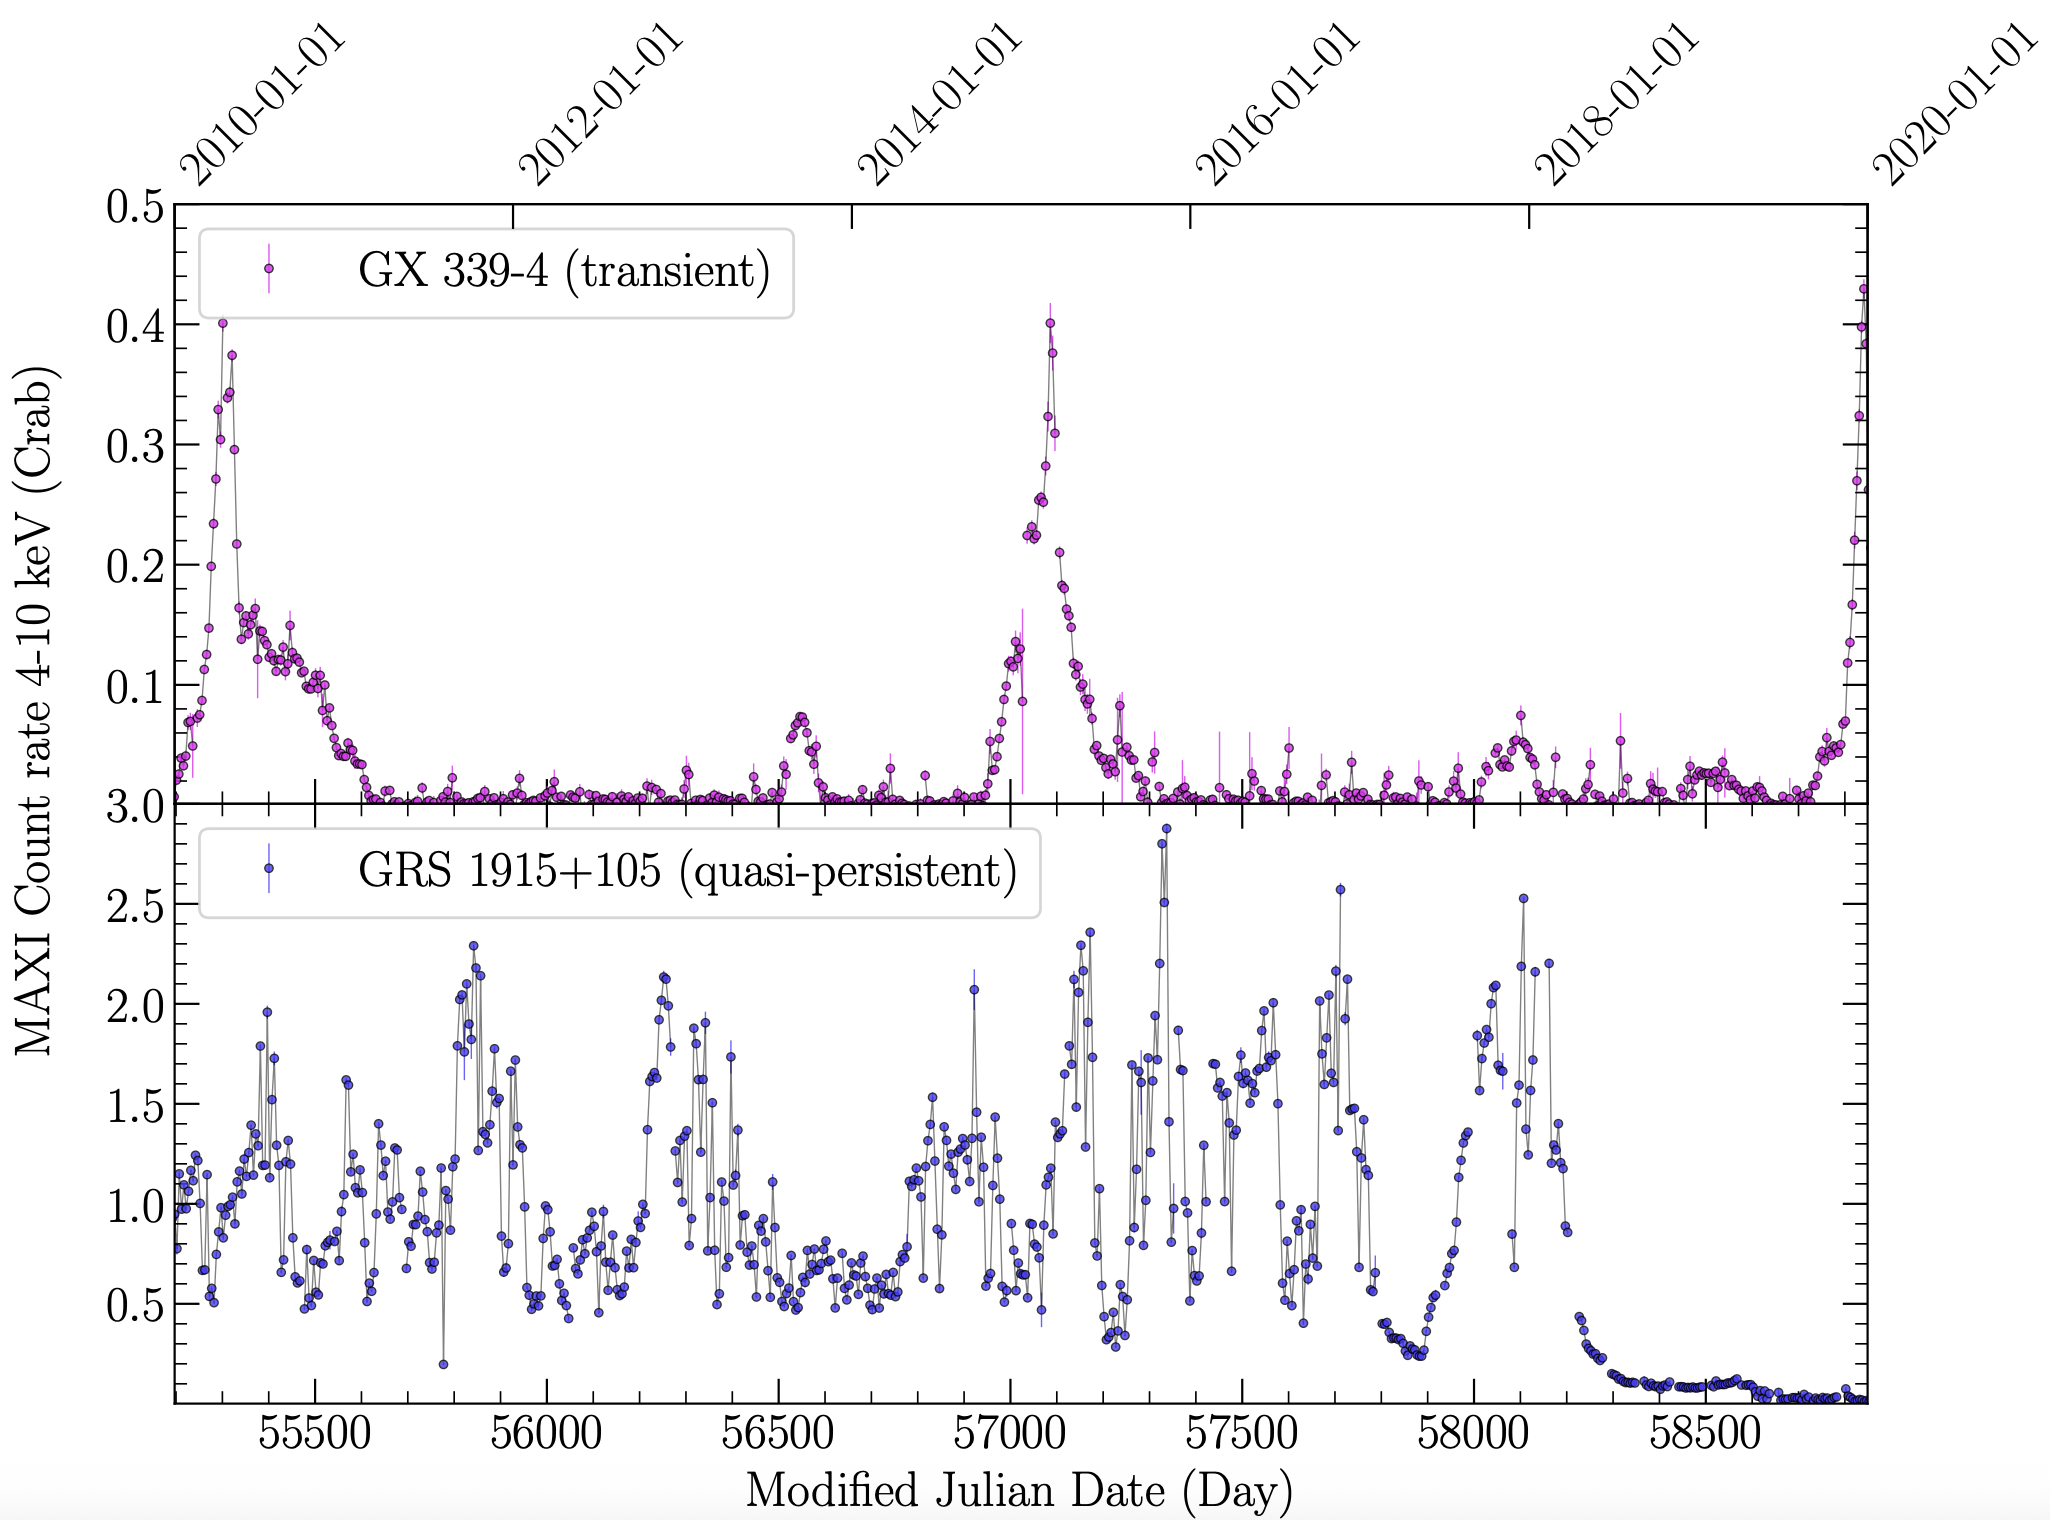
\includegraphics[width=0.75\linewidth]{Pictures/figures/lmxb_lcurves.png}
    \caption{Light curves of LMXBs and their variability over the past decade based on monitoring data from MAXI/GSC. Top: The transient black hole LMXB GX339-4, showing several distinct accretion outbursts of different brightness. Bottom: The quasi-persistent black hole LMXB GRS 1915+105, illustrating that large variations in brightness can also occur in systems that are continuously active.}
    \label{fig:placeholder}
\end{figure}
Low-Mass X-ray Binaries (LMXBs) are primarily characterized by their \textbf{phenomenological behavior}, meaning the observable changes in their emission over time. A significant population of these systems are so-called \textbf{soft X-ray transients} or \textbf{X-ray novae}. These LMXBs exhibit dramatic outbursts separated by long periods of quiescence, although other systems can display quasi-persistent X-ray emission (see Figure X).

The fundamental difference between transient and persistent behavior lies in the \textbf{stability of the accretion disk}. If the mass transfer rate from the companion star is sufficiently high, the disk remains hot and ionized, leading to stable accretion and persistent X-ray emission. However, if the rate falls below a critical threshold, the disk becomes unstable, resulting in a cycle of long quiescent phases punctuated by brief, luminous outbursts.

The \textbf{quiescent phase} is of immense astrophysical value. During this period, the accretion disk is extremely dim, allowing for unobscured observation of the companion star, which is best done in optical bands. This provides a crucial window to characterize the binary system by studying details in the star's light curve. Most importantly, we can observe the periodic \textbf{ellipsoidal variations} caused by the tidal distortion of the companion star as it orbits, which is essential for determining the system's inclination and, ultimately, the mass of the compact object.

\subsection{Spectroscopic Characteristics and States}

\begin{figure}[ht!]
    \centering
    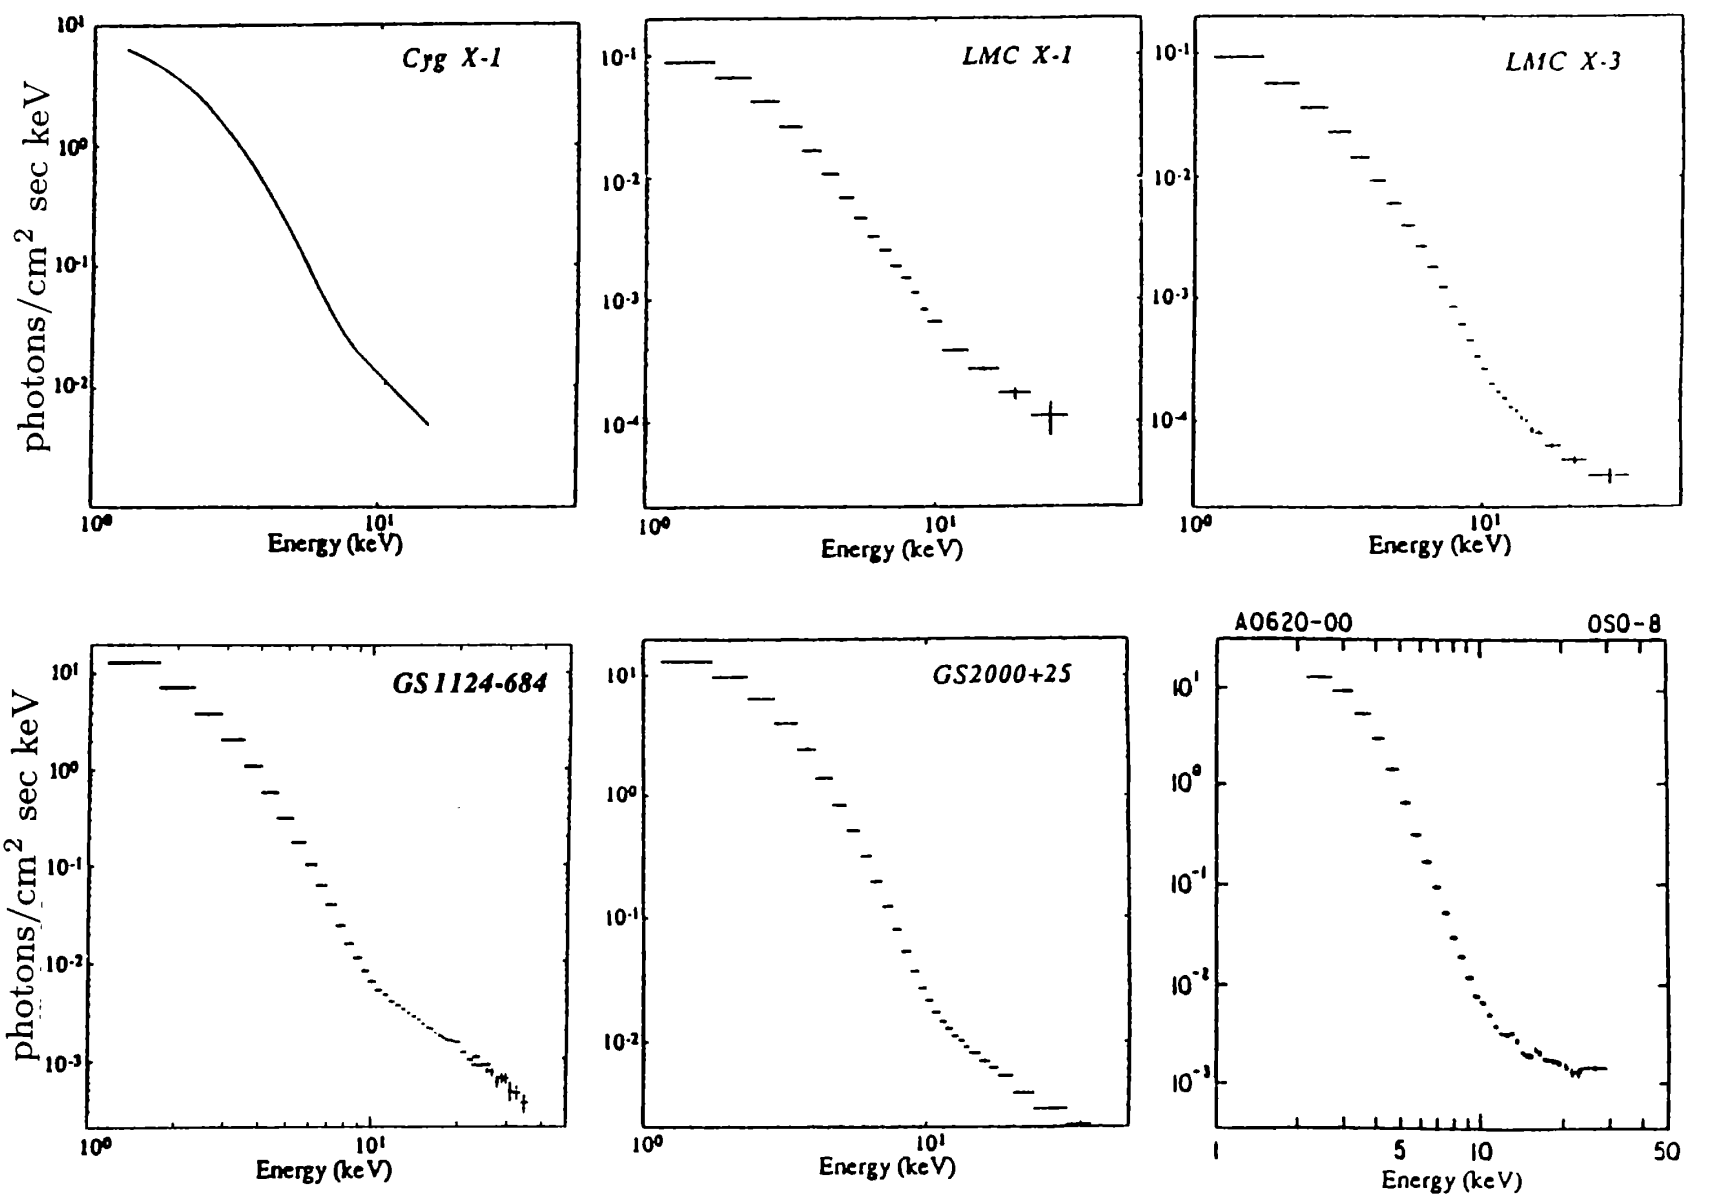
\includegraphics[width=0.75\linewidth]{Pictures/figures/lmxb_spectra.png}
\caption{A model of a typical X-ray spectrum for a Low-Mass X-ray Binary. The total observed spectrum (solid black line) is a composite of several physical components. The dominant thermal emission from the accretion disk is modeled as a \textbf{disk blackbody} (blue curve), which characterizes the bright, High/Soft State. In contrast, the \textbf{Low/Hard State} is dominated by a non-thermal power-law produced by \textbf{Comptonization} (red dashed line) in a hot corona. Additionally, hard X-rays from the corona can reflect off the surface of the accretion disk, producing a \textbf{reflection} component (green dotted line) which includes features like the relativistically broadened iron line.}
\end{figure}

The X-ray spectrum of an LMXB is not static; it provides a rich diagnostic of the accretion flow, which changes dramatically depending on the system's state. While thermal emission is a key component, the full spectrum reveals a more complex picture involving non-thermal processes and the effects of general relativity. LMXBs primarily exhibit two distinct spectral states:
\vspace{10pt}
\begin{itemize}
    \item \textbf{The High/Soft State:} During the peak of an outburst, the spectrum is dominated by strong, soft thermal emission from the accretion disk. This is not a single blackbody, but rather a \textbf{multi-temperature blackbody spectrum} arising from the temperature gradient across the disk, with the inner regions being the hottest. Fitting this thermal continuum allows astronomers to estimate the temperature and apparent inner radius of the disk, a technique which is foundational to measuring black hole spin.

    \item \textbf{The Low/Hard State:} Observed during quiescence and at the beginning and end of outbursts, this state is characterized by a much harder spectrum. The thermal emission from the disk is weak or absent. Instead, the spectrum takes the form of a \textbf{non-thermal power-law} that can extend to very high energies ($>100$ keV). This emission is understood to be the result of \textbf{Comptonization}, where soft photons are up-scattered by a corona of hot, energetic electrons surrounding the central object.
\end{itemize}
\vspace{10pt}
Beyond the continuum, LMXB spectra can display profound signatures of the extreme physics near the compact object. The most significant of these is the \textbf{relativistically broadened iron K$\alpha$ line}. While iron in the accreting gas is expected to produce a narrow emission line at 6.4 keV, the immense gravity and orbital velocity near a black hole warp its appearance. The line is smeared out by Doppler effects from the disk's rotation (approaching the speed of light) and skewed to lower energies by gravitational redshift. Modeling the precise shape of this broad iron line provides a direct probe of the innermost stable circular orbit, and is one of the primary methods used to measure the \textbf{spin of the black hole}.

\par

The journey of an LMXB through an outburst cycle is best understood as a progression through distinct accretion states, each with a unique physical geometry and a corresponding set of observational signatures. These states can be tracked using a Hardness-Intensity Diagram (HID), which maps the evolution of the X-ray spectrum and its connection to the launching of relativistic jets.
\vspace{10pt}
\begin{enumerate}

    \item \textbf{The Low/Hard State (LHS):} This is the state where the system resides during quiescence and at the beginning of an outburst.
    \begin{itemize}
        \item \textbf{Physical Nature:} The accretion flow is characterized by a cool, geometrically thin accretion disk that is truncated at a large distance from the black hole. The inner region is dominated by a hot, geometrically thick, and optically thin \textbf{corona}.
        \item \textbf{Observational Signatures:}
        \begin{itemize}
            \item \textbf{X-ray Spectrum:} The spectrum is dominated by a hard, non-thermal \textbf{power-law} produced by the Comptonization of soft photons in the hot corona. The thermal emission from the cool outer disk is very weak or absent.
            \item \textbf{Radio Emission:} A steady, compact \textbf{relativistic jet} is consistently active in this state, making the system a "microquasar."
            \item \textbf{Variability:} The X-ray emission exhibits strong, rapid, aperiodic variability (flickering) on short timescales.
            \item \textbf{Location on HID:} Occupies the right-hand branch of the HID, characterized by high hardness and low-to-medium intensity.
        \end{itemize}
    \end{itemize}

    \item \textbf{The High/Soft State (HSS):} This is the state the system transitions into near the peak of its outburst.
    \begin{itemize}
        \item \textbf{Physical Nature:} The structure of the accretion flow changes dramatically. The hot corona shrinks or disappears, and the cool, geometrically thin, and optically thick accretion disk extends all the way down to the black hole's \textbf{Innermost Stable Circular Orbit (ISCO)}.
        \item \textbf{Observational Signatures:}
        \begin{itemize}
            \item \textbf{X-ray Spectrum:} The spectrum is now dominated by soft, thermal emission. It is well-modeled as a \textbf{multi-temperature disk blackbody}, representing the combined emission from different radii of the hot inner disk.
            \item \textbf{Radio Emission:} The steady, compact jet is \textbf{quenched} or completely shut off in this state.
            \item \textbf{Variability:} The rapid X-ray variability is strongly suppressed; the emission is much more stable.
            \item \textbf{Location on HID:} Occupies the lower-left branch of the HID, characterized by low hardness and the highest intensity.
        \end{itemize}
    \end{itemize}

    \item \textbf{The Intermediate States:} These are the short-lived, complex phases that occur as the system transitions between the LHS and HSS.
    \begin{itemize}
        \item \textbf{Physical Nature:} The geometry of the accretion flow is in flux, with the inner edge of the thin disk moving inwards (during the hard-to-soft transition) or outwards (during the soft-to-hard transition).
        \item \textbf{Observational Signatures:}
        \begin{itemize}
            \item \textbf{X-ray Spectrum:} The spectrum shows a mixture of both strong thermal disk emission and a significant hard power-law tail from the Comptonizing corona.
            \item \textbf{Radio Emission:} These states are often associated with major, discrete jet ejections. As the system transitions from hard to soft, it can launch a powerful, transient blob of plasma before the steady jet fully quenches.
            \item \textbf{Location on HID:} Occupy the top, horizontal track of the HID, connecting the two main branches.
        \end{itemize}
    \end{itemize}
\end{enumerate}
\vspace{10pt}
\section{High Mass XRBs}

\begin{figure}[ht!]
    \centering
    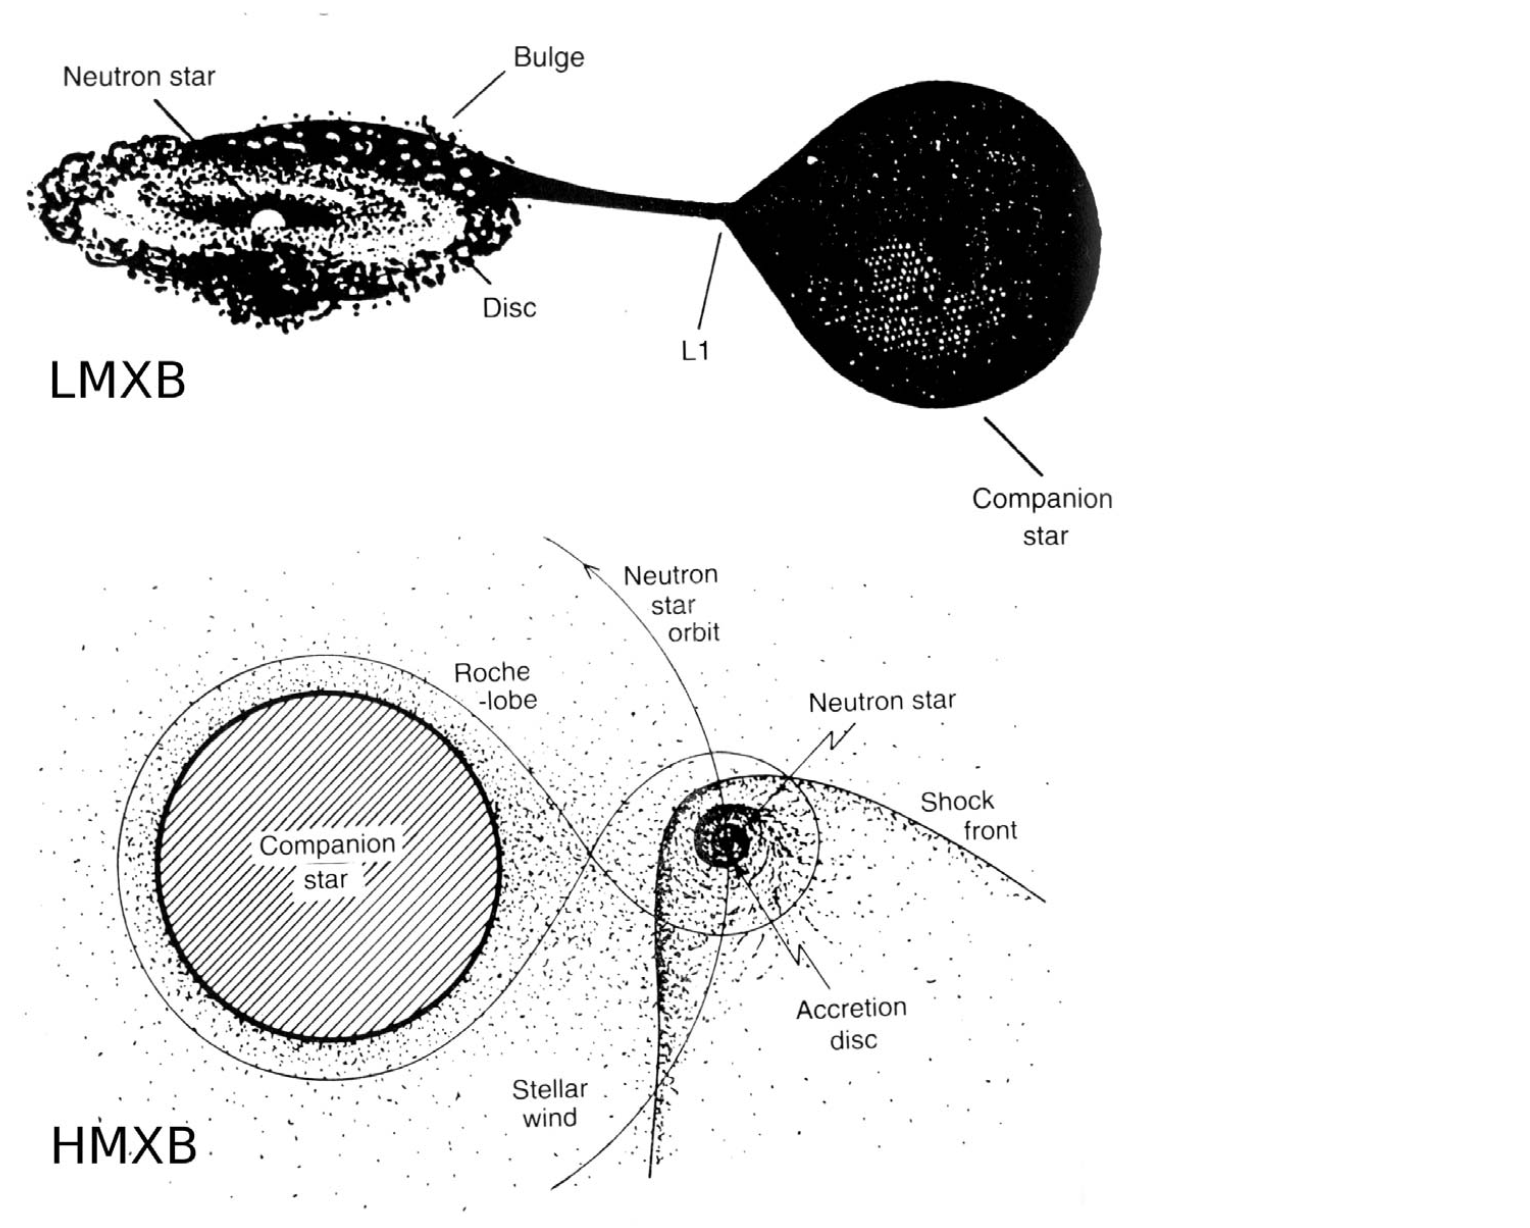
\includegraphics[width=1\linewidth]{Pictures/figures/hmxb_image.png}
    \caption{\small Artist’s conception of the two principal mechanisms by which matter is transferred onto a compact object in a binary
system. (top) A low-mass star has evolved and is losing mass to its degenerate companion because it fills its Roche lobe and mass
flows through the L 1 point. It is the presence of the compact object that distorts the mass-losing star into this shape (rather like a
pear), the vertex of which is the inner Lagrangian point, or L 1. Matter flowing out of the star forms a stream that impacts the
accretion disc (creating a bulge or thickened region) and, by viscous forces, is gradually accreted onto the compact object where
the X-rays are generated. The view is for binary phase 0.25. (bottom) The compact object is orbiting a massive star which has a
very powerful stellar wind – so powerful that there is sufficient material being lost in all directions for the compact object to
accrete and produce copious X-rays as it ploughs through this wind, thereby creating a comet-shaped shock front. The accretion
disc is small, and so fluctuations in wind density are immediately evident in the X-ray flux and pulsar frequency (courtesy EXOSAT
Observatory, ESA). (Taken from \textit{Exploring the X-ray Universe}.)}
    \label{fig:hmxb_image}
\end{figure}

High-mass X-ray binaries (HMXBs) are systems in which a compact object---typically a neutron star or a black hole---accretes material from a \textbf{massive, early-type companion star.} The donor is generally an O- or B-type star, often with masses $M_\ast \gtrsim 10\,M_\odot$, characterized by \textbf{strong stellar winds and high luminosities}. These winds provide the principal channel of mass transfer, distinguishing HMXBs from their low-mass counterparts, where \textbf{Roche-lobe overflow dominates}.

\subsection{Basic Properties}

HMXBs are among the brightest X-ray sources in the sky, with typical X-ray luminosities in the range
\[
L_X \sim 10^{35} - 10^{38}~\mathrm{erg~s^{-1}},
\]
depending on the accretion rate and compact object type. The systems generally have short orbital periods,
\[
P_{\rm orb} \sim 1~\text{to}~100~\mathrm{days},
\]
set by the balance between \textbf{wind accretion efficiency and the evolutionary state of the massive donor}.  
\begin{remark}
    It is important not to forget that the \textbf{mass-period relations} which apply to LMXBs due to the RLO mechanism are \textbf{not applicable} to wind accretion systems.
\end{remark}

The stellar wind mass-loss rate from the donor is typically
\[
\dot{M}_{\rm wind} \sim 10^{-7} - 10^{-5}\,M_\odot~\mathrm{yr^{-1}},
\]
with terminal velocities of order
\[
v_\infty \sim 1000~\mathrm{km~s^{-1}}.
\]
Only a small fraction of this wind is gravitationally captured by the compact object.\textbf{ The Bondi–Hoyle–Lyttleton accretion rate is often used as an approximation}:
\[
\dot{M}_{\rm acc} \approx \frac{(G M_{\rm X})^2 \dot{M}_{\rm wind}}
{(v_{\rm rel}^2 + c_s^2)^{3/2} a^2},
\]
where $M_{\rm X}$ is the compact object mass, $v_{\rm rel}$ is the relative velocity between the compact object and the stellar wind, $c_s$ is the sound speed in the wind, and $a$ is the orbital separation. 
The corresponding accretion luminosity is
\[
L_X \simeq \frac{G M_{\rm X} \dot{M}_{\rm acc}}{R_{\rm X}},
\]
where $R_{\rm X}$ is the radius of the compact object. For neutron stars, this yields typical luminosities near $10^{36}$--$10^{37}~\mathrm{erg~s^{-1}}$.

\subsubsection{Types of HMXBs}

High-mass X-ray binaries are broadly divided into two major subcategories based on the evolutionary state of the donor star and the dominant accretion mechanism: \textbf{supergiant systems} and \textbf{Be/X-ray binaries}. A small number of systems occupy intermediate or peculiar states, but the majority fall into one of these two classes.

\paragraph{Supergiant Systems (SGXBs)}

In \textbf{supergiant X-ray binaries} (SGXBs), the donor is an evolved O or B supergiant with a dense, radiatively driven \textbf{stellar wind}. The compact object---usually a neutron star---\textbf{accretes directly from this wind rather than through Roche-lobe overflow.} Because the accretion flow is highly inhomogeneous, these systems exhibit pronounced stochastic variability on short timescales, as well as periodic modulation with the orbital phase due to varying line-of-sight absorption.
\par
Typical parameters include:
\[
P_{\rm orb} \sim 1\text{--}10~\mathrm{days}, \quad
\dot{M}_{\rm wind} \sim 10^{-6}\,M_\odot~\mathrm{yr^{-1}}, \quad
L_X \sim 10^{36}\text{--}10^{37}~\mathrm{erg~s^{-1}}.
\]
\textbf{The X-ray luminosity is relatively steady compared to Be systems}, reflecting continuous wind capture. 
The X-ray spectrum is typically hard and highly absorbed, often displaying fluorescence features such as Fe~K$\alpha$, as well as cyclotron resonance scattering features (CRSFs) in neutron star systems, revealing the surface magnetic field strength ($B \sim 10^{12}$~G).  
\par
Some SGXBs are also \textbf{eclipsing binaries}, enabling precise dynamical mass measurements (e.g., Vela~X-1, 4U~1700$-$37, and Cyg~X-1). Others, termed \emph{supergiant fast X-ray transients (SFXTs)}, display sporadic outbursts \textbf{likely triggered by the capture of dense clumps within the stellar wind,} leading to rapid X-ray flares lasting hours to days.

\paragraph{Be/X-ray Binaries (BeXBs)}
In contrast, \textbf{Be/X-ray binaries} consist of a neutron star orbiting a rapidly rotating B-type star that possesses an equatorial \textbf{decretion disk} of gas ejected by the star’s high rotational velocity. The compact object follows a wide and often eccentric orbit ($P_{\rm orb} \sim 10$--$300~\mathrm{days}$), accreting only when it passes near periastron and interacts with the Be star’s disk. 
\par
As a result, BeXBs are typically \textbf{transient systems}, exhibiting two classes of outbursts:
\begin{itemize}
    \item \textbf{Type~I outbursts:} Regular, moderate-luminosity ($L_X \sim 10^{36}~\mathrm{erg~s^{-1}}$) events near periastron passage.
    \item \textbf{Type~II outbursts:} Giant, irregular events ($L_X \gtrsim 10^{37}~\mathrm{erg~s^{-1}}$) caused by large-scale disruptions or expansions of the Be decretion disk.
\end{itemize}

The optical spectra of Be donors are \textbf{characterized by strong Balmer emission lines (particularly H$\alpha$), arising from the circumstellar disk.} The double-peaked line profiles reflect Keplerian rotation in the disk and often vary with time as the disk grows or dissipates. These emission features both diagnose the disk dynamics and complicate radial velocity measurements.
\par
Most BeXBs host \textbf{X-ray pulsars}, where the neutron star’s strong magnetic field channels accreting material onto magnetic poles, producing pulsations with spin periods $P_{\rm spin} \sim 1$--$1000$~s. The systems show a broad correlation between orbital and spin period (the ``Corbet diagram''), reflecting the balance between wind torque and magnetospheric accretion.

\paragraph{Other and Transitional Systems}

A few systems exhibit hybrid characteristics or represent later evolutionary stages:
\begin{itemize}
    \item \textbf{Roche-lobe overflow HMXBs:} Very rare, short-period systems in which the massive donor fills its Roche lobe and drives persistent disk accretion (e.g., LMC~X-4).
    \item \textbf{Wolf–Rayet binaries:} Extremely evolved donors with powerful, helium-rich winds feeding a compact companion (e.g., Cyg~X-3).
\end{itemize}

\par
In summary, HMXB subtypes trace different stages of massive binary evolution and reveal distinct accretion physics. SGXBs probe quasi-spherical wind accretion and radiative feedback, while BeXBs highlight transient disk-fed accretion and magnetically channeled flows. Together, they form the dominant population of X-ray binaries in young stellar environments and provide essential constraints on compact object formation and binary evolution pathways.

\subsubsection{Localization of HMXBs}

High-mass X-ray binaries are found \textbf{predominantly in regions of active or recent star formation}, reflecting the short lifetimes of their massive stellar companions. Since O- and B-type stars evolve on timescales of only a few million years, HMXBs trace the \emph{young stellar population} of a galaxy. Their spatial distribution therefore offers strong evidence that they are short-lived evolutionary phases in the lives of massive binaries.

\par
Within the Milky Way, HMXBs are concentrated along the Galactic plane and particularly near the spiral arms, coinciding with sites of ongoing star formation such as OB associations and H\,\textsc{ii} regions. This localization is consistent with the fact that their progenitor binaries form and evolve rapidly before the massive star undergoes core collapse. The compact object (a neutron star or black hole) forms in a supernova, and if the binary survives the explosion, it remains close to its birthplace.
\par
Because of these youth and kinematic properties:
\begin{itemize}
    \item HMXBs are often located within a few hundred parsecs of star-forming complexes or molecular clouds.
    \item They exhibit moderate space velocities ($\sim 10$--$100~\mathrm{km~s^{-1}}$), potentially imparted by the supernova kick, but not sufficient to carry them far from their birth sites.
    \item Their vertical scale height above the Galactic plane is small ($z \lesssim 200$~pc), consistent with Population~I objects.
\end{itemize}
\par
In contrast, \textbf{low-mass X-ray binaries (LMXBs)} show a completely different spatial distribution. Their old, low-mass donors imply long evolutionary timescales, allowing them to migrate far from their birthplaces. Consequently, LMXBs are found throughout the Galactic bulge and halo, and many are associated with \textbf{globular clusters}. Their high scale heights ($z \sim 1$--$2$~kpc) reflect their membership in the old stellar population.
\par
The differing localizations of HMXBs and LMXBs therefore trace the star-formation history of galaxies: 
HMXBs mark \textbf{young, massive stellar environments}, while LMXBs trace the \textbf{ancient, dynamically evolved populations}. In external galaxies, this distinction manifests as a strong correlation between HMXB number and recent star-formation rate, and between LMXB number and total stellar mass.

\subsubsection{Accretion Mechanisms}

In high-mass X-ray binaries, accretion proceeds primarily through the capture of the \textbf{stellar wind} from the massive companion. The strong, radiatively driven wind of an O/B supergiant provides a continuous outflow of material that the compact object can gravitationally capture. This process is well described by the \textbf{Bondi–Hoyle–Lyttleton (BHL) accretion model}, in which the compact object effectively sweeps up a fraction of the stellar wind as it moves through it.

\par
The mass accretion rate is approximately
\[
\dot{M}_{\rm acc} \approx \pi R_{\rm acc}^2 \rho v_{\rm rel},
\qquad
R_{\rm acc} = \frac{2 G M_{\rm X}}{v_{\rm rel}^2 + c_s^2},
\]
where $R_{\rm acc}$ is the accretion radius, $\rho$ is the local wind density, $v_{\rm rel}$ is the relative velocity between the compact object and the wind, and $c_s$ is the sound speed. Only a small portion of the stellar wind is accreted, but given the high wind mass-loss rates, this is sufficient to generate X-ray luminosities of $L_X \sim 10^{36}$--$10^{37}~\mathrm{erg~s^{-1}}$.

\par
As the accreted material approaches the compact object, it encounters the \textbf{magnetosphere} of the neutron star. At the \textbf{magnetospheric radius} $R_{\rm m}$, the magnetic pressure balances the ram pressure of the inflowing gas. Inside this radius, the magnetic field dominates the flow dynamics, forcing the plasma to follow magnetic field lines and funneling it toward the magnetic poles. 

\par
At the neutron star surface, the inflow decelerates in a strong shock, forming a localized \textbf{accretion column} where kinetic energy is converted into thermal and radiative energy. The resulting hot spots emit primarily in X-rays, with characteristic luminosities up to $\sim 10^{38}~\mathrm{erg~s^{-1}}$. If the magnetic axis is \textbf{misaligned with the rotation axis}, the emission appears modulated at the stellar spin period, producing the characteristic \textbf{X-ray pulsar} phenomenon. These pulsations directly probe the rotation rate, magnetic field structure, and accretion geometry of the compact object.

\par
In contrast, \textbf{Be/X-ray binaries} operate through a different, highly variable accretion mode. The Be donor possesses a dense, equatorial \textbf{decretion disk} of gas expelled by rapid rotation. The compact object, typically in an eccentric orbit, captures material from this disk primarily during periastron passages. The interaction triggers episodic accretion events and consequent X-ray outbursts. 

\par
Two types of outbursts are typically observed:
\begin{itemize}
    \item \textbf{Type~I outbursts:} Modest, periodic events ($L_X \sim 10^{36}~\mathrm{erg~s^{-1}}$) occurring near periastron.
    \item \textbf{Type~II outbursts:} Bright, irregular outbursts ($L_X \gtrsim 10^{37}~\mathrm{erg~s^{-1}}$), associated with large-scale expansions or instabilities in the Be disk.
\end{itemize}

\par
In both wind-fed and Be-fed systems, the details of accretion---including angular momentum capture, magnetic coupling, and radiative feedback---play key roles in setting the X-ray luminosity and variability. Together, these mechanisms underpin the rich phenomenology of HMXBs, linking stellar winds, magnetospheric physics, and high-energy radiation in a unified framework.

\subsection{HMXBs as Spectroscopic Binaries}

Since the O/B-type companion in a high-mass X-ray binary is extremely \textbf{luminous}, we can generally observe both the emission from the accretion process (\textbf{X-ray radiation}) and the emission from the massive companion (\textbf{optical/UV continuum}). This dual visibility makes HMXBs \textbf{double-lined spectroscopic binaries}, allowing dynamical studies of both components and, consequently, direct constraints on the compact object mass.

\par
The donor star’s spectrum is dominated by its photospheric absorption lines (H~I, He~I, He~II, and various metallic features). However, the presence of the compact object and its energetic radiation field substantially alters the observed optical spectrum. X-ray photoionization of the stellar wind and reprocessing in the accretion flow introduce strong \textbf{emission components}---particularly in the Balmer series (most notably H$\alpha$), He~II~$\lambda4686$, and sometimes Fe~II and N~III lines. These can \textbf{partially fill in} or even \textbf{reverse} the absorption features, leading to distorted or asymmetric line profiles. The resulting composite spectrum often varies with orbital phase, reflecting changes in the ionization structure of the stellar wind and accretion wake. Even in the optical, this can produce a veiling of the photospheric lines, complicating radial velocity measurements and spectral classification.

\par
In systems hosting neutron stars, \textbf{X-ray pulsations} provide a direct tracer of the compact object’s orbital motion. In others, Doppler shifts in X-ray or emission-line features from the accretion flow can be used to extract the compact object’s velocity amplitude $K_{\rm X}$. Meanwhile, the O/B star’s optical spectrum traces its own motion with velocity amplitude $K_\ast \sim 10$--$100~\mathrm{km~s^{-1}}$. The ratio of these amplitudes yields the binary mass ratio:
\[
\frac{M_{\rm X}}{M_\ast} = \frac{K_\ast}{K_{\rm X}}.
\]
Combining this ratio with the orbital period $P_{\rm orb}$ provides the \textbf{standard mass function,}
\[
f(M) = \frac{(M_{\rm X} \sin i)^3}{(M_\ast + M_{\rm X})^2}
= \frac{P_{\rm orb} K_\ast^3}{2\pi G},
\]
which sets a firm \emph{lower bound} on the \textbf{mass of the compact object.} For eclipsing systems, where the inclination $i$ can be accurately determined ($i \gtrsim 75^\circ$), both $M_{\rm X}$ and $M_\ast$ can be measured directly with relatively small uncertainties.

\par
Spectroscopic complications are especially pronounced in supergiant systems, where dense winds and strong X-ray irradiation produce extended emission-line regions, and in Be/X-ray binaries, where the Be star’s decretion disk gives rise to variable, double-peaked Balmer emission lines. These effects must be carefully modeled to disentangle stellar, disk, and wind contributions. Nonetheless, the ability to observe both components spectroscopically makes HMXBs among the most powerful laboratories for constraining compact object masses and testing models of binary evolution.

\subsection{Observational Diagnostics}

High-mass X-ray binaries display a wide range of \textbf{observational signatures} that reveal the complex interplay between accretion, radiation, and stellar winds. Their variability spans timescales from seconds to years and offers a powerful window into the geometry and dynamics of the accretion process. 

\par
A defining feature of HMXBs is their \textbf{orbital modulation} of X-ray flux. As the compact object traverses the dense stellar wind of its massive companion, the line-of-sight column density varies periodically, leading to strong changes in observed brightness. In many systems, this modulation is further enhanced by geometric \textbf{eclipses}, during which the donor star partially or completely obscures the X-ray source. Because the absorbing material contains metals, the increased column density preferentially extinguishes soft X-rays, producing phase-dependent changes in the continuum shape. Even in deeply eclipsing systems, however, \textbf{radiative transfer and photoionization} within the wind ensure that emission lines remain visible, as they originate from extended regions of ionized gas rather than from the compact source itself.

\par
Another characteristic signature arises from \textbf{X-ray pulsations}, observed in systems hosting magnetized neutron stars. In these binaries, the accreting material is funneled along magnetic field lines onto the neutron star’s magnetic poles, forming localized hot spots. As the neutron star rotates, the anisotropic emission from these poles produces coherent pulsations, with periods ranging from $\sim 1$ to $1000$~s. The pulse profiles and their energy dependence provide valuable constraints on the geometry of the accretion column and the strength and configuration of the magnetic field.

\par
In addition to these periodic signals, HMXBs exhibit a rich variety of \textbf{long-term and aperiodic variability}. Changes in the density and structure of the stellar wind can modulate the accretion rate on timescales of weeks to months, while in Be/X-ray binaries, the quasi-cyclic formation and dissipation of the Be star’s decretion disk drive recurring outbursts and extended quiescent phases. Some systems show distinct \textbf{spectral state changes}, transitioning between high- and low-luminosity states that are often accompanied by variations in hardness ratio. These transitions typically trace fluctuations in the accretion rate or shifts in the absorbing column along the line of sight.

\par
Spectroscopically, HMXBs display \textbf{complex and diagnostic X-ray spectra} that encode the physical properties of the accretion environment. The continuum emission is generally hard, arising from \textbf{thermal bremsstrahlung} or \textbf{Comptonized emission} within the accretion column or corona. Superimposed on this continuum are strong spectral features, most notably the \textbf{Fe~K$\alpha$ fluorescence line} at 6.4~keV, which originates from reprocessing in cool, dense material near the compact object. Additional photoionization and recombination lines reveal the presence of extended, partially ionized gas in the stellar wind. Many systems also exhibit \textbf{energy-dependent absorption}, with partial-covering models required to explain spectra affected by dense or clumpy winds. These absorption effects frequently produce sharp low-energy cutoffs and variable attenuation of the continuum flux.

\par
Taken together, these timing and spectral diagnostics make HMXBs uniquely valuable laboratories for studying accretion under extreme conditions. They provide empirical constraints on wind-fed accretion, magnetic channeling, and radiative feedback, linking the physics of massive stars to the high-energy behavior of compact objects in binary systems.



\subsection{Spectroscopic Features}

The composite spectra of high-mass X-ray binaries reflect contributions from both the massive donor star and the compact accretor, as well as their mutual interaction through winds and radiation. Each component imprints distinct features across the electromagnetic spectrum.

\subsubsection{Stellar and Wind Signatures}

The \textbf{optical and UV spectra} are dominated by the massive O/B-type donor, which exhibits strong photospheric absorption lines (H~I, He~I, He~II, and various metal lines). However, X-ray irradiation and the presence of a dense, structured stellar wind significantly modify these features:
\begin{itemize}
    \item Reprocessing in the wind produces prominent \textbf{emission lines}, particularly H$\alpha$, He~II~$\lambda4686$, and Fe~II multiplets, which can partially fill in or even reverse absorption features.
    \item The stellar wind is highly \textbf{clumpy and anisotropic}, giving rise to stochastic variability and asymmetric line profiles that vary with orbital phase. This was found by \citet{1999ApJ...525..921S} based on the presence of spectroscopic signatures from both cold gas and photoionized gas suggesting inhomogeneity.
    \item In Be/X-ray binaries, the decretion disk adds strong, often double-peaked Balmer emission lines tracing Keplerian rotation in the disk.
\end{itemize}

\subsubsection{X-ray Spectral Features}

The \textbf{X-ray emission} arises primarily from hot, shocked plasma near the compact object. The continuum is typically a power law with an exponential cutoff above $\sim 10$--$30$~keV, consistent with \textbf{thermal bremsstrahlung} or \textbf{Comptonized emission} from the accretion column or corona. Superimposed on this continuum are:
\begin{itemize}
    \item \textbf{Emission lines} from highly ionized species (e.g., Fe~XXV, Fe~XXVI), produced by photoionization in the stellar wind.
    \item The ubiquitous \textbf{Fe~K$\alpha$ fluorescence line} at 6.4~keV, a key tracer of dense, neutral material near the compact object.
    \item Broad absorption features identified as \textbf{cyclotron resonance scattering features (CRSFs)}, which directly measure the magnetic field strength of the neutron star.
    \item Variable absorption edges and partial covering components, reflecting the inhomogeneous wind and orbital modulation of the column density.
\end{itemize}

\subsubsection{Eclipsing and Reprocessing Effects}

In \textbf{eclipsing HMXBs}, the optical star can completely block the direct continuum X-ray emission when the compact object passes behind it. During such eclipses, the observed spectrum becomes dominated by \textbf{scattered and reprocessed emission} originating in the extended stellar wind and circumstellar gas. Remarkably, while the continuum flux drops dramatically, the emission lines remain largely unchanged, since they are produced in photoionized gas on scales much larger than the stellar radius.

\par
This behavior allows observers to isolate the reprocessed emission and study the ionization structure and density of the surrounding medium, providing a natural laboratory for testing radiative transfer and wind models in high-energy astrophysical environments.


\subsection{Evolution of HMXBs}
\begin{figure}
    \centering
    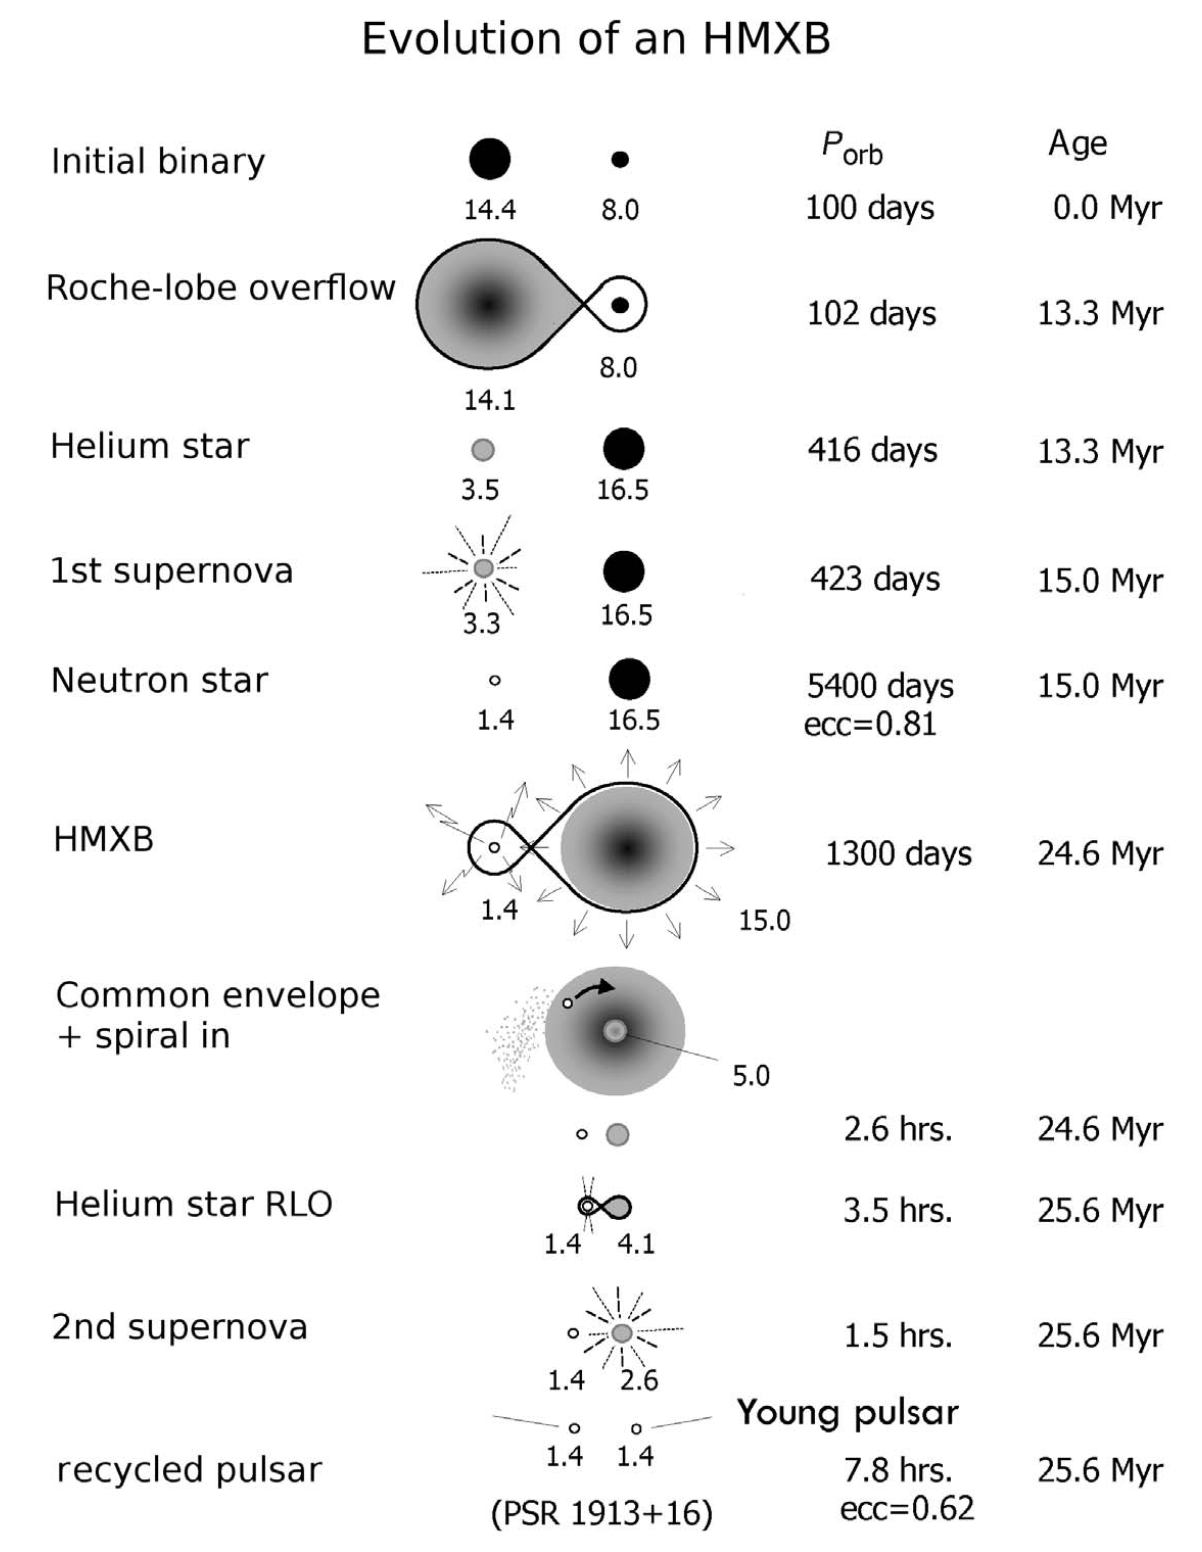
\includegraphics[width=1\linewidth]{Pictures/figures/hmxb_evol.png}
    \caption{Evolutionary scenario for the formation of an HMXB/Be star from an initial binary of two stars of differing large mass
at age 0. The more massive star evolves fastest, producing the first supernova event after 15 Myr. The resulting neutron star leads
to the HMXB/Be phase once the surviving star has itself evolved to become a giant. This phase does not last long, and following a
common-envelope ‘spiral-in’, a second supernova event can lead to the formation of a binary pulsar system (diagram based on
Tauris \& van den Heuvel, 2006). (Taken from \textit{Exploring the X-ray Universe}.)}
    \label{fig:hmxb_evolution}
\end{figure}
The canonical formation path for a high-mass X-ray binary proceeds through a sequence of short-lived but observationally supported stages. A representative example begins with a massive binary (orbital period $\sim$100~days) in which the initially \emph{more massive} primary evolves rapidly, expands, and fills its Roche lobe after $\sim 13$~Myr, initiating the \textbf{first mass-transfer episode}. In the illustrative case shown, $\sim 9\,M_\odot$ are transferred to the companion in $\sim 5\times10^4$~yr, leaving a $\sim 3.5\,M_\odot$ helium core and widening the orbit to $\gtrsim 400$~days due to mass and angular-momentum exchange.
\rmk{Remember, we are transferring from the more massive primary to the less massive secondary, which means the orbit will expand.}
\paragraph{Helium-star (Wolf–Rayet) phase and the first supernova.}
After envelope stripping, the primary is observed as a helium (Wolf–Rayet) star whose energy source is helium fusion; within $\sim 2$~Myr it undergoes \emph{the first core-collapse supernova}. The prompt mass loss and explosion asymmetry typically yield a highly eccentric, longer-period post-SN orbit—and often disrupt the binary entirely, a fact that helps explain the rarity of X-ray binaries.

\paragraph{The HMXB phase.}
If the binary survives, the compact remnant (usually a neutron star) orbits the still-massive secondary. While that secondary remains an O/B star, wind-fed accretion powers the \emph{HMXB} episode; \textbf{this phase is comparatively brief in population terms}. As the donor later evolves and \emph{expands}, mass transfer becomes dynamically unstable (for extreme mass ratios, $q\!=\!M_{\rm donor}/M_{\rm acc}\!\gg\!1$), leading to \emph{common-envelope (CE) evolution}: friction in the shared envelope removes orbital energy and angular momentum, driving a spiral-in. The outcome is a dramatic period shrinkage to hours and ejection of the donor’s H-rich envelope, leaving a tight neutron-star + helium-star system. For context on stability: Roche-lobe overflow is \emph{only} stably maintained when the donor is \emph{less} massive than the accretor; when the donor is more massive (as in this stage) instability and CE are expected.

\paragraph{Roche-lobe overflow from the helium star and the second supernova.}
In the post-CE binary, the stripped helium star can subsequently \emph{overflow its Roche lobe} and transfer mass onto the neutron star in a short-period orbit, before ultimately undergoing a \emph{second} supernova. A surviving system emerges as a \emph{double neutron star}—as exemplified by radio pulsar binaries such as PSR~1913+16—providing striking observational evidence for this evolutionary channel. 

\paragraph{Link to star-formation history.}
Because HMXB lifetimes are short, their numbers and luminosity functions \emph{track recent star formation}. The pronounced overabundance of HMXBs in the SMC is explained by a $\sim 100$~Myr-old interaction-triggered starburst, and across external galaxies the cumulative HMXB luminosity functions align when scaled by the star-formation rate, making HMXBs effective SFR indicators.

\subsection{Relativistic Jets}
- The blue jet and the optical jet are not quite the same. Unclear why? 
- The relativistic jets and the kinetic view of them -> how we use SR to get the velocities due to transverse doppler shift.

\section{The Nature of the Accretor}

\begin{figure}[ht!]
    \centering
    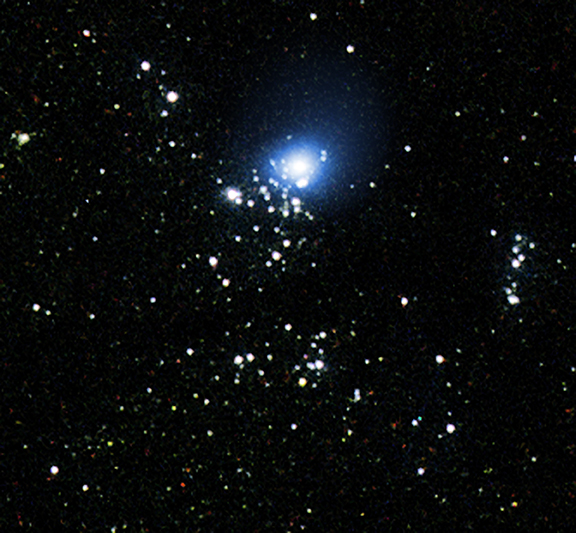
\includegraphics[width=0.5\linewidth]{Pictures/figures/x-7.png}
    \caption{The composite image includes data from NASA's Chandra X-ray Observatory (blue) and the Hubble Space Telescope. The bright objects in the inset image are young, massive stars around M33 X-7, and the bright, blue Chandra source is M33 X-7 itself. X-rays from Chandra reveals how long the black hole is eclipsed by the companion star, which indicates the size of the companion. }
\end{figure}

Once an X-ray binary is identified, a fundamental question arises: is the compact object accreting matter a neutron star or a black hole? Since black holes emit no light themselves, their presence must be inferred gravitationally. The definitive discriminant is mass. Theory and observation place a firm upper limit on the mass of a stable neutron star, known as the Tolman-Oppenheimer-Volkoff limit, at approximately $3 M_{\odot}$. Any compact object with a dynamically measured mass that conclusively exceeds this threshold cannot be a neutron star and is therefore considered a black hole.

Low-Mass X-ray Binaries (LMXBs) have proven to be the most fertile ground for finding and weighing stellar-mass black holes. The low mass of the companion star means that any measurement of the system's total mass is dominated by the compact object, providing a cleaner result. Crucially, the long quiescent periods of transient LMXBs are a gift to observers; with the accretion disk dormant and faint, the light from the faint companion star can be isolated and studied in detail to precisely measure its orbital parameters.

The primary tool for this task is the \textbf{mass function}, derived from observing the spectral lines of the visible companion star in what is known as a single-lined spectroscopic binary. By measuring the star's orbital period ($P$) and the amplitude of its radial velocity ($K_c$), one can calculate the mass function, $f(M)$:

\[
f(M) = \frac{P K_c^3}{2\pi G} = \frac{(M_X \sin i)^3}{(M_X + M_c)^2}
\]

where $M_X$ and $M_c$ are the masses of the compact object and companion, respectively, and $i$ is the orbital inclination. The value $f(M)$ provides an absolute minimum mass for the compact object ($f(M) \leq M_X$). Several LMXBs have mass functions well in excess of $3 M_{\odot}$, providing unambiguous proof of a black hole.

While LMXBs are ideal, the most "gold-standard" confirmations can come from rare systems with special geometries. A prime example is \textbf{M33 X-7}, a High-Mass X-ray Binary that happens to be an \textbf{eclipsing} system. The presence of deep eclipses tells us that we are viewing the orbit almost perfectly edge-on ($i \approx 90^{\circ}$), which eliminates the main uncertainty in the mass function since $\sin i \approx 1$. With the inclination constrained, the mass of the accretor was precisely measured to be $15.65 \pm 1.45 M_{\odot}$. This value is more than five times the maximum possible mass of a neutron star, making M33 X-7 one of the most securely identified black holes known.
\chapter{Tidal Disruption Events}
A \textbf{tidal disruption event} occurs in scenarios where a star's orbit brings it within a close enough radius of a black hole to disrupt the star. The material from the star may then be either partially accreted or fully accreted in a luminous transient event. In this section, we'll discuss the theory and relevant observational context of these events.

\section{TDE Theory}
Before we dig into the observational details of TDEs, we'll first discuss the theory of TDE formation and the relevant scalings and typical equations in play. 

\subsection{Tidal Disruption}

Tidal forces on a star of radius $R_\star$ and mass $M_\star$ become relevant only when their corresponding gravitational field \textbf{varies significantly from one side of the star to the other}. Assuming that the star is originally at radius $r$ from the point mass it is orbiting, the star will then rest in the potential
\[
\Phi = -\frac{GM}{r}.
\]
In such a potential, the center of mass of the star moves in an orbit as described by standard mechanics. The relative force $dF_i$ in direction $x^i$ due to a shift in position $dx^j$ is 
\[
dF_i = \nabla_i \Phi(x + dx^j),
\]
which defines a \emph{tidal tensor} that characterizes the second derivatives of the gravitational potential.
\vspace{10pt}
\begin{definition}[Tidal Tensor]
The \textbf{tidal tensor} describes the differential gravitational acceleration across a finite-sized body in an external potential. It is given by
\begin{equation}
    \label{eq:tidal_tensor}
    \boxed{
    T_{ij} = -\Phi_{;ij} = \frac{\partial^2 \Phi}{\partial x^i\partial x^j}.
    }
\end{equation}
The corresponding \textbf{differential force} due to a shift $\delta {\bf x}$ is 
\[
\delta {\bf F} = \bf{T} \delta {\bf x}.
\]
\par
For a point-mass potential $\Phi = -GM/r$, this becomes
\[
T_{ij} = \frac{GM}{r^3}\left(3 - \delta_{ij}\right).
\]
The eigenvalues of $T_{ij}$ quantify the degree of stretching or compression along different directions in space.
\end{definition}
\vspace{10pt}
If the differential tidal acceleration across the star \textbf{exceeds its own self-gravity}, the star can no longer maintain hydrostatic equilibrium and is torn apart. At the surface of a star of radius $R_\star$, the tidal tensor tells us that the differential force is
\[
{\bf F}_{\rm tidal} = {\bf F}(r + R_\star) - {\bf F}(r) 
\simeq \left(\frac{d{\bf F}}{dr}\right) R_\star
= \left(\frac{GM}{r^3}\right) R_\star,
\]
which corresponds to a differential acceleration
\[
a_{\rm tidal} \sim \frac{GM R_\star}{r^3}.
\]
This is the characteristic acceleration difference felt between the near and far sides of the star due to the black hole’s gravitational field.

The star’s own self-gravity at its surface, which provides the restoring acceleration maintaining hydrostatic balance, is
\[
a_{\rm self} \sim \frac{G M_\star}{R_\star^2}.
\]
When $a_{\rm tidal} \gtrsim a_{\rm self}$, the black hole’s tidal forces dominate over the star’s self-gravity, and the star is disrupted. Setting the two equal defines the \textbf{tidal radius} $r_t$:
\[
\frac{G M R_\star}{r_t^3} = \frac{G M_\star}{R_\star^2}
\quad \Longrightarrow \quad
\boxed{r_t = R_\star \left(\frac{M}{M_\star}\right)^{1/3}}.
\]
This simple scaling captures the essential physics: \textbf{more massive black holes have larger tidal spheres of influence}, while more compact (smaller $R_\star$) or massive ($M_\star$) stars are harder to disrupt. In practice, the exact disruption condition depends on the internal structure of the star, the encounter geometry, and relativistic corrections for very massive black holes.
\par
It is worth looking at this scaling in a fiducial context. For stars of approximately solar mass and radius and black holes of mass around $10^6\;{\rm M_\odot}$, the relationship
\[
\begin{aligned}
    r_t &\approx 7 \times 10^{12} \left(\frac{R_\star}{R_\odot}\right) \left(\frac{M}{10^6\;{\rm M_\odot}}\right)^{1/3} \left(\frac{M_\star}{M_\odot}\right)^{-1/3} \; {\rm cm}\\
    &\approx 0.5 \left(\frac{R_\star}{R_\odot}\right) \left(\frac{M}{10^6\;{\rm M_\odot}}\right)^{1/3} \left(\frac{M_\star}{M_\odot}\right)^{-1/3} \; {\rm AU}
\end{aligned}
\]
\par
Another feature of these systems which is worth being aware of is the $r_t$ is \textbf{not always outside the event horizon}. For a Schwarzchild black hole, 
\[
r_s = \frac{2GM}{c^2} \implies \frac{r_t}{r_s} =\frac{c^2}{2G}\; R_\star M_\star^{-1/3} M^{-2/3}.
\]
For relevant scalings,
\[
\frac{r_t}{r_s} \approx 5 \left(\frac{R_\star}{R_\odot}\right) \left(\frac{M_\star}{M_\odot}\right)^{-1/3}\left(\frac{M}{10^7\;{\rm M_\odot}}\right)^{-2/3}.
\]
And so for black holes larger than about $10^7$, tidal disruption simply cannot occur.
\par
If the \textbf{pericenter} of the stellar orbit passes within $r_t$ of the black hole, then disruption will occur. The degree of disruption depends sensitively on the ratio $\beta \equiv r_t / r_p$, known as the \textbf{penetration factor}. For $\beta \lesssim 1$, the star \textbf{may only be partially stripped}, losing a small fraction of its envelope. For $\beta \gtrsim 1$, the \textbf{star is fully disrupted}, and its material is stretched into a long, thin stream by tidal forces.

\subsection{Accretion onto the Black Hole}

Assuming the \textbf{ballistic approximation}, the star is completely torn apart as it crosses the tidal radius $r_t$, and the stellar debris moves thereafter in the gravitational field of the black hole \textbf{without significant hydrodynamic interaction}. Each fluid element inherits approximately the velocity of the stellar center of mass at the moment of disruption but originates from a slightly different position within the star. This positional offset \textbf{leads to a spread in the specific orbital energy of the debris.}

The specific orbital energy of a test particle in the gravitational potential of the black hole is
\[
\epsilon = \frac{1}{2}v^2 - \frac{GM}{R}.
\]
Expanding about the tidal radius $r_t$, we find that the differential in energy across the stellar diameter is approximately
\[
\Delta \epsilon \approx \left.\frac{d\Phi}{dr}\right|_{r_t} R_\star = \frac{GM}{r_t^2} R_\star = \epsilon_\star \left(\frac{M}{M_\star}\right)^{1/3},
\]
where $\epsilon_\star = GM_\star / R_\star$ is the characteristic binding energy per unit mass of the star. Thus, the debris inherits a roughly uniform distribution of energies between
\[
-\Delta \epsilon \leq \epsilon \leq +\Delta \epsilon.
\]

Because the original stellar orbit is nearly parabolic ($\epsilon \approx 0$), half of the debris ends up with $\epsilon < 0$ and remains gravitationally bound to the black hole, while the other half with $\epsilon > 0$ becomes unbound and escapes on hyperbolic trajectories. \textbf{Importantly, both bound and unbound debris streams \emph{initially pass through the same pericenter} $r_p \approx r_t$}, because they are all launched from approximately the same point in space at the moment of disruption. What differs between them is their \emph{orbital energy}, and hence their semimajor axis and eccentricity.

\paragraph{Eccentricities of the Bound Debris.}
For the bound material, the semimajor axis of a given debris element is related to its specific energy by
\[
a = -\frac{GM}{2\epsilon}.
\]
Since the most tightly bound debris has $\epsilon = -\Delta \epsilon$, its semimajor axis is
\[
a_{\rm min} = \frac{GM}{2\Delta \epsilon} \approx \frac{r_t^2}{2R_\star} \approx \frac{1}{2}R_\star \left(\frac{M}{M_\star}\right)^{2/3}.
\]
The corresponding orbital eccentricity is determined by the relation between pericenter and semimajor axis:
\[
e = 1 - \frac{r_p}{a}.
\]
Substituting $r_p \approx r_t$ and $a = a_{\rm min}$ gives
\[
e_{\rm min} = 1 - 2\frac{R_\star}{r_t}
\simeq 1 - 2\left(\frac{M_\star}{M}\right)^{1/3}.
\]
For a solar-type star disrupted by a $10^6\,M_\odot$ black hole, this yields $e_{\rm min} \approx 0.9998$: \textbf{the bound orbits are extremely eccentric. } Immediately after disruption, the bound debris occupies a family of highly eccentric orbits with (nearly) common pericenter $r_p \simeq r_t$ but different semimajor axes $a(\epsilon) = -GM/(2\epsilon)$. In the absence of dissipation, these orbits would not circularize. However, \textbf{apsidal precession} produced by general relativity (and, to a lesser degree, pressure gradients) rotates the orbit between pericenter passages, causing the outgoing stream to intersect the incoming stream. The resulting \textbf{shocks} dissipate orbital energy at (approximately) fixed specific angular momentum, enabling the debris to settle into a compact, near-circular flow.

Conservation of specific angular momentum, $j \simeq \sqrt{2GM r_p}$ for a (nearly) parabolic encounter, implies that the circular orbit with the same $j$ has
\begin{equation}
\label{eq:R_circ}
\boxed{\,R_{\rm circ} \;=\; \frac{j^2}{GM} \;\simeq\; 2\,r_p \;\approx\; 2\,r_t.\,}
\end{equation}
Thus, \textbf{efficient dissipation drives the debris toward a \emph{circularization radius} of order a few times the tidal radius.} If precession is weak or the stream is thick/cool, self-intersection may occur farther out and circularization can be delayed; conversely, strong precession produces deep, prompt intersections near $r_p$ and rapid disk formation.
\par
For a Schwarzschild black hole, the advance of pericenter per orbit for a test particle of semimajor axis $a$ and eccentricity $e$ is
\begin{equation}
\Delta\varpi \;=\; \frac{6\pi GM}{c^2 a(1-e^2)}.
\end{equation}
Using $r_p = a(1-e)$ and $1-e^2 \simeq 2(1-e)$ for $e\to 1$, we obtain the very convenient near-parabolic form
\begin{equation}
\label{eq:precession_rp}
\boxed{\,\Delta\varpi \;\simeq\; \frac{3\pi r_s}{r_p} \;=\; \frac{6\pi GM}{c^2 r_p}.\,}
\end{equation}
Even a modest precession angle ($\gtrsim$ a few degrees) is sufficient to bend the outgoing stream into the inbound trajectory on the next pass, ensuring a strong self-intersection shock. For Kerr black holes, additional \emph{nodal} (Lense–Thirring) precession tilts the orbital plane and can either aid or delay intersection, depending on spin magnitude and orientation.

Label the specific binding energy of a debris element by $\epsilon<0$. Its Kepler period is
\[
P(\epsilon) \;=\; \frac{2\pi a^{3/2}}{\sqrt{GM}}
\;=\; \frac{2\pi}{\sqrt{GM}}\left(\frac{GM}{2|\epsilon|}\right)^{3/2}
\;=\; \frac{\pi GM}{\sqrt{2}\,|\epsilon|^{3/2}}.
\]
The most bound debris has $|\epsilon|=\Delta\epsilon$, and thus returns to pericenter after
\begin{equation}
\label{eq:tmin}
\boxed{\,t_{\min} \;\equiv\; P(\Delta\epsilon) \;=\; \frac{\pi GM}{\sqrt{2}\,\Delta\epsilon^{3/2}}.\,}
\end{equation}
Using $\Delta\epsilon \simeq (GM/r_t^2)R_\star$ and $r_t = R_\star(M/M_\star)^{1/3}$ yields the standard scaling
\[
t_{\min} \;\sim\; \frac{\pi}{\sqrt{2}}\,
\frac{GM}{\left[(GM/R_\star^2)\,R_\star\,(M/M_\star)^{2/3}\right]^{3/2}}
\;\propto\; M^{1/2}\,R_\star^{3/2}\,M_\star^{-1}.
\]
Numerically, for a solar-type star and $M=10^6\,M_\odot$,
\[
t_{\min} \sim \text{a few weeks}.
\]
Because the mass in debris is (to leading order) uniformly distributed in specific energy near $\epsilon=0$, i.e.\ $dM/d\epsilon \approx \text{const}$, and because $t\propto |\epsilon|^{-3/2}$, one finds the classic \textbf{fallback rate}:
\begin{equation}
\label{eq:fallback}
\boxed{\,\dot M_{\rm fb}(t) \;=\; \frac{1}{3}\,\frac{M_\star}{t_{\min}}
\left(\frac{t}{t_{\min}}\right)^{-5/3} \quad (t \gtrsim t_{\min}).\,}
\end{equation}
The normalization (the factor $1/3$) is conventional and encodes the near-uniform $dM/d\epsilon$ assumption; detailed stellar structure, partial disruptions ($\beta\lesssim 1$), and relativistic effects can modify both the peak and early-time behavior.




% later in the document
\bibliographystyle{abbrvnat}
\bibliography{bibliography}



\end{document}
